\documentclass[acmsmall,screen]{acmart}
\citestyle{acmauthoryear}
% Uncomment the line below to blind for reviewing (will rm acknowledgements):
% \documentclass[acmlarge,review,anonymous]{acmart}\settopmatter{printfolios=true}

\usepackage[utf8]{inputenc}
% the following standard packages may be helpful, but are not required
%\usepackage{longtable}
\usepackage{mathtools}
\usepackage{multicol}
\usepackage{multirow}
\usepackage{booktabs}
\usepackage{courier}
\usepackage[scaled]{helvet}
\usepackage{listings}
\usepackage{enumitem}
\usepackage{mdwlist} % tighter description environment (starred)
\usepackage{gensymb}
\usepackage{hyperref}
\usepackage{caption}
\usepackage{fp}
\usepackage[font=small,labelfont=bf]{caption}

%% \usepackage{showframe}  %% Use this for debugging margin overruns in tables.
\usepackage{adjustbox}
\usepackage{graphicx}
\usepackage{softdev}
\usepackage{amsmath}
\usepackage{mdwlist}
\usepackage{pifont}
\usepackage{xspace}
\usepackage{pdflscape}
\usepackage{sparklines}
\usepackage{float}
\usepackage{siunitx}

\sisetup{group-separator={,}}  %%% Format long numbers with thousand commas.

\newfloat{sdfloat}{thp}{lop}

\newcommand{\kalibera}{Kalibera and Jones\xspace}
\newcommand{\krun}{Krun\xspace}
\newcommand{\hypone}{H1\xspace}
\newcommand{\hyptwo}{H2\xspace}
\newcommand{\hypthree}{H3\xspace}
\newcommand{\binarytrees}{\emph{binary trees}\xspace}
\newcommand{\richards}{\emph{Richards}\xspace}
\newcommand{\spectralnorm}{\emph{spectralnorm}\xspace}
\newcommand{\nbody}{\emph{n-body}\xspace}
\newcommand{\fasta}{\emph{fasta}\xspace}
\newcommand{\fannkuch}{\emph{fannkuch redux}\xspace}
\newcommand{\bencherthree}{Linux$_\mathrm{4790K}$\xspace}
\newcommand{\bencherfive}{Linux$_\mathrm{4790}$\xspace}
\newcommand{\benchersix}{OpenBSD$_\mathrm{4790}$\xspace}
\newcommand{\benchersixdagger}{OpenBSD$_\mathrm{4790}${}$^\dagger$\xspace}
\newcommand{\bencherseven}{Linux$_\mathrm{1240v5}$\xspace}
\newcommand{\vmbpair}{$\langle$VM, benchmark$\rangle$\xspace}
\newcommand{\mvmbtrip}{$\langle$machine, VM, benchmark$\rangle$\xspace}
\newcommand{\numpexecs}{30\xspace}
\newcommand{\numiterations}{2000\xspace}
\newcommand{\numstartuppexecs}{200\xspace}

\DeclareRobustCommand{\flatc}{%
\setlength{\sparklinethickness}{0.4pt}%
\begin{sparkline}{1.5}
\spark 0.1 0.35
       0.9 0.35
       /%
\end{sparkline}\xspace%
}

\DeclareRobustCommand{\nosteadystate}{%
\setlength{\sparklinethickness}{0.4pt}%
\begin{sparkline}{1.5}
\spark 0.1 0.2
       0.26 0.5
       0.42 0.2
       0.58 0.5
       0.74 0.2
       0.90 0.5
       /%
\end{sparkline}\xspace%
}
\DeclareRobustCommand{\warmup}{%
\setlength{\sparklinethickness}{0.4pt}%
\begin{sparkline}{1.5}
\spark 0.1 0.8
       0.5 0.8
       0.5 0.0
       0.9 0.0
       /%
\end{sparkline}\xspace%
}
\DeclareRobustCommand{\slowdown}{%
\setlength{\sparklinethickness}{0.4pt}%
\begin{sparkline}{1.5}
\spark 0.1 0.0
       0.5 0.0
       0.5 0.8
       0.9 0.8
       /%
\end{sparkline}\xspace%
}
\DeclareRobustCommand{\badinconsistent}{%
\setlength{\sparklinethickness}{0.4pt}%
\begin{sparkline}{1.5}
\spark 0.1 0.4
       0.9 0.4
       /%
\spark 0.1 0.2
       0.9 0.2
       /%
\spark 0.1 0.6
       0.9 0.0
       /%
\spark 0.1 0.0
       0.9 0.6
       /%
\end{sparkline}\xspace%
}
\DeclareRobustCommand{\goodinconsistent}{%
\setlength{\sparklinethickness}{0.4pt}%
\begin{sparkline}{1.5}
\spark 0.1 0.4
       0.9 0.4
       /%
\spark 0.1 0.2
       0.9 0.2
       /%
\end{sparkline}\xspace%
}

%%%
%%% Total outliers and percentages over all executions.
%%%
\newcommand{\totaloutliers}{8676}
\newcommand{\totaloutlierspercentage}{0.4}
%%%
%%% Maximum outliers for one process execution.
%%%
\newcommand{\maximumoutliers}{133}
%%%
%%% Outliers per machine.
%%%
%%% bencher3.
\newcommand{\bencherthreeoutliers}{4114}
\newcommand{\bencherthreeoutlierspercentage}{0.4}
%%% bencher5.
\newcommand{\bencherfiveoutliers}{2336}
\newcommand{\bencherfiveoutlierspercentage}{0.3}
%%% bencher6.
\newcommand{\benchersixoutliers}{2226}
\newcommand{\benchersixoutlierspercentage}{0.4}
%%%
%%% Classifications per vm/benchmark pair.
%%%
%%% Hotspot nbody.
\newcommand{\hotspotnbodyoutliers}{8}
\newcommand{\hotspotnbodyoutlierspercentage}{0.0}
%%% LuaJIT richards.
\newcommand{\luajitrichardsoutliers}{8}
\newcommand{\luajitrichardsoutlierspercentage}{0.0}
%%% Graal fasta.
\newcommand{\graalfastaoutliers}{2}
\newcommand{\graalfastaoutlierspercentage}{0.0}
%%% PyPy nbody.
\newcommand{\pypynbodyoutliers}{2}
\newcommand{\pypynbodyoutlierspercentage}{0.0}
%%% LuaJIT binarytrees.
\newcommand{\luajitbinarytreesoutliers}{1676}
\newcommand{\luajitbinarytreesoutlierspercentage}{2.8}
%%% Graal fannkuch_redux.
\newcommand{\graalfannkuchreduxoutliers}{29}
\newcommand{\graalfannkuchreduxoutlierspercentage}{0.1}
%%% JRubyTruffle binarytrees.
\newcommand{\jrubytrufflebinarytreesoutliers}{133}
\newcommand{\jrubytrufflebinarytreesoutlierspercentage}{0.3}
%%% V8 nbody.
\newcommand{\veightnbodyoutliers}{54}
\newcommand{\veightnbodyoutlierspercentage}{0.1}
%%% JRubyTruffle nbody.
\newcommand{\jrubytrufflenbodyoutliers}{181}
\newcommand{\jrubytrufflenbodyoutlierspercentage}{0.5}
%%% V8 richards.
\newcommand{\veightrichardsoutliers}{19}
\newcommand{\veightrichardsoutlierspercentage}{0.0}
%%% Hotspot fasta.
\newcommand{\hotspotfastaoutliers}{14}
\newcommand{\hotspotfastaoutlierspercentage}{0.0}
%%% V8 binarytrees.
\newcommand{\veightbinarytreesoutliers}{2}
\newcommand{\veightbinarytreesoutlierspercentage}{0.0}
%%% PyPy fannkuch_redux.
\newcommand{\pypyfannkuchreduxoutliers}{67}
\newcommand{\pypyfannkuchreduxoutlierspercentage}{0.1}
%%% V8 fannkuch_redux.
\newcommand{\veightfannkuchreduxoutliers}{427}
\newcommand{\veightfannkuchreduxoutlierspercentage}{0.7}
%%% C richards.
\newcommand{\crichardsoutliers}{260}
\newcommand{\crichardsoutlierspercentage}{0.4}
%%% HHVM fannkuch_redux.
\newcommand{\hhvmfannkuchreduxoutliers}{80}
\newcommand{\hhvmfannkuchreduxoutlierspercentage}{0.2}
%%% V8 fasta.
\newcommand{\veightfastaoutliers}{1}
\newcommand{\veightfastaoutlierspercentage}{0.0}
%%% V8 spectralnorm.
\newcommand{\veightspectralnormoutliers}{198}
\newcommand{\veightspectralnormoutlierspercentage}{0.3}
%%% Graal nbody.
\newcommand{\graalnbodyoutliers}{9}
\newcommand{\graalnbodyoutlierspercentage}{0.0}
%%% Hotspot fannkuch_redux.
\newcommand{\hotspotfannkuchreduxoutliers}{6}
\newcommand{\hotspotfannkuchreduxoutlierspercentage}{0.0}
%%% C binarytrees.
\newcommand{\cbinarytreesoutliers}{61}
\newcommand{\cbinarytreesoutlierspercentage}{0.1}
%%% HHVM binarytrees.
\newcommand{\hhvmbinarytreesoutliers}{38}
\newcommand{\hhvmbinarytreesoutlierspercentage}{0.1}
%%% HHVM fasta.
\newcommand{\hhvmfastaoutliers}{93}
\newcommand{\hhvmfastaoutlierspercentage}{0.2}
%%% PyPy binarytrees.
\newcommand{\pypybinarytreesoutliers}{52}
\newcommand{\pypybinarytreesoutlierspercentage}{0.1}
%%% Graal richards.
\newcommand{\graalrichardsoutliers}{509}
\newcommand{\graalrichardsoutlierspercentage}{1.3}
%%% C fannkuch_redux.
\newcommand{\cfannkuchreduxoutliers}{3}
\newcommand{\cfannkuchreduxoutlierspercentage}{0.0}
%%% PyPy spectralnorm.
\newcommand{\pypyspectralnormoutliers}{1010}
\newcommand{\pypyspectralnormoutlierspercentage}{1.7}
%%% HHVM spectralnorm.
\newcommand{\hhvmspectralnormoutliers}{46}
\newcommand{\hhvmspectralnormoutlierspercentage}{0.1}
%%% JRubyTruffle fannkuch_redux.
\newcommand{\jrubytrufflefannkuchreduxoutliers}{49}
\newcommand{\jrubytrufflefannkuchreduxoutlierspercentage}{0.1}
%%% Hotspot richards.
\newcommand{\hotspotrichardsoutliers}{52}
\newcommand{\hotspotrichardsoutlierspercentage}{0.1}
%%% LuaJIT spectralnorm.
\newcommand{\luajitspectralnormoutliers}{5}
\newcommand{\luajitspectralnormoutlierspercentage}{0.0}
%%% PyPy richards.
\newcommand{\pypyrichardsoutliers}{1483}
\newcommand{\pypyrichardsoutlierspercentage}{2.5}
%%% LuaJIT fasta.
\newcommand{\luajitfastaoutliers}{3}
\newcommand{\luajitfastaoutlierspercentage}{0.0}
%%% Graal spectralnorm.
\newcommand{\graalspectralnormoutliers}{241}
\newcommand{\graalspectralnormoutlierspercentage}{0.6}
%%% HHVM nbody.
\newcommand{\hhvmnbodyoutliers}{447}
\newcommand{\hhvmnbodyoutlierspercentage}{1.1}
%%% JRubyTruffle richards.
\newcommand{\jrubytrufflerichardsoutliers}{88}
\newcommand{\jrubytrufflerichardsoutlierspercentage}{0.2}
%%% LuaJIT fannkuch_redux.
\newcommand{\luajitfannkuchreduxoutliers}{1}
\newcommand{\luajitfannkuchreduxoutlierspercentage}{0.0}
%%% Hotspot binarytrees.
\newcommand{\hotspotbinarytreesoutliers}{7}
\newcommand{\hotspotbinarytreesoutlierspercentage}{0.0}
%%% JRubyTruffle spectralnorm.
\newcommand{\jrubytrufflespectralnormoutliers}{124}
\newcommand{\jrubytrufflespectralnormoutlierspercentage}{0.3}
%%% C spectralnorm.
\newcommand{\cspectralnormoutliers}{15}
\newcommand{\cspectralnormoutlierspercentage}{0.0}
%%% Graal binarytrees.
\newcommand{\graalbinarytreesoutliers}{2}
\newcommand{\graalbinarytreesoutlierspercentage}{0.0}
%%% LuaJIT nbody.
\newcommand{\luajitnbodyoutliers}{132}
\newcommand{\luajitnbodyoutlierspercentage}{0.2}
%%% C fasta.
\newcommand{\cfastaoutliers}{176}
\newcommand{\cfastaoutlierspercentage}{0.3}
%%% C nbody.
\newcommand{\cnbodyoutliers}{615}
\newcommand{\cnbodyoutlierspercentage}{1.0}
%%% Hotspot spectralnorm.
\newcommand{\hotspotspectralnormoutliers}{233}
\newcommand{\hotspotspectralnormoutlierspercentage}{0.4}
%%% PyPy fasta.
\newcommand{\pypyfastaoutliers}{15}
\newcommand{\pypyfastaoutlierspercentage}{0.0}

%%%
%%% Total executions and iterations.
%%%
\newcommand{\totalpexecs}{3660}
\newcommand{\totaliterations}{7320000}
\newcommand{\bencherfivetotalpexecs}{1380}
\newcommand{\benchersixtotalpexecs}{900}
\newcommand{\bencherseventotalpexecs}{1380}
\newcommand{\bencherfivetotaliterations}{2760000}
\newcommand{\benchersixtotaliterations}{1800000}
\newcommand{\bencherseventotaliterations}{2760000}
%%%
%%% Total classifications over all executions.
%%%
\newcommand{\totalflat}{959}
\newcommand{\totalnosteadystate}{278}
\newcommand{\totalslowdown}{577}
\newcommand{\totalwarmup}{1846}
%%%
%%% Percentage classifications over all executions.
%%%
\newcommand{\totalflatpercentage}{26.2}
\newcommand{\totalnosteadystatepercentage}{7.6}
\newcommand{\totalslowdownpercentage}{15.8}
\newcommand{\totalwarmuppercentage}{50.4}
%%%
%%% Total consistent classifications over all executions.
%%%
\newcommand{\totalconsistent}{50}
\newcommand{\totalgoodinconsistent}{10}
\newcommand{\totalbadinconsistent}{62}
%%%
%%% Percentage consistent classifications over all executions.
%%%
\newcommand{\totalconsistentpercentage}{41.0}
\newcommand{\totalgoodinconsistentpercentage}{8.2}
\newcommand{\totalbadinconsistentpercentage}{50.8}
%%%
%%% Classifications per machine (machine category).
%%%
%%% bencher5.
\newcommand{\bencherfiveflat}{364}
\newcommand{\bencherfivenosteadystate}{120}
\newcommand{\bencherfiveslowdown}{230}
\newcommand{\bencherfivewarmup}{666}
%%% bencher7.
\newcommand{\benchersevenflat}{289}
\newcommand{\benchersevennosteadystate}{133}
\newcommand{\benchersevenslowdown}{247}
\newcommand{\benchersevenwarmup}{711}
%%% bencher6.
\newcommand{\benchersixflat}{306}
\newcommand{\benchersixnosteadystate}{25}
\newcommand{\benchersixslowdown}{100}
\newcommand{\benchersixwarmup}{469}
%%%
%%% Machine / classification percentages (machine category percentage).
%%%
%%% bencher5.
\newcommand{\bencherfiveflatpercentage}{26.4}
\newcommand{\bencherfivenosteadystatepercentage}{8.7}
\newcommand{\bencherfiveslowdownpercentage}{16.7}
\newcommand{\bencherfivewarmuppercentage}{48.3}
%%% bencher7.
\newcommand{\benchersevenflatpercentage}{20.9}
\newcommand{\benchersevennosteadystatepercentage}{9.6}
\newcommand{\benchersevenslowdownpercentage}{17.9}
\newcommand{\benchersevenwarmuppercentage}{51.5}
%%% bencher6.
\newcommand{\benchersixflatpercentage}{34.0}
\newcommand{\benchersixnosteadystatepercentage}{2.8}
\newcommand{\benchersixslowdownpercentage}{11.1}
\newcommand{\benchersixwarmuppercentage}{52.1}
%%%
%%% Classifications per machine / vm/bench pair (machine vmbench category).
%%%
%%% bencher5.
\newcommand{\bencherfivevmbenchpairsbadinconsistent}{21}
\newcommand{\bencherfivevmbenchpairsflat}{4}
\newcommand{\bencherfivevmbenchpairsgoodinconsistent}{3}
\newcommand{\bencherfivevmbenchpairsnosteadystate}{2}
\newcommand{\bencherfivevmbenchpairsslowdown}{3}
\newcommand{\bencherfivevmbenchpairswarmup}{13}
%%% bencher7.
\newcommand{\benchersevenvmbenchpairsbadinconsistent}{20}
\newcommand{\benchersevenvmbenchpairsflat}{6}
\newcommand{\benchersevenvmbenchpairsgoodinconsistent}{3}
\newcommand{\benchersevenvmbenchpairsnosteadystate}{3}
\newcommand{\benchersevenvmbenchpairsslowdown}{3}
\newcommand{\benchersevenvmbenchpairswarmup}{11}
%%% bencher6.
\newcommand{\benchersixvmbenchpairsbadinconsistent}{21}
\newcommand{\benchersixvmbenchpairsflat}{2}
\newcommand{\benchersixvmbenchpairsgoodinconsistent}{4}
\newcommand{\benchersixvmbenchpairsnosteadystate}{0}
\newcommand{\benchersixvmbenchpairsslowdown}{0}
\newcommand{\benchersixvmbenchpairswarmup}{3}
%%%
%%% Machine / vm/bench classification percentages (machine vmbench category percentage).
%%%
%%% bencher5.
\newcommand{\bencherfivevmbenchpairsbadinconsistentpercentage}{45.7}
\newcommand{\bencherfivevmbenchpairsflatpercentage}{8.7}
\newcommand{\bencherfivevmbenchpairsgoodinconsistentpercentage}{6.5}
\newcommand{\bencherfivevmbenchpairsnosteadystatepercentage}{4.3}
\newcommand{\bencherfivevmbenchpairsslowdownpercentage}{6.5}
\newcommand{\bencherfivevmbenchpairswarmuppercentage}{28.3}
%%% bencher7.
\newcommand{\benchersevenvmbenchpairsbadinconsistentpercentage}{43.5}
\newcommand{\benchersevenvmbenchpairsflatpercentage}{13.0}
\newcommand{\benchersevenvmbenchpairsgoodinconsistentpercentage}{6.5}
\newcommand{\benchersevenvmbenchpairsnosteadystatepercentage}{6.5}
\newcommand{\benchersevenvmbenchpairsslowdownpercentage}{6.5}
\newcommand{\benchersevenvmbenchpairswarmuppercentage}{23.9}
%%% bencher6.
\newcommand{\benchersixvmbenchpairsbadinconsistentpercentage}{70.0}
\newcommand{\benchersixvmbenchpairsflatpercentage}{6.7}
\newcommand{\benchersixvmbenchpairsgoodinconsistentpercentage}{13.3}
\newcommand{\benchersixvmbenchpairsnosteadystatepercentage}{0.0}
\newcommand{\benchersixvmbenchpairsslowdownpercentage}{0.0}
\newcommand{\benchersixvmbenchpairswarmuppercentage}{10.0}
%%%
%%% Consistent classifications per machine (machine consistent).
%%%
%%% bencher5.
\newcommand{\bencherfiveconsistent}{22}
\newcommand{\bencherfivegoodinconsistent}{3}
\newcommand{\bencherfivebadinconsistent}{21}
%%% bencher7.
\newcommand{\benchersevenconsistent}{23}
\newcommand{\benchersevengoodinconsistent}{3}
\newcommand{\benchersevenbadinconsistent}{20}
%%% bencher6.
\newcommand{\benchersixconsistent}{5}
\newcommand{\benchersixgoodinconsistent}{4}
\newcommand{\benchersixbadinconsistent}{21}
%%%
%%% Consistent machine percentages (machine consistent percentage).
%%%
%%% bencher5.
\newcommand{\bencherfiveconsistentpercentage}{47.8}
\newcommand{\bencherfivegoodinconsistentpercentage}{6.5}
\newcommand{\bencherfivebadinconsistentpercentage}{45.7}
%%% bencher7.
\newcommand{\benchersevenconsistentpercentage}{50.0}
\newcommand{\benchersevengoodinconsistentpercentage}{6.5}
\newcommand{\benchersevenbadinconsistentpercentage}{43.5}
%%% bencher6.
\newcommand{\benchersixconsistentpercentage}{16.7}
\newcommand{\benchersixgoodinconsistentpercentage}{13.3}
\newcommand{\benchersixbadinconsistentpercentage}{70.0}
%%%
%%% Classifications per vm/benchmark pair (VM bmark category).
%%%
%%% Hotspot nbody.
\newcommand{\hotspotnbodyflat}{0}
\newcommand{\hotspotnbodynosteadystate}{0}
\newcommand{\hotspotnbodyslowdown}{0}
\newcommand{\hotspotnbodywarmup}{90}
%%% LuaJIT richards.
\newcommand{\luajitrichardsflat}{28}
\newcommand{\luajitrichardsnosteadystate}{22}
\newcommand{\luajitrichardsslowdown}{8}
\newcommand{\luajitrichardswarmup}{32}
%%% Graal fasta.
\newcommand{\graalfastaflat}{0}
\newcommand{\graalfastanosteadystate}{1}
\newcommand{\graalfastaslowdown}{0}
\newcommand{\graalfastawarmup}{59}
%%% PyPy nbody.
\newcommand{\pypynbodyflat}{85}
\newcommand{\pypynbodynosteadystate}{0}
\newcommand{\pypynbodyslowdown}{1}
\newcommand{\pypynbodywarmup}{4}
%%% LuaJIT binarytrees.
\newcommand{\luajitbinarytreesflat}{30}
\newcommand{\luajitbinarytreesnosteadystate}{8}
\newcommand{\luajitbinarytreesslowdown}{8}
\newcommand{\luajitbinarytreeswarmup}{44}
%%% Graal fannkuch_redux.
\newcommand{\graalfannkuchreduxflat}{0}
\newcommand{\graalfannkuchreduxnosteadystate}{4}
\newcommand{\graalfannkuchreduxslowdown}{1}
\newcommand{\graalfannkuchreduxwarmup}{55}
%%% JRubyTruffle binarytrees.
\newcommand{\jrubytrufflebinarytreesflat}{0}
\newcommand{\jrubytrufflebinarytreesnosteadystate}{4}
\newcommand{\jrubytrufflebinarytreesslowdown}{37}
\newcommand{\jrubytrufflebinarytreeswarmup}{19}
%%% V8 nbody.
\newcommand{\veightnbodyflat}{65}
\newcommand{\veightnbodynosteadystate}{0}
\newcommand{\veightnbodyslowdown}{0}
\newcommand{\veightnbodywarmup}{25}
%%% JRubyTruffle nbody.
\newcommand{\jrubytrufflenbodyflat}{0}
\newcommand{\jrubytrufflenbodynosteadystate}{0}
\newcommand{\jrubytrufflenbodyslowdown}{0}
\newcommand{\jrubytrufflenbodywarmup}{60}
%%% V8 richards.
\newcommand{\veightrichardsflat}{1}
\newcommand{\veightrichardsnosteadystate}{0}
\newcommand{\veightrichardsslowdown}{6}
\newcommand{\veightrichardswarmup}{83}
%%% Hotspot fasta.
\newcommand{\hotspotfastaflat}{0}
\newcommand{\hotspotfastanosteadystate}{0}
\newcommand{\hotspotfastaslowdown}{23}
\newcommand{\hotspotfastawarmup}{67}
%%% V8 binarytrees.
\newcommand{\veightbinarytreesflat}{17}
\newcommand{\veightbinarytreesnosteadystate}{13}
\newcommand{\veightbinarytreesslowdown}{16}
\newcommand{\veightbinarytreeswarmup}{44}
%%% PyPy fannkuch_redux.
\newcommand{\pypyfannkuchreduxflat}{16}
\newcommand{\pypyfannkuchreduxnosteadystate}{0}
\newcommand{\pypyfannkuchreduxslowdown}{2}
\newcommand{\pypyfannkuchreduxwarmup}{72}
%%% V8 fannkuch_redux.
\newcommand{\veightfannkuchreduxflat}{60}
\newcommand{\veightfannkuchreduxnosteadystate}{0}
\newcommand{\veightfannkuchreduxslowdown}{0}
\newcommand{\veightfannkuchreduxwarmup}{30}
%%% C richards.
\newcommand{\crichardsflat}{63}
\newcommand{\crichardsnosteadystate}{6}
\newcommand{\crichardsslowdown}{10}
\newcommand{\crichardswarmup}{11}
%%% HHVM fannkuch_redux.
\newcommand{\hhvmfannkuchreduxflat}{0}
\newcommand{\hhvmfannkuchreduxnosteadystate}{0}
\newcommand{\hhvmfannkuchreduxslowdown}{1}
\newcommand{\hhvmfannkuchreduxwarmup}{59}
%%% V8 fasta.
\newcommand{\veightfastaflat}{0}
\newcommand{\veightfastanosteadystate}{1}
\newcommand{\veightfastaslowdown}{55}
\newcommand{\veightfastawarmup}{34}
%%% V8 spectralnorm.
\newcommand{\veightspectralnormflat}{1}
\newcommand{\veightspectralnormnosteadystate}{0}
\newcommand{\veightspectralnormslowdown}{0}
\newcommand{\veightspectralnormwarmup}{89}
%%% Graal nbody.
\newcommand{\graalnbodyflat}{0}
\newcommand{\graalnbodynosteadystate}{0}
\newcommand{\graalnbodyslowdown}{0}
\newcommand{\graalnbodywarmup}{60}
%%% Hotspot fannkuch_redux.
\newcommand{\hotspotfannkuchreduxflat}{0}
\newcommand{\hotspotfannkuchreduxnosteadystate}{19}
\newcommand{\hotspotfannkuchreduxslowdown}{3}
\newcommand{\hotspotfannkuchreduxwarmup}{68}
%%% C binarytrees.
\newcommand{\cbinarytreesflat}{30}
\newcommand{\cbinarytreesnosteadystate}{60}
\newcommand{\cbinarytreesslowdown}{0}
\newcommand{\cbinarytreeswarmup}{0}
%%% HHVM binarytrees.
\newcommand{\hhvmbinarytreesflat}{0}
\newcommand{\hhvmbinarytreesnosteadystate}{6}
\newcommand{\hhvmbinarytreesslowdown}{12}
\newcommand{\hhvmbinarytreeswarmup}{42}
%%% HHVM fasta.
\newcommand{\hhvmfastaflat}{0}
\newcommand{\hhvmfastanosteadystate}{2}
\newcommand{\hhvmfastaslowdown}{1}
\newcommand{\hhvmfastawarmup}{57}
%%% PyPy binarytrees.
\newcommand{\pypybinarytreesflat}{8}
\newcommand{\pypybinarytreesnosteadystate}{14}
\newcommand{\pypybinarytreesslowdown}{47}
\newcommand{\pypybinarytreeswarmup}{21}
%%% Graal richards.
\newcommand{\graalrichardsflat}{0}
\newcommand{\graalrichardsnosteadystate}{1}
\newcommand{\graalrichardsslowdown}{2}
\newcommand{\graalrichardswarmup}{57}
%%% C fannkuch_redux.
\newcommand{\cfannkuchreduxflat}{68}
\newcommand{\cfannkuchreduxnosteadystate}{2}
\newcommand{\cfannkuchreduxslowdown}{3}
\newcommand{\cfannkuchreduxwarmup}{17}
%%% PyPy spectralnorm.
\newcommand{\pypyspectralnormflat}{0}
\newcommand{\pypyspectralnormnosteadystate}{0}
\newcommand{\pypyspectralnormslowdown}{2}
\newcommand{\pypyspectralnormwarmup}{88}
%%% HHVM spectralnorm.
\newcommand{\hhvmspectralnormflat}{0}
\newcommand{\hhvmspectralnormnosteadystate}{0}
\newcommand{\hhvmspectralnormslowdown}{0}
\newcommand{\hhvmspectralnormwarmup}{60}
%%% JRubyTruffle fannkuch_redux.
\newcommand{\jrubytrufflefannkuchreduxflat}{0}
\newcommand{\jrubytrufflefannkuchreduxnosteadystate}{0}
\newcommand{\jrubytrufflefannkuchreduxslowdown}{60}
\newcommand{\jrubytrufflefannkuchreduxwarmup}{0}
%%% Hotspot richards.
\newcommand{\hotspotrichardsflat}{0}
\newcommand{\hotspotrichardsnosteadystate}{5}
\newcommand{\hotspotrichardsslowdown}{83}
\newcommand{\hotspotrichardswarmup}{2}
%%% LuaJIT spectralnorm.
\newcommand{\luajitspectralnormflat}{83}
\newcommand{\luajitspectralnormnosteadystate}{0}
\newcommand{\luajitspectralnormslowdown}{2}
\newcommand{\luajitspectralnormwarmup}{5}
%%% PyPy richards.
\newcommand{\pypyrichardsflat}{0}
\newcommand{\pypyrichardsnosteadystate}{0}
\newcommand{\pypyrichardsslowdown}{0}
\newcommand{\pypyrichardswarmup}{90}
%%% LuaJIT fasta.
\newcommand{\luajitfastaflat}{48}
\newcommand{\luajitfastanosteadystate}{31}
\newcommand{\luajitfastaslowdown}{1}
\newcommand{\luajitfastawarmup}{10}
%%% Graal spectralnorm.
\newcommand{\graalspectralnormflat}{10}
\newcommand{\graalspectralnormnosteadystate}{0}
\newcommand{\graalspectralnormslowdown}{50}
\newcommand{\graalspectralnormwarmup}{0}
%%% HHVM nbody.
\newcommand{\hhvmnbodyflat}{0}
\newcommand{\hhvmnbodynosteadystate}{3}
\newcommand{\hhvmnbodyslowdown}{11}
\newcommand{\hhvmnbodywarmup}{46}
%%% JRubyTruffle richards.
\newcommand{\jrubytrufflerichardsflat}{0}
\newcommand{\jrubytrufflerichardsnosteadystate}{0}
\newcommand{\jrubytrufflerichardsslowdown}{60}
\newcommand{\jrubytrufflerichardswarmup}{0}
%%% LuaJIT fannkuch_redux.
\newcommand{\luajitfannkuchreduxflat}{82}
\newcommand{\luajitfannkuchreduxnosteadystate}{1}
\newcommand{\luajitfannkuchreduxslowdown}{1}
\newcommand{\luajitfannkuchreduxwarmup}{6}
%%% Hotspot binarytrees.
\newcommand{\hotspotbinarytreesflat}{0}
\newcommand{\hotspotbinarytreesnosteadystate}{0}
\newcommand{\hotspotbinarytreesslowdown}{9}
\newcommand{\hotspotbinarytreeswarmup}{81}
%%% JRubyTruffle spectralnorm.
\newcommand{\jrubytrufflespectralnormflat}{0}
\newcommand{\jrubytrufflespectralnormnosteadystate}{0}
\newcommand{\jrubytrufflespectralnormslowdown}{2}
\newcommand{\jrubytrufflespectralnormwarmup}{58}
%%% C spectralnorm.
\newcommand{\cspectralnormflat}{18}
\newcommand{\cspectralnormnosteadystate}{2}
\newcommand{\cspectralnormslowdown}{16}
\newcommand{\cspectralnormwarmup}{54}
%%% Graal binarytrees.
\newcommand{\graalbinarytreesflat}{0}
\newcommand{\graalbinarytreesnosteadystate}{0}
\newcommand{\graalbinarytreesslowdown}{33}
\newcommand{\graalbinarytreeswarmup}{27}
%%% LuaJIT nbody.
\newcommand{\luajitnbodyflat}{79}
\newcommand{\luajitnbodynosteadystate}{0}
\newcommand{\luajitnbodyslowdown}{2}
\newcommand{\luajitnbodywarmup}{9}
%%% C fasta.
\newcommand{\cfastaflat}{90}
\newcommand{\cfastanosteadystate}{0}
\newcommand{\cfastaslowdown}{0}
\newcommand{\cfastawarmup}{0}
%%% C nbody.
\newcommand{\cnbodyflat}{53}
\newcommand{\cnbodynosteadystate}{13}
\newcommand{\cnbodyslowdown}{7}
\newcommand{\cnbodywarmup}{17}
%%% Hotspot spectralnorm.
\newcommand{\hotspotspectralnormflat}{0}
\newcommand{\hotspotspectralnormnosteadystate}{0}
\newcommand{\hotspotspectralnormslowdown}{1}
\newcommand{\hotspotspectralnormwarmup}{89}
%%% PyPy fasta.
\newcommand{\pypyfastaflat}{24}
\newcommand{\pypyfastanosteadystate}{60}
\newcommand{\pypyfastaslowdown}{1}
\newcommand{\pypyfastawarmup}{5}
%%%
%%% Classifications vm/benchmark pair percentages (VM bmark category percentage).
%%%
%%% Hotspot nbody.
\newcommand{\hotspotnbodyflatpercentage}{0.0}
\newcommand{\hotspotnbodynosteadystatepercentage}{0.0}
\newcommand{\hotspotnbodyslowdownpercentage}{0.0}
\newcommand{\hotspotnbodywarmuppercentage}{100.0}
%%% LuaJIT richards.
\newcommand{\luajitrichardsflatpercentage}{31.1}
\newcommand{\luajitrichardsnosteadystatepercentage}{24.4}
\newcommand{\luajitrichardsslowdownpercentage}{8.9}
\newcommand{\luajitrichardswarmuppercentage}{35.6}
%%% Graal fasta.
\newcommand{\graalfastaflatpercentage}{0.0}
\newcommand{\graalfastanosteadystatepercentage}{1.7}
\newcommand{\graalfastaslowdownpercentage}{0.0}
\newcommand{\graalfastawarmuppercentage}{98.3}
%%% PyPy nbody.
\newcommand{\pypynbodyflatpercentage}{94.4}
\newcommand{\pypynbodynosteadystatepercentage}{0.0}
\newcommand{\pypynbodyslowdownpercentage}{1.1}
\newcommand{\pypynbodywarmuppercentage}{4.4}
%%% LuaJIT binarytrees.
\newcommand{\luajitbinarytreesflatpercentage}{33.3}
\newcommand{\luajitbinarytreesnosteadystatepercentage}{8.9}
\newcommand{\luajitbinarytreesslowdownpercentage}{8.9}
\newcommand{\luajitbinarytreeswarmuppercentage}{48.9}
%%% Graal fannkuch_redux.
\newcommand{\graalfannkuchreduxflatpercentage}{0.0}
\newcommand{\graalfannkuchreduxnosteadystatepercentage}{6.7}
\newcommand{\graalfannkuchreduxslowdownpercentage}{1.7}
\newcommand{\graalfannkuchreduxwarmuppercentage}{91.7}
%%% JRubyTruffle binarytrees.
\newcommand{\jrubytrufflebinarytreesflatpercentage}{0.0}
\newcommand{\jrubytrufflebinarytreesnosteadystatepercentage}{6.7}
\newcommand{\jrubytrufflebinarytreesslowdownpercentage}{61.7}
\newcommand{\jrubytrufflebinarytreeswarmuppercentage}{31.7}
%%% V8 nbody.
\newcommand{\veightnbodyflatpercentage}{72.2}
\newcommand{\veightnbodynosteadystatepercentage}{0.0}
\newcommand{\veightnbodyslowdownpercentage}{0.0}
\newcommand{\veightnbodywarmuppercentage}{27.8}
%%% JRubyTruffle nbody.
\newcommand{\jrubytrufflenbodyflatpercentage}{0.0}
\newcommand{\jrubytrufflenbodynosteadystatepercentage}{0.0}
\newcommand{\jrubytrufflenbodyslowdownpercentage}{0.0}
\newcommand{\jrubytrufflenbodywarmuppercentage}{100.0}
%%% V8 richards.
\newcommand{\veightrichardsflatpercentage}{1.1}
\newcommand{\veightrichardsnosteadystatepercentage}{0.0}
\newcommand{\veightrichardsslowdownpercentage}{6.7}
\newcommand{\veightrichardswarmuppercentage}{92.2}
%%% Hotspot fasta.
\newcommand{\hotspotfastaflatpercentage}{0.0}
\newcommand{\hotspotfastanosteadystatepercentage}{0.0}
\newcommand{\hotspotfastaslowdownpercentage}{25.6}
\newcommand{\hotspotfastawarmuppercentage}{74.4}
%%% V8 binarytrees.
\newcommand{\veightbinarytreesflatpercentage}{18.9}
\newcommand{\veightbinarytreesnosteadystatepercentage}{14.4}
\newcommand{\veightbinarytreesslowdownpercentage}{17.8}
\newcommand{\veightbinarytreeswarmuppercentage}{48.9}
%%% PyPy fannkuch_redux.
\newcommand{\pypyfannkuchreduxflatpercentage}{17.8}
\newcommand{\pypyfannkuchreduxnosteadystatepercentage}{0.0}
\newcommand{\pypyfannkuchreduxslowdownpercentage}{2.2}
\newcommand{\pypyfannkuchreduxwarmuppercentage}{80.0}
%%% V8 fannkuch_redux.
\newcommand{\veightfannkuchreduxflatpercentage}{66.7}
\newcommand{\veightfannkuchreduxnosteadystatepercentage}{0.0}
\newcommand{\veightfannkuchreduxslowdownpercentage}{0.0}
\newcommand{\veightfannkuchreduxwarmuppercentage}{33.3}
%%% C richards.
\newcommand{\crichardsflatpercentage}{70.0}
\newcommand{\crichardsnosteadystatepercentage}{6.7}
\newcommand{\crichardsslowdownpercentage}{11.1}
\newcommand{\crichardswarmuppercentage}{12.2}
%%% HHVM fannkuch_redux.
\newcommand{\hhvmfannkuchreduxflatpercentage}{0.0}
\newcommand{\hhvmfannkuchreduxnosteadystatepercentage}{0.0}
\newcommand{\hhvmfannkuchreduxslowdownpercentage}{1.7}
\newcommand{\hhvmfannkuchreduxwarmuppercentage}{98.3}
%%% V8 fasta.
\newcommand{\veightfastaflatpercentage}{0.0}
\newcommand{\veightfastanosteadystatepercentage}{1.1}
\newcommand{\veightfastaslowdownpercentage}{61.1}
\newcommand{\veightfastawarmuppercentage}{37.8}
%%% V8 spectralnorm.
\newcommand{\veightspectralnormflatpercentage}{1.1}
\newcommand{\veightspectralnormnosteadystatepercentage}{0.0}
\newcommand{\veightspectralnormslowdownpercentage}{0.0}
\newcommand{\veightspectralnormwarmuppercentage}{98.9}
%%% Graal nbody.
\newcommand{\graalnbodyflatpercentage}{0.0}
\newcommand{\graalnbodynosteadystatepercentage}{0.0}
\newcommand{\graalnbodyslowdownpercentage}{0.0}
\newcommand{\graalnbodywarmuppercentage}{100.0}
%%% Hotspot fannkuch_redux.
\newcommand{\hotspotfannkuchreduxflatpercentage}{0.0}
\newcommand{\hotspotfannkuchreduxnosteadystatepercentage}{21.1}
\newcommand{\hotspotfannkuchreduxslowdownpercentage}{3.3}
\newcommand{\hotspotfannkuchreduxwarmuppercentage}{75.6}
%%% C binarytrees.
\newcommand{\cbinarytreesflatpercentage}{33.3}
\newcommand{\cbinarytreesnosteadystatepercentage}{66.7}
\newcommand{\cbinarytreesslowdownpercentage}{0.0}
\newcommand{\cbinarytreeswarmuppercentage}{0.0}
%%% HHVM binarytrees.
\newcommand{\hhvmbinarytreesflatpercentage}{0.0}
\newcommand{\hhvmbinarytreesnosteadystatepercentage}{10.0}
\newcommand{\hhvmbinarytreesslowdownpercentage}{20.0}
\newcommand{\hhvmbinarytreeswarmuppercentage}{70.0}
%%% HHVM fasta.
\newcommand{\hhvmfastaflatpercentage}{0.0}
\newcommand{\hhvmfastanosteadystatepercentage}{3.3}
\newcommand{\hhvmfastaslowdownpercentage}{1.7}
\newcommand{\hhvmfastawarmuppercentage}{95.0}
%%% PyPy binarytrees.
\newcommand{\pypybinarytreesflatpercentage}{8.9}
\newcommand{\pypybinarytreesnosteadystatepercentage}{15.6}
\newcommand{\pypybinarytreesslowdownpercentage}{52.2}
\newcommand{\pypybinarytreeswarmuppercentage}{23.3}
%%% Graal richards.
\newcommand{\graalrichardsflatpercentage}{0.0}
\newcommand{\graalrichardsnosteadystatepercentage}{1.7}
\newcommand{\graalrichardsslowdownpercentage}{3.3}
\newcommand{\graalrichardswarmuppercentage}{95.0}
%%% C fannkuch_redux.
\newcommand{\cfannkuchreduxflatpercentage}{75.6}
\newcommand{\cfannkuchreduxnosteadystatepercentage}{2.2}
\newcommand{\cfannkuchreduxslowdownpercentage}{3.3}
\newcommand{\cfannkuchreduxwarmuppercentage}{18.9}
%%% PyPy spectralnorm.
\newcommand{\pypyspectralnormflatpercentage}{0.0}
\newcommand{\pypyspectralnormnosteadystatepercentage}{0.0}
\newcommand{\pypyspectralnormslowdownpercentage}{2.2}
\newcommand{\pypyspectralnormwarmuppercentage}{97.8}
%%% HHVM spectralnorm.
\newcommand{\hhvmspectralnormflatpercentage}{0.0}
\newcommand{\hhvmspectralnormnosteadystatepercentage}{0.0}
\newcommand{\hhvmspectralnormslowdownpercentage}{0.0}
\newcommand{\hhvmspectralnormwarmuppercentage}{100.0}
%%% JRubyTruffle fannkuch_redux.
\newcommand{\jrubytrufflefannkuchreduxflatpercentage}{0.0}
\newcommand{\jrubytrufflefannkuchreduxnosteadystatepercentage}{0.0}
\newcommand{\jrubytrufflefannkuchreduxslowdownpercentage}{100.0}
\newcommand{\jrubytrufflefannkuchreduxwarmuppercentage}{0.0}
%%% Hotspot richards.
\newcommand{\hotspotrichardsflatpercentage}{0.0}
\newcommand{\hotspotrichardsnosteadystatepercentage}{5.6}
\newcommand{\hotspotrichardsslowdownpercentage}{92.2}
\newcommand{\hotspotrichardswarmuppercentage}{2.2}
%%% LuaJIT spectralnorm.
\newcommand{\luajitspectralnormflatpercentage}{92.2}
\newcommand{\luajitspectralnormnosteadystatepercentage}{0.0}
\newcommand{\luajitspectralnormslowdownpercentage}{2.2}
\newcommand{\luajitspectralnormwarmuppercentage}{5.6}
%%% PyPy richards.
\newcommand{\pypyrichardsflatpercentage}{0.0}
\newcommand{\pypyrichardsnosteadystatepercentage}{0.0}
\newcommand{\pypyrichardsslowdownpercentage}{0.0}
\newcommand{\pypyrichardswarmuppercentage}{100.0}
%%% LuaJIT fasta.
\newcommand{\luajitfastaflatpercentage}{53.3}
\newcommand{\luajitfastanosteadystatepercentage}{34.4}
\newcommand{\luajitfastaslowdownpercentage}{1.1}
\newcommand{\luajitfastawarmuppercentage}{11.1}
%%% Graal spectralnorm.
\newcommand{\graalspectralnormflatpercentage}{16.7}
\newcommand{\graalspectralnormnosteadystatepercentage}{0.0}
\newcommand{\graalspectralnormslowdownpercentage}{83.3}
\newcommand{\graalspectralnormwarmuppercentage}{0.0}
%%% HHVM nbody.
\newcommand{\hhvmnbodyflatpercentage}{0.0}
\newcommand{\hhvmnbodynosteadystatepercentage}{5.0}
\newcommand{\hhvmnbodyslowdownpercentage}{18.3}
\newcommand{\hhvmnbodywarmuppercentage}{76.7}
%%% JRubyTruffle richards.
\newcommand{\jrubytrufflerichardsflatpercentage}{0.0}
\newcommand{\jrubytrufflerichardsnosteadystatepercentage}{0.0}
\newcommand{\jrubytrufflerichardsslowdownpercentage}{100.0}
\newcommand{\jrubytrufflerichardswarmuppercentage}{0.0}
%%% LuaJIT fannkuch_redux.
\newcommand{\luajitfannkuchreduxflatpercentage}{91.1}
\newcommand{\luajitfannkuchreduxnosteadystatepercentage}{1.1}
\newcommand{\luajitfannkuchreduxslowdownpercentage}{1.1}
\newcommand{\luajitfannkuchreduxwarmuppercentage}{6.7}
%%% Hotspot binarytrees.
\newcommand{\hotspotbinarytreesflatpercentage}{0.0}
\newcommand{\hotspotbinarytreesnosteadystatepercentage}{0.0}
\newcommand{\hotspotbinarytreesslowdownpercentage}{10.0}
\newcommand{\hotspotbinarytreeswarmuppercentage}{90.0}
%%% JRubyTruffle spectralnorm.
\newcommand{\jrubytrufflespectralnormflatpercentage}{0.0}
\newcommand{\jrubytrufflespectralnormnosteadystatepercentage}{0.0}
\newcommand{\jrubytrufflespectralnormslowdownpercentage}{3.3}
\newcommand{\jrubytrufflespectralnormwarmuppercentage}{96.7}
%%% C spectralnorm.
\newcommand{\cspectralnormflatpercentage}{20.0}
\newcommand{\cspectralnormnosteadystatepercentage}{2.2}
\newcommand{\cspectralnormslowdownpercentage}{17.8}
\newcommand{\cspectralnormwarmuppercentage}{60.0}
%%% Graal binarytrees.
\newcommand{\graalbinarytreesflatpercentage}{0.0}
\newcommand{\graalbinarytreesnosteadystatepercentage}{0.0}
\newcommand{\graalbinarytreesslowdownpercentage}{55.0}
\newcommand{\graalbinarytreeswarmuppercentage}{45.0}
%%% LuaJIT nbody.
\newcommand{\luajitnbodyflatpercentage}{87.8}
\newcommand{\luajitnbodynosteadystatepercentage}{0.0}
\newcommand{\luajitnbodyslowdownpercentage}{2.2}
\newcommand{\luajitnbodywarmuppercentage}{10.0}
%%% C fasta.
\newcommand{\cfastaflatpercentage}{100.0}
\newcommand{\cfastanosteadystatepercentage}{0.0}
\newcommand{\cfastaslowdownpercentage}{0.0}
\newcommand{\cfastawarmuppercentage}{0.0}
%%% C nbody.
\newcommand{\cnbodyflatpercentage}{58.9}
\newcommand{\cnbodynosteadystatepercentage}{14.4}
\newcommand{\cnbodyslowdownpercentage}{7.8}
\newcommand{\cnbodywarmuppercentage}{18.9}
%%% Hotspot spectralnorm.
\newcommand{\hotspotspectralnormflatpercentage}{0.0}
\newcommand{\hotspotspectralnormnosteadystatepercentage}{0.0}
\newcommand{\hotspotspectralnormslowdownpercentage}{1.1}
\newcommand{\hotspotspectralnormwarmuppercentage}{98.9}
%%% PyPy fasta.
\newcommand{\pypyfastaflatpercentage}{26.7}
\newcommand{\pypyfastanosteadystatepercentage}{66.7}
\newcommand{\pypyfastaslowdownpercentage}{1.1}
\newcommand{\pypyfastawarmuppercentage}{5.6}
%%%
%%% Consistent classifications per vm/bmark (vm bench consistent).
%%%
%%% Hotspot nbody.
\newcommand{\hotspotnbodyconsistent}{3}
\newcommand{\hotspotnbodygoodinconsistent}{0}
\newcommand{\hotspotnbodybadinconsistent}{0}
%%% LuaJIT richards.
\newcommand{\luajitrichardsconsistent}{0}
\newcommand{\luajitrichardsgoodinconsistent}{1}
\newcommand{\luajitrichardsbadinconsistent}{2}
%%% Graal fasta.
\newcommand{\graalfastaconsistent}{1}
\newcommand{\graalfastagoodinconsistent}{0}
\newcommand{\graalfastabadinconsistent}{1}
%%% PyPy nbody.
\newcommand{\pypynbodyconsistent}{1}
\newcommand{\pypynbodygoodinconsistent}{1}
\newcommand{\pypynbodybadinconsistent}{1}
%%% LuaJIT binarytrees.
\newcommand{\luajitbinarytreesconsistent}{0}
\newcommand{\luajitbinarytreesgoodinconsistent}{0}
\newcommand{\luajitbinarytreesbadinconsistent}{3}
%%% Graal fannkuch_redux.
\newcommand{\graalfannkuchreduxconsistent}{0}
\newcommand{\graalfannkuchreduxgoodinconsistent}{0}
\newcommand{\graalfannkuchreduxbadinconsistent}{2}
%%% JRubyTruffle binarytrees.
\newcommand{\jrubytrufflebinarytreesconsistent}{1}
\newcommand{\jrubytrufflebinarytreesgoodinconsistent}{0}
\newcommand{\jrubytrufflebinarytreesbadinconsistent}{1}
%%% V8 nbody.
\newcommand{\veightnbodyconsistent}{1}
\newcommand{\veightnbodygoodinconsistent}{2}
\newcommand{\veightnbodybadinconsistent}{0}
%%% JRubyTruffle nbody.
\newcommand{\jrubytrufflenbodyconsistent}{2}
\newcommand{\jrubytrufflenbodygoodinconsistent}{0}
\newcommand{\jrubytrufflenbodybadinconsistent}{0}
%%% V8 richards.
\newcommand{\veightrichardsconsistent}{0}
\newcommand{\veightrichardsgoodinconsistent}{1}
\newcommand{\veightrichardsbadinconsistent}{2}
%%% Hotspot fasta.
\newcommand{\hotspotfastaconsistent}{1}
\newcommand{\hotspotfastagoodinconsistent}{0}
\newcommand{\hotspotfastabadinconsistent}{2}
%%% V8 binarytrees.
\newcommand{\veightbinarytreesconsistent}{0}
\newcommand{\veightbinarytreesgoodinconsistent}{0}
\newcommand{\veightbinarytreesbadinconsistent}{3}
%%% PyPy fannkuch_redux.
\newcommand{\pypyfannkuchreduxconsistent}{1}
\newcommand{\pypyfannkuchreduxgoodinconsistent}{1}
\newcommand{\pypyfannkuchreduxbadinconsistent}{1}
%%% V8 fannkuch_redux.
\newcommand{\veightfannkuchreduxconsistent}{0}
\newcommand{\veightfannkuchreduxgoodinconsistent}{3}
\newcommand{\veightfannkuchreduxbadinconsistent}{0}
%%% C richards.
\newcommand{\crichardsconsistent}{0}
\newcommand{\crichardsgoodinconsistent}{0}
\newcommand{\crichardsbadinconsistent}{3}
%%% HHVM fannkuch_redux.
\newcommand{\hhvmfannkuchreduxconsistent}{1}
\newcommand{\hhvmfannkuchreduxgoodinconsistent}{0}
\newcommand{\hhvmfannkuchreduxbadinconsistent}{1}
%%% V8 fasta.
\newcommand{\veightfastaconsistent}{0}
\newcommand{\veightfastagoodinconsistent}{0}
\newcommand{\veightfastabadinconsistent}{3}
%%% V8 spectralnorm.
\newcommand{\veightspectralnormconsistent}{2}
\newcommand{\veightspectralnormgoodinconsistent}{1}
\newcommand{\veightspectralnormbadinconsistent}{0}
%%% Graal nbody.
\newcommand{\graalnbodyconsistent}{2}
\newcommand{\graalnbodygoodinconsistent}{0}
\newcommand{\graalnbodybadinconsistent}{0}
%%% Hotspot fannkuch_redux.
\newcommand{\hotspotfannkuchreduxconsistent}{1}
\newcommand{\hotspotfannkuchreduxgoodinconsistent}{0}
\newcommand{\hotspotfannkuchreduxbadinconsistent}{2}
%%% C binarytrees.
\newcommand{\cbinarytreesconsistent}{3}
\newcommand{\cbinarytreesgoodinconsistent}{0}
\newcommand{\cbinarytreesbadinconsistent}{0}
%%% HHVM binarytrees.
\newcommand{\hhvmbinarytreesconsistent}{0}
\newcommand{\hhvmbinarytreesgoodinconsistent}{0}
\newcommand{\hhvmbinarytreesbadinconsistent}{2}
%%% HHVM fasta.
\newcommand{\hhvmfastaconsistent}{1}
\newcommand{\hhvmfastagoodinconsistent}{0}
\newcommand{\hhvmfastabadinconsistent}{1}
%%% PyPy binarytrees.
\newcommand{\pypybinarytreesconsistent}{0}
\newcommand{\pypybinarytreesgoodinconsistent}{0}
\newcommand{\pypybinarytreesbadinconsistent}{3}
%%% Graal richards.
\newcommand{\graalrichardsconsistent}{0}
\newcommand{\graalrichardsgoodinconsistent}{0}
\newcommand{\graalrichardsbadinconsistent}{2}
%%% C fannkuch_redux.
\newcommand{\cfannkuchreduxconsistent}{0}
\newcommand{\cfannkuchreduxgoodinconsistent}{0}
\newcommand{\cfannkuchreduxbadinconsistent}{3}
%%% PyPy spectralnorm.
\newcommand{\pypyspectralnormconsistent}{2}
\newcommand{\pypyspectralnormgoodinconsistent}{0}
\newcommand{\pypyspectralnormbadinconsistent}{1}
%%% HHVM spectralnorm.
\newcommand{\hhvmspectralnormconsistent}{2}
\newcommand{\hhvmspectralnormgoodinconsistent}{0}
\newcommand{\hhvmspectralnormbadinconsistent}{0}
%%% JRubyTruffle fannkuch_redux.
\newcommand{\jrubytrufflefannkuchreduxconsistent}{2}
\newcommand{\jrubytrufflefannkuchreduxgoodinconsistent}{0}
\newcommand{\jrubytrufflefannkuchreduxbadinconsistent}{0}
%%% Hotspot richards.
\newcommand{\hotspotrichardsconsistent}{0}
\newcommand{\hotspotrichardsgoodinconsistent}{0}
\newcommand{\hotspotrichardsbadinconsistent}{3}
%%% LuaJIT spectralnorm.
\newcommand{\luajitspectralnormconsistent}{2}
\newcommand{\luajitspectralnormgoodinconsistent}{0}
\newcommand{\luajitspectralnormbadinconsistent}{1}
%%% PyPy richards.
\newcommand{\pypyrichardsconsistent}{3}
\newcommand{\pypyrichardsgoodinconsistent}{0}
\newcommand{\pypyrichardsbadinconsistent}{0}
%%% LuaJIT fasta.
\newcommand{\luajitfastaconsistent}{1}
\newcommand{\luajitfastagoodinconsistent}{0}
\newcommand{\luajitfastabadinconsistent}{2}
%%% Graal spectralnorm.
\newcommand{\graalspectralnormconsistent}{0}
\newcommand{\graalspectralnormgoodinconsistent}{0}
\newcommand{\graalspectralnormbadinconsistent}{2}
%%% HHVM nbody.
\newcommand{\hhvmnbodyconsistent}{1}
\newcommand{\hhvmnbodygoodinconsistent}{0}
\newcommand{\hhvmnbodybadinconsistent}{1}
%%% JRubyTruffle richards.
\newcommand{\jrubytrufflerichardsconsistent}{2}
\newcommand{\jrubytrufflerichardsgoodinconsistent}{0}
\newcommand{\jrubytrufflerichardsbadinconsistent}{0}
%%% LuaJIT fannkuch_redux.
\newcommand{\luajitfannkuchreduxconsistent}{1}
\newcommand{\luajitfannkuchreduxgoodinconsistent}{0}
\newcommand{\luajitfannkuchreduxbadinconsistent}{2}
%%% Hotspot binarytrees.
\newcommand{\hotspotbinarytreesconsistent}{1}
\newcommand{\hotspotbinarytreesgoodinconsistent}{0}
\newcommand{\hotspotbinarytreesbadinconsistent}{2}
%%% JRubyTruffle spectralnorm.
\newcommand{\jrubytrufflespectralnormconsistent}{1}
\newcommand{\jrubytrufflespectralnormgoodinconsistent}{0}
\newcommand{\jrubytrufflespectralnormbadinconsistent}{1}
%%% C spectralnorm.
\newcommand{\cspectralnormconsistent}{0}
\newcommand{\cspectralnormgoodinconsistent}{0}
\newcommand{\cspectralnormbadinconsistent}{3}
%%% Graal binarytrees.
\newcommand{\graalbinarytreesconsistent}{1}
\newcommand{\graalbinarytreesgoodinconsistent}{0}
\newcommand{\graalbinarytreesbadinconsistent}{1}
%%% LuaJIT nbody.
\newcommand{\luajitnbodyconsistent}{2}
\newcommand{\luajitnbodygoodinconsistent}{0}
\newcommand{\luajitnbodybadinconsistent}{1}
%%% C fasta.
\newcommand{\cfastaconsistent}{3}
\newcommand{\cfastagoodinconsistent}{0}
\newcommand{\cfastabadinconsistent}{0}
%%% C nbody.
\newcommand{\cnbodyconsistent}{1}
\newcommand{\cnbodygoodinconsistent}{0}
\newcommand{\cnbodybadinconsistent}{2}
%%% Hotspot spectralnorm.
\newcommand{\hotspotspectralnormconsistent}{2}
\newcommand{\hotspotspectralnormgoodinconsistent}{0}
\newcommand{\hotspotspectralnormbadinconsistent}{1}
%%% PyPy fasta.
\newcommand{\pypyfastaconsistent}{2}
\newcommand{\pypyfastagoodinconsistent}{0}
\newcommand{\pypyfastabadinconsistent}{1}
%%%
%%% Consistent vm/bench percentages (vm bench consistent percentage).
%%%
%%% Hotspot nbody.
\newcommand{\hotspotnbodyconsistentpercentage}{100.0}
\newcommand{\hotspotnbodygoodinconsistentpercentage}{0.0}
\newcommand{\hotspotnbodybadinconsistentpercentage}{0.0}
%%% LuaJIT richards.
\newcommand{\luajitrichardsconsistentpercentage}{0.0}
\newcommand{\luajitrichardsgoodinconsistentpercentage}{33.3}
\newcommand{\luajitrichardsbadinconsistentpercentage}{66.7}
%%% Graal fasta.
\newcommand{\graalfastaconsistentpercentage}{50.0}
\newcommand{\graalfastagoodinconsistentpercentage}{0.0}
\newcommand{\graalfastabadinconsistentpercentage}{50.0}
%%% PyPy nbody.
\newcommand{\pypynbodyconsistentpercentage}{33.3}
\newcommand{\pypynbodygoodinconsistentpercentage}{33.3}
\newcommand{\pypynbodybadinconsistentpercentage}{33.3}
%%% LuaJIT binarytrees.
\newcommand{\luajitbinarytreesconsistentpercentage}{0.0}
\newcommand{\luajitbinarytreesgoodinconsistentpercentage}{0.0}
\newcommand{\luajitbinarytreesbadinconsistentpercentage}{100.0}
%%% Graal fannkuch_redux.
\newcommand{\graalfannkuchreduxconsistentpercentage}{0.0}
\newcommand{\graalfannkuchreduxgoodinconsistentpercentage}{0.0}
\newcommand{\graalfannkuchreduxbadinconsistentpercentage}{100.0}
%%% JRubyTruffle binarytrees.
\newcommand{\jrubytrufflebinarytreesconsistentpercentage}{50.0}
\newcommand{\jrubytrufflebinarytreesgoodinconsistentpercentage}{0.0}
\newcommand{\jrubytrufflebinarytreesbadinconsistentpercentage}{50.0}
%%% V8 nbody.
\newcommand{\veightnbodyconsistentpercentage}{33.3}
\newcommand{\veightnbodygoodinconsistentpercentage}{66.7}
\newcommand{\veightnbodybadinconsistentpercentage}{0.0}
%%% JRubyTruffle nbody.
\newcommand{\jrubytrufflenbodyconsistentpercentage}{100.0}
\newcommand{\jrubytrufflenbodygoodinconsistentpercentage}{0.0}
\newcommand{\jrubytrufflenbodybadinconsistentpercentage}{0.0}
%%% V8 richards.
\newcommand{\veightrichardsconsistentpercentage}{0.0}
\newcommand{\veightrichardsgoodinconsistentpercentage}{33.3}
\newcommand{\veightrichardsbadinconsistentpercentage}{66.7}
%%% Hotspot fasta.
\newcommand{\hotspotfastaconsistentpercentage}{33.3}
\newcommand{\hotspotfastagoodinconsistentpercentage}{0.0}
\newcommand{\hotspotfastabadinconsistentpercentage}{66.7}
%%% V8 binarytrees.
\newcommand{\veightbinarytreesconsistentpercentage}{0.0}
\newcommand{\veightbinarytreesgoodinconsistentpercentage}{0.0}
\newcommand{\veightbinarytreesbadinconsistentpercentage}{100.0}
%%% PyPy fannkuch_redux.
\newcommand{\pypyfannkuchreduxconsistentpercentage}{33.3}
\newcommand{\pypyfannkuchreduxgoodinconsistentpercentage}{33.3}
\newcommand{\pypyfannkuchreduxbadinconsistentpercentage}{33.3}
%%% V8 fannkuch_redux.
\newcommand{\veightfannkuchreduxconsistentpercentage}{0.0}
\newcommand{\veightfannkuchreduxgoodinconsistentpercentage}{100.0}
\newcommand{\veightfannkuchreduxbadinconsistentpercentage}{0.0}
%%% C richards.
\newcommand{\crichardsconsistentpercentage}{0.0}
\newcommand{\crichardsgoodinconsistentpercentage}{0.0}
\newcommand{\crichardsbadinconsistentpercentage}{100.0}
%%% HHVM fannkuch_redux.
\newcommand{\hhvmfannkuchreduxconsistentpercentage}{50.0}
\newcommand{\hhvmfannkuchreduxgoodinconsistentpercentage}{0.0}
\newcommand{\hhvmfannkuchreduxbadinconsistentpercentage}{50.0}
%%% V8 fasta.
\newcommand{\veightfastaconsistentpercentage}{0.0}
\newcommand{\veightfastagoodinconsistentpercentage}{0.0}
\newcommand{\veightfastabadinconsistentpercentage}{100.0}
%%% V8 spectralnorm.
\newcommand{\veightspectralnormconsistentpercentage}{66.7}
\newcommand{\veightspectralnormgoodinconsistentpercentage}{33.3}
\newcommand{\veightspectralnormbadinconsistentpercentage}{0.0}
%%% Graal nbody.
\newcommand{\graalnbodyconsistentpercentage}{100.0}
\newcommand{\graalnbodygoodinconsistentpercentage}{0.0}
\newcommand{\graalnbodybadinconsistentpercentage}{0.0}
%%% Hotspot fannkuch_redux.
\newcommand{\hotspotfannkuchreduxconsistentpercentage}{33.3}
\newcommand{\hotspotfannkuchreduxgoodinconsistentpercentage}{0.0}
\newcommand{\hotspotfannkuchreduxbadinconsistentpercentage}{66.7}
%%% C binarytrees.
\newcommand{\cbinarytreesconsistentpercentage}{100.0}
\newcommand{\cbinarytreesgoodinconsistentpercentage}{0.0}
\newcommand{\cbinarytreesbadinconsistentpercentage}{0.0}
%%% HHVM binarytrees.
\newcommand{\hhvmbinarytreesconsistentpercentage}{0.0}
\newcommand{\hhvmbinarytreesgoodinconsistentpercentage}{0.0}
\newcommand{\hhvmbinarytreesbadinconsistentpercentage}{100.0}
%%% HHVM fasta.
\newcommand{\hhvmfastaconsistentpercentage}{50.0}
\newcommand{\hhvmfastagoodinconsistentpercentage}{0.0}
\newcommand{\hhvmfastabadinconsistentpercentage}{50.0}
%%% PyPy binarytrees.
\newcommand{\pypybinarytreesconsistentpercentage}{0.0}
\newcommand{\pypybinarytreesgoodinconsistentpercentage}{0.0}
\newcommand{\pypybinarytreesbadinconsistentpercentage}{100.0}
%%% Graal richards.
\newcommand{\graalrichardsconsistentpercentage}{0.0}
\newcommand{\graalrichardsgoodinconsistentpercentage}{0.0}
\newcommand{\graalrichardsbadinconsistentpercentage}{100.0}
%%% C fannkuch_redux.
\newcommand{\cfannkuchreduxconsistentpercentage}{0.0}
\newcommand{\cfannkuchreduxgoodinconsistentpercentage}{0.0}
\newcommand{\cfannkuchreduxbadinconsistentpercentage}{100.0}
%%% PyPy spectralnorm.
\newcommand{\pypyspectralnormconsistentpercentage}{66.7}
\newcommand{\pypyspectralnormgoodinconsistentpercentage}{0.0}
\newcommand{\pypyspectralnormbadinconsistentpercentage}{33.3}
%%% HHVM spectralnorm.
\newcommand{\hhvmspectralnormconsistentpercentage}{100.0}
\newcommand{\hhvmspectralnormgoodinconsistentpercentage}{0.0}
\newcommand{\hhvmspectralnormbadinconsistentpercentage}{0.0}
%%% JRubyTruffle fannkuch_redux.
\newcommand{\jrubytrufflefannkuchreduxconsistentpercentage}{100.0}
\newcommand{\jrubytrufflefannkuchreduxgoodinconsistentpercentage}{0.0}
\newcommand{\jrubytrufflefannkuchreduxbadinconsistentpercentage}{0.0}
%%% Hotspot richards.
\newcommand{\hotspotrichardsconsistentpercentage}{0.0}
\newcommand{\hotspotrichardsgoodinconsistentpercentage}{0.0}
\newcommand{\hotspotrichardsbadinconsistentpercentage}{100.0}
%%% LuaJIT spectralnorm.
\newcommand{\luajitspectralnormconsistentpercentage}{66.7}
\newcommand{\luajitspectralnormgoodinconsistentpercentage}{0.0}
\newcommand{\luajitspectralnormbadinconsistentpercentage}{33.3}
%%% PyPy richards.
\newcommand{\pypyrichardsconsistentpercentage}{100.0}
\newcommand{\pypyrichardsgoodinconsistentpercentage}{0.0}
\newcommand{\pypyrichardsbadinconsistentpercentage}{0.0}
%%% LuaJIT fasta.
\newcommand{\luajitfastaconsistentpercentage}{33.3}
\newcommand{\luajitfastagoodinconsistentpercentage}{0.0}
\newcommand{\luajitfastabadinconsistentpercentage}{66.7}
%%% Graal spectralnorm.
\newcommand{\graalspectralnormconsistentpercentage}{0.0}
\newcommand{\graalspectralnormgoodinconsistentpercentage}{0.0}
\newcommand{\graalspectralnormbadinconsistentpercentage}{100.0}
%%% HHVM nbody.
\newcommand{\hhvmnbodyconsistentpercentage}{50.0}
\newcommand{\hhvmnbodygoodinconsistentpercentage}{0.0}
\newcommand{\hhvmnbodybadinconsistentpercentage}{50.0}
%%% JRubyTruffle richards.
\newcommand{\jrubytrufflerichardsconsistentpercentage}{100.0}
\newcommand{\jrubytrufflerichardsgoodinconsistentpercentage}{0.0}
\newcommand{\jrubytrufflerichardsbadinconsistentpercentage}{0.0}
%%% LuaJIT fannkuch_redux.
\newcommand{\luajitfannkuchreduxconsistentpercentage}{33.3}
\newcommand{\luajitfannkuchreduxgoodinconsistentpercentage}{0.0}
\newcommand{\luajitfannkuchreduxbadinconsistentpercentage}{66.7}
%%% Hotspot binarytrees.
\newcommand{\hotspotbinarytreesconsistentpercentage}{33.3}
\newcommand{\hotspotbinarytreesgoodinconsistentpercentage}{0.0}
\newcommand{\hotspotbinarytreesbadinconsistentpercentage}{66.7}
%%% JRubyTruffle spectralnorm.
\newcommand{\jrubytrufflespectralnormconsistentpercentage}{50.0}
\newcommand{\jrubytrufflespectralnormgoodinconsistentpercentage}{0.0}
\newcommand{\jrubytrufflespectralnormbadinconsistentpercentage}{50.0}
%%% C spectralnorm.
\newcommand{\cspectralnormconsistentpercentage}{0.0}
\newcommand{\cspectralnormgoodinconsistentpercentage}{0.0}
\newcommand{\cspectralnormbadinconsistentpercentage}{100.0}
%%% Graal binarytrees.
\newcommand{\graalbinarytreesconsistentpercentage}{50.0}
\newcommand{\graalbinarytreesgoodinconsistentpercentage}{0.0}
\newcommand{\graalbinarytreesbadinconsistentpercentage}{50.0}
%%% LuaJIT nbody.
\newcommand{\luajitnbodyconsistentpercentage}{66.7}
\newcommand{\luajitnbodygoodinconsistentpercentage}{0.0}
\newcommand{\luajitnbodybadinconsistentpercentage}{33.3}
%%% C fasta.
\newcommand{\cfastaconsistentpercentage}{100.0}
\newcommand{\cfastagoodinconsistentpercentage}{0.0}
\newcommand{\cfastabadinconsistentpercentage}{0.0}
%%% C nbody.
\newcommand{\cnbodyconsistentpercentage}{33.3}
\newcommand{\cnbodygoodinconsistentpercentage}{0.0}
\newcommand{\cnbodybadinconsistentpercentage}{66.7}
%%% Hotspot spectralnorm.
\newcommand{\hotspotspectralnormconsistentpercentage}{66.7}
\newcommand{\hotspotspectralnormgoodinconsistentpercentage}{0.0}
\newcommand{\hotspotspectralnormbadinconsistentpercentage}{33.3}
%%% PyPy fasta.
\newcommand{\pypyfastaconsistentpercentage}{66.7}
\newcommand{\pypyfastagoodinconsistentpercentage}{0.0}
\newcommand{\pypyfastabadinconsistentpercentage}{33.3}

%%%
%%% Number of benchmarks on that Georges et al. found to reach a state state.
%%%
\newcommand{\georgesbencherfiveflat}{357}
\newcommand{\georgesbencherfivewarmup}{666}
\newcommand{\georgesbencherfiveslowdown}{229}
\newcommand{\georgesbencherfivenosteadystate}{100}
\newcommand{\georgesbenchersevenflat}{289}
\newcommand{\georgesbenchersevenwarmup}{711}
\newcommand{\georgesbenchersevenslowdown}{247}
\newcommand{\georgesbenchersevennosteadystate}{102}
\newcommand{\georgesbenchersixflat}{303}
\newcommand{\georgesbenchersixwarmup}{465}
\newcommand{\georgesbenchersixslowdown}{98}
\newcommand{\georgesbenchersixnosteadystate}{15}
%%%
%%% Percentage of benchmarks on that Georges et al. found to reach a state state.
%%%
\newcommand{\georgesbencherfiveflatpercent}{98.1}
\newcommand{\georgesbencherfivewarmuppercent}{100.0}
\newcommand{\georgesbencherfiveslowdownpercent}{99.6}
\newcommand{\georgesbencherfivenosteadystatepercent}{83.3}
\newcommand{\georgesbenchersevenflatpercent}{100.0}
\newcommand{\georgesbenchersevenwarmuppercent}{100.0}
\newcommand{\georgesbenchersevenslowdownpercent}{100.0}
\newcommand{\georgesbenchersevennosteadystatepercent}{76.7}
\newcommand{\georgesbenchersixflatpercent}{99.0}
\newcommand{\georgesbenchersixwarmuppercent}{99.1}
\newcommand{\georgesbenchersixslowdownpercent}{98.0}
\newcommand{\georgesbenchersixnosteadystatepercent}{60.0}
%%%
%%% Percentage of benchmarks over all machines that Georges et al. found to reach a state state.
%%%
\newcommand{\georgesflatpercent}{99.0}
\newcommand{\georgeswarmuppercent}{99.8}
\newcommand{\georgesslowdownpercent}{99.5}
\newcommand{\georgesnosteadystatepercent}{78.1}

% v0.8 version information.
\newcommand{\gccversion}{4.9.3\xspace}
\newcommand{\graalversion}{0.18\xspace}
\newcommand{\hhvmversion}{3.15.3\xspace}
\newcommand{\jrubytruffleversion}{9.1.2.0\xspace}
\newcommand{\hotspotversion}{8u112b15\xspace}
\newcommand{\luajitversion}{2.0.4\xspace}
\newcommand{\pypyversion}{5.6.0\xspace}
\newcommand{\veightversion}{5.4.500.43\xspace}
\newcommand{\spidermonkeyversion}{\#1196bf3032e1\xspace}
\newcommand{\octaneversion}{4852334f\xspace}
\newcommand{\dacapoversion}{9.12-bach\xspace}
\newcommand{\cpythonversion}{2.7.12\xspace}


\newlength{\blankheight}
\settototalheight{\blankheight}{
$\begin{array}{rr}
\scriptstyle{0.16} \\[-6pt]
\scriptscriptstyle{\pm0.000}
\end{array}$
}

\lstset{
    basicstyle=\tt\scriptsize,
    xleftmargin=2em,
    framexleftmargin=1.5em,
    numberstyle=\scriptsize\tt\color{gray},
    captionpos=b,
    escapeinside={{<!}{!>}},
}

\SDShowCommentTags{default}  %final

%%% If you see 'ACMUNKNOWN' in the 'setcopyright' statement below,
%%% please first submit your publishing-rights agreement with ACM (follow link on submission page).
%%% Then please update our instructions page and copy-and-paste the NEW commands into your article.
%%% Please contact us in case of questions; allow up to 10 min for the system to propagate the information.
%%%
%%% The following is specific to OOPSLA'17 and the paper
%%% 'Virtual Machine Warmup Blows Hot and Cold'
%%% by Edd Barrett, Carl Friedrich Bolz-Tereick, Rebecca Killick, Sarah Mount, and Laurence Tratt.
\setcopyright{rightsretained}
\acmJournal{PACMPL}
\acmYear{2017}
\acmVolume{1}
\acmNumber{1}
\acmArticle{52}
\acmMonth{1}
\acmPrice{}
\acmDOI{10.1145/3133876}

\bibliographystyle{ACM-Reference-Format}
\citestyle{acmauthoryear}

\begin{document}

\title{Virtual Machine Warmup Blows Hot and Cold}

\author{Edd Barrett}
\orcid{0000-0001-7644-0748}
\affiliation{
  \institution{King's College London, UK \url{http://eddbarrett.co.uk/}}
}
\author{Carl Friedrich Bolz-Tereick}
\orcid{0000-0003-4562-1356}
\affiliation{
  \institution{King's College London, UK \url{http://cfbolz.de/}}
}
\author{Rebecca Killick}
\orcid{0000-0003-0583-3960}
\affiliation{
  \institution{Lancaster University, UK \url{http://www.lancs.ac.uk/~killick/}}
}
\author{Sarah Mount}
\orcid{0000-0001-7575-8420}
\affiliation{
  \institution{King's College London, UK \url{http://snim2.org/}}
}
\author{Laurence Tratt}
\orcid{0000-0002-5258-3805}
\affiliation{
  \institution{King's College London, UK \url{http://tratt.net/laurie/}}
}

%%% These macros are used in the abstract and introduction.
\FPeval{\bfiveresult}{round(\bencherfivevmbenchpairsflatpercentage+\bencherfivevmbenchpairswarmuppercentage+\bencherfivevmbenchpairsgoodinconsistentpercentage,1)}%
\FPeval{\bsixresult}{round(\benchersixvmbenchpairsflatpercentage+\benchersixvmbenchpairswarmuppercentage+\benchersixvmbenchpairsgoodinconsistentpercentage,1)}%
\FPeval{\bsevenresult}{round(\benchersevenvmbenchpairsflatpercentage+\benchersevenvmbenchpairswarmuppercentage+\benchersevenvmbenchpairsgoodinconsistentpercentage,1)}%
\FPeval{\minone}{min(\bfiveresult, \bsevenresult)}
\FPeval{\mintwo}{min(\minone, \bsixresult)}
\FPeval{\maxone}{max(\bfiveresult, \bsevenresult)}
\FPeval{\maxtwo}{max(\maxone, \bsixresult)}

% Author addresses, as per the PACMPL guidelines
\thanks{Authors' addresses: $\{$E.~Barrett, C.~F.~Bolz-Tereick, S.~Mount,
L.~Tratt$\}$, Software Development Team, King's College London, Strand, London,
WC2R 2LS, UK; Rebecca Killick, Lancaster University, Bailrigg, Lancaster, LA1
4YW, UK}

\titlenote{Updates to this paper will be found at \url{https://arxiv.org/abs/1602.00602}}

\begin{abstract}
Virtual Machines (VMs) with Just-In-Time (JIT) compilers are traditionally thought
to execute programs in two phases: the initial warmup phase determines
which parts of a program would most benefit from dynamic compilation, before JIT
compiling those parts into machine code; subsequently
the program is said to be at a steady state of peak performance.
Measurement methodologies almost always discard data collected during the warmup
phase such that reported measurements focus entirely on peak performance.
We introduce a fully automated statistical approach, based
on changepoint analysis, which allows us to determine if a program
has reached a steady state and, if so, whether that represents peak
performance or not. Using this, we show that even when run in the
most controlled of circumstances, small, deterministic, widely studied
microbenchmarks often fail to reach a steady state of peak performance on a
variety of common VMs. Repeating our experiment on 3 different machines, we
found that at most \maxtwo\% of
\vmbpair pairs consistently reach a steady state of peak performance.
\end{abstract}

%% 2012 ACM Computing Classification System (CSS) concepts
%% Generate at 'http://dl.acm.org/ccs/ccs.cfm'.
\begin{CCSXML}
<ccs2012>
<concept>
<concept_id>10011007.10010940.10011003.10011002</concept_id>
<concept_desc>Software and its engineering~Software performance</concept_desc>
<concept_significance>500</concept_significance>
</concept>
<concept>
<concept_id>10011007.10011006.10011041.10011044</concept_id>
<concept_desc>Software and its engineering~Just-in-time compilers</concept_desc>
<concept_significance>500</concept_significance>
</concept>
<concept>
<concept_id>10011007.10011006.10011041.10010943</concept_id>
<concept_desc>Software and its engineering~Interpreters</concept_desc>
<concept_significance>300</concept_significance>
</concept>
</ccs2012>
\end{CCSXML}

\ccsdesc[500]{Software and its engineering~Software performance}
\ccsdesc[500]{Software and its engineering~Just-in-time compilers}
\ccsdesc[300]{Software and its engineering~Interpreters}
\maketitle

\renewcommand{\shortauthors}{E.~Barrett, C.~F.~Bolz-Tereick, R.~Killick, S.~Mount, L.~Tratt}

\keywords{Virtual machine, JIT, benchmarking, performance}

\section{Introduction}
\label{sec:intro}

Many modern languages are implemented as Virtual Machines (VMs) which use a
Just-In-Time (JIT) compiler to translate `hot' parts of a program into efficient
machine code at run-time. Since it takes time to identify and JIT compile
the `hot' parts of a program, VMs using a JIT compiler are
said to be subject to a \emph{warmup} phase. The traditional view of
JIT compiled VMs is that program execution is slow during the warmup phase, and
fast afterwards, when a \emph{steady state} of \emph{peak performance} is said to have been reached.
This traditional view underlies nearly all JIT compiler benchmarking methodologies:
after running benchmarks many times within a single VM process, the
data collected before warmup is discarded, with the reported measurements
focussing only on peak performance.

The fundamental aim of this paper is to test, in a highly idealised setting, the following hypothesis:
\begin{description}
  \item[\hypone] Small, deterministic programs reach a steady state of peak performance.
\end{description}

To test this hypothesis, we developed a new approach for
automatically analysing large quantities of benchmarking data. We deliberately chose
widely studied microbenchmarks, and ran them in a heavily
controlled environment, designed to minimise measurement noise. By doing so, we
maximised the chances that our experiment would validate Hypothesis \hypone. Instead
we encountered many benchmarks which slowdown, never hit a steady
state, or have inconsistent performance from one run to the next.
Only \mintwo--\maxtwo\% (depending on the machine and OS
combination) of \vmbpair pairs consistently reach a steady state of peak
performance. Of the seven VMs we studied, none consistently reached a steady
state of peak performance. These results are much worse than reported in previous works.

Our results suggest
that much real-world VM benchmarking, which nearly all relies on assuming
that benchmarks do reach a steady state of peak performance, is likely to be partly or wholly
misleading. Since microbenchmarks similar to those in this paper are often used
in isolation to gauge the efficacy of VM optimisations, it is also likely that
ineffective, or deleterious, optimisations may have been incorrectly judged as
improving performance and included in VMs.


\subsection{Overview of the Methodology}

We present a carefully designed experiment where benchmarks are run for \numiterations
\emph{in-process iterations} and repeated using \numpexecs fresh \emph{process
executions} (i.e.~each process execution runs multiple in-process iterations).
We then automatically analyse and classify the resulting data.

In order to reduce the influence of external factors, we wrote a new
benchmarking tool, \krun, to control as many confounding variables as practical.
For example, \krun reboots machines before each process execution, turns off or stops network
cards and userland daemons, and ensures that the
machine's temperature is consistent before each process execution is run.
We ran our experiment on different machines and operating systems to understand
the effect of both on benchmarks.

With the time series data produced by \krun, we then encounter the issue of
producing useful and reliable summary statistics. Traditional VM benchmarking
uses simple heuristics to guess when warmup has completed,
e.g.~\citet{georges07statistically}. \citet{kalibera13rigorous} convincingly show the limitations of such approaches,
presenting instead a manual approach to determining
if and when a steady state has been reached. While this is a significant improvement on
previous methods, it is time-consuming, prone to human inconsistency, and gives no
indication as to whether the steady state represents peak performance or not.

\begin{figure}[t]
\centering
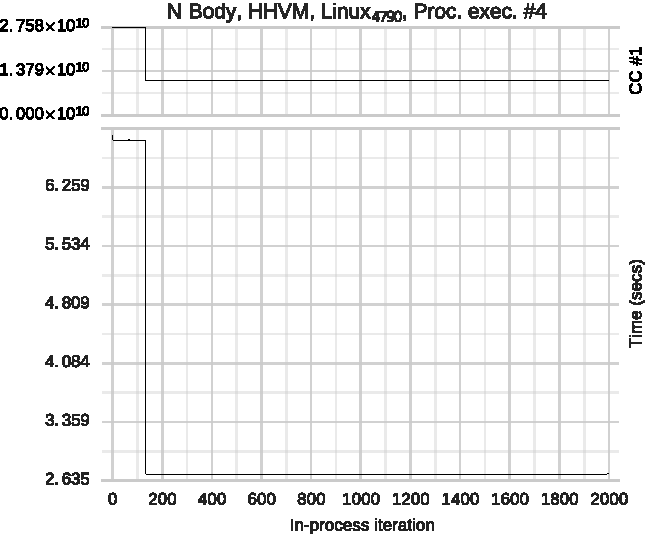
\includegraphics[width=.49\textwidth]{examples/new_warmup_no_migrate.pdf}
\hspace{\fill}
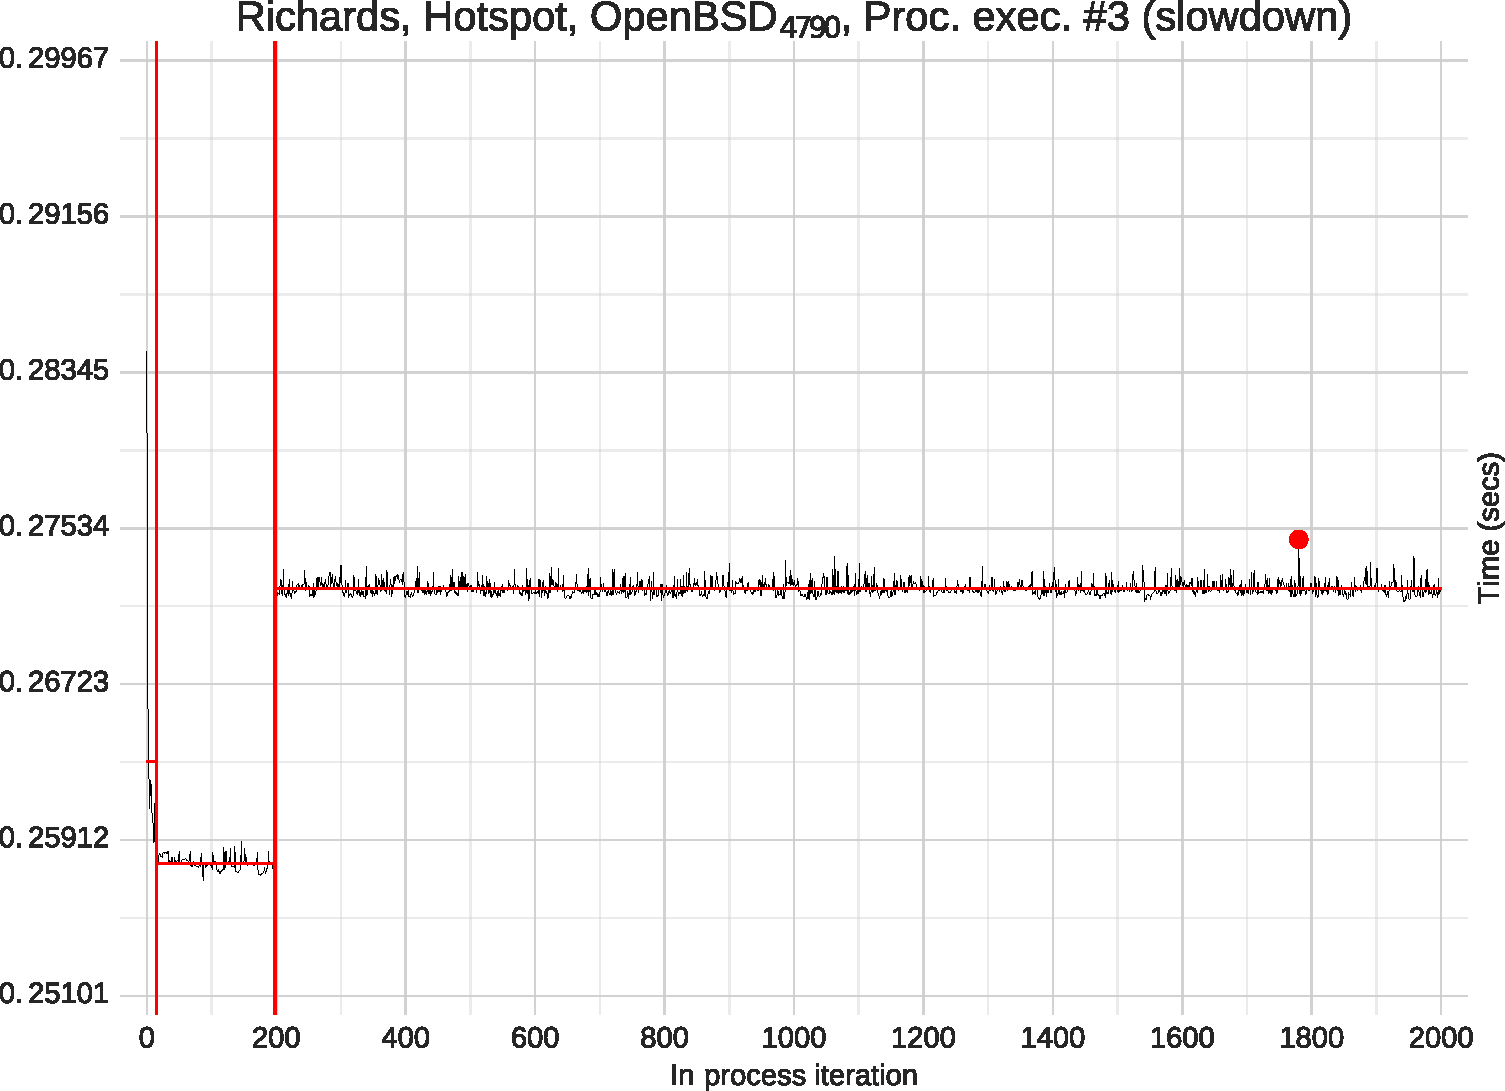
\includegraphics[width=.49\textwidth]{examples/changepoint_example.pdf}
\caption{Two example run-sequence plots from our results, augmented
with the results of changepoint analysis. The LHS plot
shows an example of `traditional' warmup (in this case \binarytrees on HotSpot);
the RHS plot shows an example of slowdown (\richards on HotSpot). The
plot titles show: the benchmark (e.g.~\binarytrees), the VM (e.g.~HotSpot),
the machine (e.g.~\bencherfive), the process execution number (e.g.~5),
and the classification (e.g.~warmup). The `main' plot at the bottom always shows
the in-process iteration number (indexed from 1) and the corresponding wall-clock
times for all \numiterations in-process iterations. Because this often obscures the finer
details, we also show two additional visualisations of the data: the top plot
shares its $x$ axis with the bottom plot, but zooms the $y$ axis in to where the bulk of the
in-process timing data is located; the smaller inset plot allows us to examine a handful
of in-process iteration timings (typically, though not always, the first $n$,
allowing us to see the `warmup curve', if it exists). Changepoints
are indicated by dashed vertical red lines and denote a `shift' in performance behaviour;
changepoint segments are indicated by dashed horizontal red lines between changepoints,
whose height shows the mean iteration time within the segment;
and red circles indicate `outliers', which the changepoint analysis discount. We use the changepoint
segments to determine if and when a steady state has been reached and,
if so, to classify the plots' warmup style (in this example, warmup and
slowdown respectively). As an additional visual aid, changepoint segments
considered equivalent in timing to the steady state segment are plotted in black;
all other segments are plotted in grey.}
\label{fig:changepoint}
\end{figure}

We use changepoint analysis~\cite{eckley11analysis} to
automatically analyse VM benchmarking data. Changepoint analysis detects
shifts in the nature of time series data (e.g.~when a benchmark switches
from `slow' to `fast' modes after JIT compilation). We then use this
information to automatically classify each process execution as either:
no steady state; flat (no detectable change in performance
over the benchmark); warmup; or slowdown (a decrease in performance over time).
Figure \ref{fig:changepoint} shows an example of how changepoint analysis
can automatically classify both `good' and `bad' warmup styles.
Although simple, these classifications allow us to tease apart
unexpected performance patterns that previous methodologies cannot.

Finally, in an attempt to see if there are easy explanations for the odd
effects we see, we take two VMs and separate out the
time taken to perform Garbage Collection (GC) and JIT compilation. These
two factors explain only some of the effects we see.


\subsection{Summary}

In summary, this paper's contributions are as follows:
\begin{enumerate}
    \item We show that, even in a highly idealised setting, widely studied benchmarks
often fail to reach a steady state of peak performance.
    \item We present the first automated approach to analysing time series
data from VM benchmarking, which can automatically determine if and when a steady
state has been reached.
    \item We present the first classification of different styles of
steady state behaviour (warmup, slowdown, flat).
    \item We show that, while some instances of `odd' behaviour are explained by
the `obvious' factors of GC and JIT compilation, many are not.
\end{enumerate}

The statistical approach we have developed is open-source, general, and can be used
to analyse any VM benchmarking data. In the Appendix, we show it applied
to the DaCapo and Octane benchmark suites,
both run in a conventional manner (Appendix~\ref{sec:existing}). We also present a curated
series of plots of interesting data (Appendix~\ref{sec:curatedplots}). A
separate document contains the complete plots of all data from all machines.

Our repeatable experiment, as well as the specific results used
in this paper, can be downloaded from:
\url{https://archive.org/download/softdev_warmup_experiment_artefacts/v0.8/}


\section{Background}
\label{sec:warmup}

When a program begins running on a JIT compiling VM, it is typically (slowly)
interpreted; once `hot' (i.e.~frequently executed) loops or methods are
identified, they are dynamically compiled into machine code; and subsequent
executions of those loops or methods use (fast) machine code rather than the
(slow) interpreter. Once machine code generation has completed, the VM is
said to have finished warming up, and the program is said to be executing
at a steady state of peak performance.\footnote{The traditional view applies equally to VMs
that perform immediate compilation instead of using an interpreter, and to
those VMs which have more than one layer of JIT compilation (later JIT
compilation is used for `very hot' portions of a program, trading slower
compilation time for better machine code generation).}
While the length of the warmup period
is dependent on the program and JIT compiler, all JIT compiling
VMs are based on this performance model~\cite{kalibera13rigorous}.

Benchmarking of JIT compiled VMs typically focusses on reporting
steady state numbers based on two assumptions: first, that warmup is both fast and
inconsequential to users; second, that the steady state is also peak performance.
The methodologies used are typically straightforward: benchmarks are run for a number
of in-process iterations within a single VM process execution.
The first $n$ in-process iterations
are then discarded, on the basis that warmup \emph{should} have completed in
that period. Often $n$ is a fixed number (typically around 5), with no guarantee
that warmup has completed by that point. More advanced methods such as
that of~\citet{georges07statistically} try to find a steady state
using simple statistical tests.

The most sophisticated VM benchmarking analysis yet developed is found
in~\cite{kalibera12quantifying,kalibera13rigorous}. After
showing that simple heuristics such as Georges et al.'s often fail to accurately
pinpoint when warmup has completed, \kalibera then present an alternative manual
process. In essence, after a specific VM / benchmark combination has been run for a small number of
process executions, a human must determine if a steady state is reached;
and, if it is, at which in-process iteration
it is reached. When a steady state does exist, a larger number of process executions are then
run; the previously determined cut-off point is applied to each process execution's
in-process iterations; and detailed statistics are produced.

The \kalibera methodology is a significant advance on previous work,
and is an important inspiration for ours. However, the reliance
on manually identifying when warmup is complete has ramifications. Most
obviously, humans are prone to error and disagreement when performing
such identifications. More significantly, the time required
to manually examine the time series data means that it is only practical to apply it to a small number
of initial process executions: the cut-off point that is determined from those
is then applied to all future process executions, even though there is no
guarantee that they all reach a steady state by that point. With
the exception of in-process iterations which show dependence in their data (e.g.~a
repeated `cyclic' pattern), which are dealt with specially,
\kalibera do not otherwise classify
steady state performance relative to what came before it, making
it hard to understand if the steady state represents peak performance
or not. These three points mean that,
despite \kalibera's advances,
``determining when a system has warmed up, or even providing a
rigorous definition of the term, is an open research problem''~\cite{seaton15phd}.


\section{Methodology}
\label{sec:methodology}

To test Hypothesis \hypone, we designed an experiment which uses a suite of
microbenchmarks: each is run with \numiterations in-process iterations and repeated
using \numpexecs process executions. We have carefully designed our
experiment to be repeatable and to control as many potentially confounding variables as
is practical. In this section we detail: the benchmarks we used and the modifications we
applied; the VMs we benchmarked; the machines we used for benchmarking; and the
\krun system we developed to run benchmarks.

First time readers of this paper may find it easiest to jump straight to
Section~\ref{sec:stats}, coming back to the complete (lengthy!) methodology
on a second read.


\subsection{The Microbenchmarks}
\label{sec:microbenchmarks}

The microbenchmarks we use are as follows: \binarytrees, \spectralnorm, \nbody,
\fasta, and \fannkuch from the Computer Language Benchmarks Game (CLBG)~\cite{clbg}; and
\richards. Readers can be forgiven for initial scepticism about this set of microbenchmarks.
They are small and widely
used by VM authors as optimisation targets. In general they are more effectively
optimised by VMs than average programs; when used as a proxy for other types
of programs (e.g.~large programs), they tend to overstate the effectiveness of
VM optimisations (see e.g.~\cite{ratanaworabhan09jsmeter}). In our context, this weakness is in fact a strength:
small, deterministic, and widely examined programs are our most
reliable means of testing Hypothesis \hypone. Put another way, if we were to run arbitrary programs
and find unusual warmup behaviour, a VM author might reasonably counter that
``you have found the one program that exhibits unusual warmup behaviour''.

For each benchmark, we provide versions in C, Java, JavaScript, Python, Lua, PHP,
and Ruby. Since most of these
benchmarks have multiple implementations in any given language, we picked
the versions used in~\cite{bolz14impact}, which represented the fastest
performers at the point of that publication. We lightly modified
the benchmarks to integrate with our benchmark runner (see Section~\ref{krun})
but did not e.g.~force garbage collection.


\subsubsection{Ensuring Determinism}

User programs that are deliberately non-deterministic are unlikely to
warm-up in the traditional fashion.
We therefore wish to guarantee that our benchmarks are,
to the extent controllable by the user, deterministic, taking
the same path through the Control Flow Graph (CFG)
on all process executions and in-process iterations. We make no attempt to
control non-determinism within the VM, which is part of what we need to test for
Hypothesis \hypone.

To check whether the benchmarks were deterministic at the user-level, we created
versions with \texttt{print} statements at all possible points of CFG
divergence (e.g.~inside conditional branches).
These versions are available in our experimental suite. We first ran the modified
benchmarks with 2 process executions and 20 in-process iterations,
and compared the outputs of the two processes. This was enough to show that the
\fasta benchmark was non-deterministic
in all language variants, due to its random number generator not being reseeded. We
fixed this by moving the random seed initialisation to the start
of the in-process iteration main loop.

In order to understand the effects of compilation non-determinism,
we then compiled the VMs and ran our modified benchmarks on two different machines.
We then observed occasional non-determinism in Java benchmarks.
This was due to the extra class we had added to each benchmark
to interface with the benchmark runner: sometimes, the
main benchmark class was lazily loaded after benchmark timing had started in a
way that we could observe. We
solved this by adding an empty static method to each benchmark, which our
extra classes then call via a static initialiser, guaranteeing that
the main benchmark class is eagerly loaded. Note that we do not attempt to eagerly
load other classes: lazy loading is an inherent part of the JVM specification,
and thus something that should be part of our measurements.


\subsection{Measuring Computation Rather than File Performance}

By their very nature, microbenchmarks tend to perform computations which
can be easily optimised away. While this speaks well of
optimising compilers, benchmarks whose computations
are entirely removed are rarely useful~\cite{seaton15phd}. To prevent optimisers
removing such code, many benchmarks write intermediate and final results
to \texttt{stdout}. However, this then means that one starts including
the performance of file routines in libraries and the kernel in measurements,
which can become a significant part of the eventual measure.

To avoid this, we modified the benchmarks to calculate a checksum
during each in-process iteration. At the end of each in-process iteration
the checksum is compared to an expected value; if the comparison fails then
the incorrect checksum is written to \texttt{stdout}. This idiom
lowers the chances that an optimiser can remove the main benchmark
code, even though no output is produced. We also use this mechanism to give some assurance
that the different language implementations of a benchmark are performing
roughly the same work, as the expected checksum value is the same for all
implementations of the benchmark.


\subsection{VMs under Investigation}
\label{sec:vms}

We ran the benchmarks on the following language implementations: GCC \gccversion;
Graal \graalversion (an alternative JIT compiler for HotSpot); HHVM \hhvmversion (a JIT
compiling VM for PHP); JRuby+Truffle \trufflerubyversion{} (a JIT compiling VM
for Ruby using Graal/Truffle);
HotSpot \hotspotversion (the most widely used Java
VM); LuaJIT \luajitversion (a tracing JIT compiling VM for Lua); PyPy \pypyversion (a
meta-tracing JIT compiling VM for Python 2.7); and V8 \veightversion (a JIT
compiling VM for JavaScript). A repeatable build script downloads, patches,
and builds fixed versions of each VM. All VMs were compiled with GCC/G++ \gccversion
(and GCC/G++ bootstraps itself, so that the version we use compiled itself)
to remove the possibility of variance through the use of different compilers.

\label{openbsd porting} We skipped: Graal, HHVM, and JRuby+Truffle on OpenBSD, as
these VMs have not yet been ported to this platform; \fasta on JRuby+Truffle as
it crashes; and \richards on HHVM since it takes as long as every other benchmark
on every other VM put together.


\subsection{Benchmarking Hardware}

With regards to hardware and operating systems, we made the
following hypothesis:
\begin{description}
  \item[\hyptwo] Moderately different hardware and operating systems have little effect on warmup.
\end{description}
We deliberately use the word `moderately', since significant changes of hardware
(e.g.~x86 vs.~ARM) or operating system (e.g.~Linux vs.~Windows) imply that
significantly different parts of the VMs will be used (see Section~\ref{sec:threats}).

In order to test Hypothesis \hyptwo, we used three benchmarking machines: \emph{\bencherseven}, a Xeon E3-1240 v5 3.5GHz,
24GB of RAM, running Debian 8; \emph{\bencherfive}, a quad-core i7-4790
3.6GHz, 32GB of RAM, running Debian 8; and \emph{\benchersix}, a quad-core i7-4790
3.6GHz, 32GB of RAM, running OpenBSD 6.0. \bencherseven and \bencherfive
have the same OS (with the same packages and updates etc.) but different hardware; \bencherfive
and \benchersix have the same hardware (to the extent we can determine)
but different operating systems.

We disabled turbo boost and hyper-threading in the BIOS. Turbo boost
allows CPUs to temporarily run in an higher-performance
mode; if the CPU deems it ineffective, or if its safe limits (e.g.~temperature) are exceeded,
turbo boost is reduced~\cite{charles09turboboost}. Turbo boost
can thus substantially change one's
perception of performance. Hyper-threading gives the illusion that a single
physical core is two logical cores. Programs and threads that would
otherwise run on separate physical cores are thus inter-leaved on
a single core, leading to less predictable performance.


\subsection{\krun}
\label{krun}

Many confounding variables manifest shortly before, or during the running of,
benchmarks~\cite{kalibera05precision}. In order to control as many of these as possible, we wrote
\krun\footnote{The `K' in Krun is a respectful tip of the hat to \kalibera.}.
\krun is a `supervisor'
which, given a configuration file specifying VMs, benchmarks, etc. configures
a Linux or OpenBSD system, runs benchmarks, and collects the results. Individual VMs and benchmarks
are then wrapped, or altered, to report data back to \krun in an appropriate format.

In the remainder of this subsection, we describe \krun. Since most of \krun's
controls work identically on Linux and OpenBSD, we start with those,
before detailing the differences imposed by the two operating systems. We then
describe how \krun collects data from benchmarks.
Note that, although \krun has various `developer' flags to aid development
and debugging benchmarking suites, we describe only \krun's full `production' mode.


\subsubsection{Platform Independent Controls}

A typical problem with benchmarking is that earlier process executions can
affect later ones (e.g.~a benchmark which forces memory to swap will make
later benchmarks seem to run slower). Therefore, before each process execution
(including before the first), \krun reboots the system, ensuring that each
process execution runs with the machine in a state that
is uninfluenced by previous process executions. After each reboot, \krun is
executed by the init subsystem; \krun then pauses for 3
minutes to allow the system to fully initialise; calls \texttt{sync} (to
flush any remaining files to disk) followed by a 30 second wait; before finally running the
next process execution.

The obvious way for \krun to determine which benchmark to run next is to examine
its results file. However, this is a large file which grows over time, and
reading it in could affect benchmarks (e.g.~due to significant memory
fragmentation). When invoked for the first time, \krun
creates a simple schedule file. After each reboot this is scanned
line-by-line for the next benchmark to run; the benchmark is run; and the schedule
updated, without changing its size. Once the process execution is
complete, \krun can safely load the results file in and append the results data,
knowing that the reboot that will occur shortly after will put the machine into
a (largely) known state.

Modern systems have various temperature-based limiters built in:
CPUs, for example, lower their frequency if they get too hot.
After its initial invocation, \krun waits for 1 minute before collecting
the values of all available temperature sensors. After each reboot's \texttt{sync}-wait, \krun waits
for the machine to return to these base temperatures ($\pm3\degree$C) before
starting the benchmark, fatally aborting if this temperature range is not
met within 1 hour. In so doing, we aim to lessen the impact of ambient temperature changes.

\krun fixes the heap and stack \texttt{ulimit} for all VM processes
(in our case, 2GiB heap and a 8MiB stack).\footnote{Note that Linux allows users
to inspect these values, but also to allocate memory that exceeds them.} Benchmarks are run
as the `\texttt{krun}' user, whose account and home directory are created
afresh before each process execution to prevent cached files affecting benchmarking.

User-configurable commands can be run before and after each process execution.
We disabled as many Unix daemons as possible (e.g.~smtpd,
crond) to lessen the effects of context switching. We also
turned off network interfaces entirely, to prevent outside sources causing
(potentially performance interfering) interrupts to be sent to the processor and kernel.

In order to identify problems with the machine itself, \krun monitors the
system \texttt{dmesg} buffer for unexpected entries (known `safe' entries
are ignored), informing the user if any arise. We implemented this after
noticing that one machine initially ear-marked for benchmarking occasionally
overheated during benchmarking, with the only clue to this being a line in \texttt{dmesg}.
We did not use this machine for our final benchmarking.

A process's environment size can cause measurement
bias~\cite{mytkowicz09surprising}. The diversity of VMs and platforms
in our setup makes it impossible to set a unified environment size across all VMs and
benchmarks. However, the \texttt{krun} user does not
vary its environment (we recorded the environment seen by each process
execution and verified their size), and we designed the experiment such that,
for each machine, each \vmbpair has a consistent environment size.


\subsubsection{Linux-specific Controls}

On Linux, \krun controls several additional factors, sometimes by checking that
the user has correctly set controls which can only be set manually.

\krun uses \texttt{cpufreq-set} to set the CPU governor to \texttt{performance} mode
(i.e.~the highest non-overclocked frequency possible).
To prevent the kernel overriding this setting, \krun verifies that the user has disabled
Intel P-state support in the kernel by passing
\texttt{intel\_pstate=disable} as a kernel argument.

As standard, Linux interrupts (`ticks') each core
\texttt{CONFIG\-\_HZ} times per second (usually 250) to
decide whether to perform a context switch. To avoid these repeated
interruptions, \krun checks that it is running on a `tickless'
kernel~\cite{tickless}, which requires recompiling the kernel with the
\texttt{CONFIG\_NO\_HZ\_FULL\_ALL} option set. Whilst the boot core still
`ticks', other cores only `tick' if more than one runnable process is scheduled.

Similarly, Linux's \texttt{perf} profiler may interrupt cores up to 100,000 times a
second. We became aware of \texttt{perf} when \krun's \texttt{dmesg} checks
notified us that the kernel had decreased the sample-rate by
50\% due to excessive overhead. While frequent sampling will clearly have some performance
impact, adaptive sampling is even more troubling: a change of sample
rate during a process execution could notably change performance.
Although \texttt{perf} cannot be completely disabled, \krun sets it to sample at most
once per second, minimising interruptions.


\subsubsection{OpenBSD-specific Controls}

Relative to Linux, OpenBSD exposes fewer controls to user. Nevertheless,
there are two OpenBSD specific features in \krun.
First, \krun sets CPU performance to maximum by invoking \texttt{apm -H} prior
to running benchmarks (equivalent to Linux's \texttt{performance} mode).
Second, \krun minimises the non-determinism in OpenBSD's malloc implementation,
for example not requiring \texttt{realloc} to always reallocate memory to
an entirely new location. The \texttt{malloc.conf} flags we use are \texttt{cfgrux}.


\subsubsection{The Iteration Runners}

To report timing data to \krun, we created an
\emph{iteration runner} for each language under investigation.
These take the name of a specific benchmark and
the desired number of in-process iterations, run the benchmark appropriately,
and once it has completed, print the times to \texttt{stdout} for \krun to
capture. For each in-process iteration we
measure (on Linux and OpenBSD) the wall-clock time taken, and (Linux only) core
cycle, APERF, and MPERF counters.

We use a monotonic wall-clock timer with sub-millisecond accuracy
(\texttt{CLOCK\_MONOTONIC\_RAW} on Linux, and \texttt{CLOCK\-\_MONOTONIC} on
OpenBSD). Although wall-clock time is the only measure which really matters to
users, it gives no insight into multi-threaded computations: on Linux we also record
core-cycle counts using the \texttt{CPU\-\_CLK\-\_UNHALTED\-.CORE} counter to see
what work each core is actually doing. In contrast, we use the ratio of APERF/MPERF deltas
solely as a safety check that our wall-clock times are valid.
The \texttt{IA32\_APERF} counter increments at a rate proportional to the
processor's current frequency; the \texttt{IA32\_MPERF} counter increments at a fixed
rate normalised to the CPU's base frequency. With an APERF/MPERF ratio of
precisely 1, the processor is running at full speed; below 1 it is in
a power-saving mode; and above 1, turbo boost is being used.

A deliberate design goal of the in-process iteration runners is to minimise
timing noise and distortion from measurements. Since system calls can have a
significant overhead (on Linux, calling functions such as \texttt{write} can
evict as much as two thirds of an x86's L1 cache~\cite{soares10flexsc}), we
avoid making any system calls other than those required to take measurements. We
avoid in-benchmark I/O and memory allocation by storing measurements in a
pre-allocated buffer and only writing measurements to \texttt{stdout} after all
in-process iterations have completed (see Listing~\ref{lst:pyiter} for an
example). However, the situation on Linux is complicated by our need to read
core-cycle and APERF/MPERF counts from Model Specific Register (MSR) file device
nodes,\footnote{We forked, and slightly modified, Linux's \texttt{msr} device
driver to allow us to easily access the MSRs as a non-root user.} which are relatively
slow (see Section~\ref{aperf/mperf error}). Since wall-clock time
is the most important measure, we ensure that it is the innermost measure taken
(i.e.~to the extent we control, it does not include the time taken to read
core-cycle or APERF/MPERF counts) as shown in Listing~\ref{lst:krun-measure}.

\begin{table}[t]
\centering
\begin{minipage}[t]{0.57\textwidth}
\begin{lstlisting}[xleftmargin=0cm]
void krun_measure(int mdata_idx) {
  struct krun_data *data = &(krun_mdata[mdata_idx]);
  if (mdata_idx == 0) { // start benchmark readings
    for (int core = 0; core < num_cores; core++) {
      data->aperf[core] = read_aperf(core);
      data->mperf[core] = read_mperf(core);
      data->core_cycles[core] = read_core_cycles(core);
    }
    data->wallclock = krun_clock_gettime_monotonic();
  } else {              // end benchmark readings
    data->wallclock = krun_clock_gettime_monotonic();
    for (int core = 0; core < num_cores; core++) {
      data->core_cycles[core] = read_core_cycles(core);
      data->aperf[core] = read_aperf(core);
      data->mperf[core] = read_mperf(core);
    }
  }
}
\end{lstlisting}
\end{minipage}%
\hfill
\begin{minipage}[t]{0.39\textwidth}
\begin{lstlisting}[xleftmargin=0cm]
wallclock_times = [0] * iters
for i in xrange(iters):
  # Start timed section
  krun_measure(0)
  # Call the benchmark
  bench_func(param)
  # End timed section
  krun_measure(1)
  wallclock_times[i] = \
    krun_get_wallclock(1) - \
    krun_get_wallclock(0)
js = { "wallclock_times": \
        wallclock_times }
sys.stdout.write(\
  "%s\n" % json.dumps(js))
\end{lstlisting}
\end{minipage}%
\\
\begin{minipage}[t]{0.57\textwidth}
\captionof{lstlisting}{\texttt{krun\_measure}: Measuring before (the \texttt{if} true branch) and
after (the false branch) a benchmark. Since
wall-clock time is the most important measure, it is innermost; since
the APERF/MPERF counters are a sanity check, they are outermost. Note that
the APERF/MPERF counters must be read in the same order before
and after a benchmark.}
\label{lst:krun-measure}
\end{minipage}%
\hfill
\begin{minipage}[t]{0.39\textwidth}
\captionof{lstlisting}{An elided version of the Python
in-process iteration runner (with core-cycles etc. removed).}
\label{lst:pyiter}
\end{minipage}%
\end{table}

The need to carefully sequence the measurements, and the fact that not all of
the VMs in our experiment give us access to the appropriate monotonic timer,
meant that we had to implement a small C library (\texttt{libkruntime.so}) to do so
(see Listing~\ref{lst:krun-measure} for an example). When possible
(all VMs apart from JRuby+Truffle, HHVM, and V8), we used a language's FFI to dynamically load this library;
in the remaining cases, we linked the library directly against the VM, which
then required us to add user-language visible functions to access them.
Core-cycle, APERF, and MPERF counts are 64-bit unsigned integers; since
JavaScript and current versions of LuaJIT do not support
integers, and since PHP's maximum integer size varies across OS and PHP versions, we
convert the 64-bit unsigned measurements to
double-precision floating point values in those VMs, throwing an error if this leads to a
loss of precision.


\section{Classifying Warmup}
\label{sec:stats}

The main data created by our experiment is the time taken by each in-process
iteration to run. Formally, this is time series data of length \numiterations. In
this Section we explain how we use statistical changepoint analysis to enable us to
understand this time series data and classify the results we see, giving the
first automated method for identifying warmup.


\subsection{Outliers}

As is common with analyses of time series data, we first identify
\emph{outliers} (in-process iterations with much larger/smaller times than their near
neighbours), which in our context are likely to be the result of JIT compilation,
GC, or of other processes interrupting benchmarks. Outliers can then be ignored
when looking for meaningful performance shifts during changepoint analysis. We use the method described
by~\citet{tukey1977exploratory}, conservatively defining an outlier as one that, within a
sliding window of 200 in-process iterations, lies outside the median $\pm
3\times(90\%\textrm{ile} - 10\%\textrm{ile})$. In order that we avoid classifying
slow warmup iterations at the start of an execution as outliers (when they are
in fact likely to be important warmup data), we ignore the first 200 in-process
iterations. Of the \num{\totaliterations}\xspace in-process
iterations, \totaloutlierspercentage\% are classified as outliers, with the most for
\FPeval{\result}{round(2000.0 / \maximumoutliers, 1)}%
any single process execution being \result\% of in-process iterations.


\subsection{Changepoint Analysis}

Intuitively, in order to uncover if/when warmup has completed, we need to
determine when in-process iteration timings have `shifted' in nature (i.e.~become
faster or slower). For example, for traditional warmup, we would expect to see a
number of in-process iterations taking time $t$ to be followed by a number at
time $t'$ (where $t' < t$). Automating the detection of such `shifts' is
tricky: simple heuristics suffer from both false positives and negatives~\cite{kalibera13rigorous}; and
`I know it when I see it' manual detection is time-consuming and prone to human
error.

Instead, we use changepoint analysis (see~\citet{eckley11analysis} for an
introduction) to determine if and when warmup has occurred. Formally, a
\emph{changepoint} is a point in time where the statistical properties of prior
data are different to the statistical properties of subsequent data; the data
between two changepoints is a \emph{changepoint segment}.
Changepoint analysis is a computationally challenging problem, requiring
consideration of large numbers of possible changepoints. A completely naive
approach requires an infeasible $2^{n-1}$ calculations ($2^{1999}$ in our context).
More sophisticated changepoint analysis algorithms reduce this to $\mathcal{O}(n^3)$.
We utilise the PELT algorithm~\cite{killick12optimal} which reduces the
complexity to $\mathcal{O}(n)$ by noting that once an
`obvious' changepoint has been discovered, it is not worth including
data before that changepoint in further searches.

There are various ways of defining when a changepoint has occurred, but the best fit
for our data is to consider changes in both the mean and variance of in-process
iterations. To automate this, we use the \texttt{cpt.meanvar} function in the R
\texttt{changepoint} package~\cite{killick14changepoint}, passing $15\log{n}$ (where
$n$ is the time series length minus the number of outliers) to the
\texttt{penalty} argument, and receiving back changepoint locations along with the mean and variance
of each changepoint segment. Whilst dependence is observed in some of
our experiment's data, the large penalty we use allows us to make an assumption
of independence~\cite{antoch97effect} (see Section~\ref{sec:threats} for details).
Figure~\ref{fig:changepoint} shows an example of changepoints and
changepoint segments in our context.


\subsection{Classifications}
\label{sec:classifications}

Building atop changepoint analysis, we can then define useful classifications
for time series data from VM benchmarks.

However, we must first
acknowledge the constraints that changepoint analysis works under: it has
no way of knowing what constitutes the `noise floor' in our problem domain; nor can it
guarantee to find identical means for very similar segments separated from
one another by a segment with a clearly distinct mean or variance.
To understand how the `noise floor' affects our analysis, it
is helpful to take an extreme example. Consider a long sequence of in-process
iterations all timed at 0.1001 seconds, followed by another long sequence timed
at 0.1002 seconds. A changepoint will be detected in the transition between the
two sequences, resulting in two changepoint segments. However, we know that in practice such a small absolute timing
delta is as likely to be the result of non-determinism inherent in a real
machine or OS as it is to be due to a benchmark or VM: it would thus be
better to consider the two segments as being equivalent. Such segments
are not always contiguous. Consider a
benchmark which, after changepoint analysis, has three segments: the first with a
mean of 1.0001 seconds, the second 1.2 seconds (perhaps whilst a JIT compiler is
in action), the third 1.0002 seconds. From our perspective, the first and final
segments are best considered as being equivalent, even though they are separated by a
segment which is clearly different. We therefore need to define a suitable tolerance
for determining if two segments are equivalent. In short running benchmarks, a
small number of external events can add an absolute level of noise: in our
experience readings often vary by a
little under 0.001s. In long running benchmarks, an individual external
event may add a relatively small amount of noise, but the cumulative
effect of many external events can add up. We found that the variance was a good
heuristic for this cumulative effect (we simply interpreted it as having units
in seconds rather than seconds squared). Combining these two notions, we thus
formally define that a segment $s_i$
is equivalent to the final segment $s_f$ if $\textrm{mean}(s_i)$
is within $\textrm{mean}(s_f) \pm \textrm{max}(\textrm{variance}(s_f), 0.001\textrm{s})$.

\begin{figure}[t]
\begin{lstlisting}[label=lst:classification, xleftmargin=0cm, caption={The
classification algorithm for an individual process execution. Given an ordered
list of segments (each with "mean", "variance", and "end" attributes, the latter
being the absolute index of the last iteration in the segment)
this function returns a string classifying the run sequence's warmup style.}]
DELTA = 0.001          # Absolute time delta (in seconds) below which segments are
                       # considered equivalent.
STEADY_STATE_LEN = 500 # How many in-process iterations from the end of the time-series
                       # data will a non-equivalent segment trigger "no steady state"?

def classify(segs):
    assert(len(segs) > 0)
    last_seg = segs[len(segs) - 1]
    lower_bound = last_seg.mean - max(last_seg.variance, DELTA)
    upper_bound = last_seg.mean + max(last_seg.variance, DELTA)
    cls = "flat"
    i = len(segs) - 2
    while i > -1:
        cur_seg = segs[i]
        i -= 1
        if cur_seg.mean + cur_seg.variance >= lower_bound \
          and cur_seg.mean - cur_seg.variance <= upper_bound:
            continue
        elif cur_seg.end > len(segs) - STEADY_STATE_LEN:
            cls = "no steady state"
            break
        elif cur_seg.mean < lower_bound:
            cls = "slowdown"
            break
        assert(cur_seg.mean > upper_bound)
        cls = "warmup"
    return cls
\end{lstlisting}
\vspace{-.75cm}
\end{figure}

With that in mind, we can define a simple classification algorithm for a process
execution, based on the special nature of the final changepoint segment. Since all our benchmarks run
for \numiterations in-process iterations we (somewhat arbitrarily) define that a process
execution reaches a steady-state if all segments which cover the last 500
in-process iterations are considered equivalent to the final segment. If
not, we classify the process execution as \emph{no steady state} (\nosteadystate).
If a steady state is reached, we are then interested as to whether: all
segments are considered equivalent, leading to a classification of \emph{flat} (\flatc);
at least one segment is faster than the final segment leading to a classification
of \emph{slowdown} (\slowdown). If a steady state benchmark is not flat or a
slowdown, then by definition the final segment must be faster than
at least one preceding segment, leading to a classification of \emph{warmup} (\warmup).
Listing~\ref{lst:classification} shows an implementation of this algorithm.
We consider benchmarks whose behaviour is either flat or warmup
as `good' (flat benchmarks may be unobservably fast warmup), while
benchmarks which are either slowdown or no steady state as `bad'.

Based on this, we can then classify a \vmbpair pair as follows:
if its process executions all share the same classification (e.g.~warmup) then
we classify the pair the same way (in this example, warmup); otherwise we classify the pair as
\emph{inconsistent}. There are then two sub-categories of inconsistent
benchmarks: `good' inconsistency (\goodinconsistent) is where all a \vmbpair pair's process
executions are either flat or warmup; and `bad' inconsistency (\badinconsistent) is
when one or more process executions are no steady state or slowdown. Good inconsistency
can occur because some benchmarks are on the edge of our ability to differentiate warmup
from flat behaviour, and we prefer to assume that we are at fault rather
than the VM. Bad inconsistency is always more troubling: it
means that, at least sometimes, users will experience poor performance.


\subsection{Steady State Timings}
\label{sec:timings}

For benchmarks whose process executions all reach a steady state (i.e.~are
any combination of \flatc, \warmup, or \slowdown) we report the number of
iterations (\emph{steady iter (\#)}) and the time in seconds (\emph{steady iter (s)}) to
reach the steady state, as well as the performance within the steady
state (\emph{steady perf (s)}).

\emph{Steady iter (\#)} and \emph{steady iter (s)} allow one to understand how long it takes
a benchmark to reach a steady state, and are made possible by our use of changepoint
analysis. Flat process executions by definition have a \emph{steady iter (\#)} of 1 and
a \emph{steady iter (s)} of 0; we elide these details for benchmarks
which are consistently flat. Benchmarks often end up with a variety of distributions
for both these measures (often, though not exclusively, seen on benchmarks
which contain a mix of flat and non-flat classifications) which makes reporting standard confidence intervals
misleading. We therefore use Inter-Quartile Ranges (IQRs) to give an indication of the
spread of values, reporting the median and 5\% and 95\% percentiles (using
linear interpolation when the percentile boundaries lie between two data points).
Non-overlapping IQRs imply a meaningful difference in the \emph{steady iter (\#)} or
\emph{(s)} values of a benchmark run on two VMs; however, since IQRs are often
widely spread, we are not always able to prove meaningful differences. To give a more
nuanced view than IQRs can report we also provide thumbnail histograms.

\emph{Steady perf (s)} roughly corresponds to the `normal' performance number reported by
traditional benchmarking methodologies. In our case, the steady state is composed of one or more
segments (see Section~\ref{sec:classifications}). We report means and
99\% confidence intervals
calculated via bootstrapping (with 100,000 iterations). Although we
assume that values within segments are
independent (see Section~\ref{sec:threats}), the values across different segments are clearly not
independent. When bootstrapping, we therefore sample values within, but never
across, segments (e.g.~if a
steady state has two segments $A$ and $B$, we bootstrap $A$ to produce $A'$ and
$B$ to produce $B'$; we then merge $A'$ and $B'$ to produce a new (bootstrapped)
steady state; we never sample values from $A$ into $B'$ or $B$ into $A'$).


\section{Results}
\label{sec:results}

\begin{table}[t]
\begin{center}
\begin{tabular}{lccc}
\toprule
Class.         & \bencherfive & \bencherseven & \benchersixdagger \\
\midrule
               & \multicolumn{3}{c}{\vmbpair pairs} \\
\flatc         & \bencherfivevmbenchpairsflatpercentage\% & \benchersevenvmbenchpairsflatpercentage\% & \benchersixvmbenchpairsflatpercentage\% \\
\warmup        & \bencherfivevmbenchpairswarmuppercentage\% & \benchersevenvmbenchpairswarmuppercentage\% & \benchersixvmbenchpairswarmuppercentage\% \\
\slowdown      & \bencherfivevmbenchpairsslowdownpercentage\% & \benchersevenvmbenchpairsslowdownpercentage\% & \benchersixvmbenchpairsslowdownpercentage\% \\
\nosteadystate & \bencherfivevmbenchpairsnosteadystatepercentage\% & \benchersevenvmbenchpairsnosteadystatepercentage\% & \benchersixvmbenchpairsnosteadystatepercentage\% \\
\goodinconsistent  & \bencherfivevmbenchpairsgoodinconsistentpercentage\% & \benchersevenvmbenchpairsgoodinconsistentpercentage\% & \benchersixvmbenchpairsgoodinconsistentpercentage\% \\
\badinconsistent  & \bencherfivevmbenchpairsbadinconsistentpercentage\% & \benchersevenvmbenchpairsbadinconsistentpercentage\% & \benchersixvmbenchpairsbadinconsistentpercentage\% \\
\midrule
               & \multicolumn{3}{c}{Process executions} \\
\flatc         & \bencherfiveflatpercentage\%          & \benchersevenflatpercentage\% & \benchersixflatpercentage\% \\
\warmup        & \bencherfivewarmuppercentage\%        & \benchersevenwarmuppercentage\% & \benchersixwarmuppercentage\% \\
\slowdown      & \bencherfiveslowdownpercentage\%      & \benchersevenslowdownpercentage\% & \benchersixslowdownpercentage\% \\
\nosteadystate & \bencherfivenosteadystatepercentage\% & \benchersevennosteadystatepercentage\% & \benchersixnosteadystatepercentage\% \\
\bottomrule
\end{tabular}
\end{center}
\caption{Relative proportions of classifiers across benchmarking machines.
Classifiers key: \flatc: flat, \warmup: warmup, \slowdown: slowdown,
\nosteadystate: no steady state, \goodinconsistent: good inconsistent,
\badinconsistent: bad inconsistent. $^\dagger$Note that \bencherfive and
\bencherseven run the same set of benchmarks, but \benchersix runs a subset
(see Section~\ref{openbsd porting}).}
\label{tab:summarystats}
\end{table}

% \bfiveresult, \bsixresult, \bsevenresult defined in preamble.
Our results consist of data for \num{\totalpexecs} process executions and \num{\totaliterations} in-process
iterations. Table~\ref{tab:summarystats} summarises the \vmbpair pairs
and process executions for each benchmarking machine. Taking \bencherseven
as a representative example,
\bsevenresult\% of \vmbpair pairs have consistently `good' warmup (i.e.~are flat, warmup,
or good inconsistent) and
\FPeval{\result}{round(\benchersevenflatpercentage+\benchersevenwarmuppercentage,1)}%
\result\% of all process executions have `good' warmup (for comparison, \bencherfive
is
\bfiveresult\% and
\FPeval{\result}{round(\bencherfiveflatpercentage+\bencherfivewarmuppercentage,1)}%
\result\% respectively and \benchersix is
\bsixresult\% and
\FPeval{\result}{round(\benchersixflatpercentage+\benchersixwarmuppercentage,1)}%
\result\% respectively, though the latter runs fewer benchmarks).
Fewer \vmbpair pairs than process executions have `good'
warmup because some inconsistent \vmbpair pairs have some `good' warmup
process executions as well as some `bad'. On \bencherseven
\benchersevenvmbenchpairsslowdownpercentage\% of \vmbpair pairs slowdown,
\benchersevenvmbenchpairsnosteadystatepercentage\% of \vmbpair pairs are no steady state,
but the biggest proportion by far is `bad' inconsistent at \benchersevenvmbenchpairsbadinconsistentpercentage\%
(\bencherfive has very similar proportions). This latter figure clearly shows a
widespread lack of predictability: in almost half of cases, the same benchmark
on the same VM on the same machine has more than one performance characteristic.
It is tempting to pick one of these performance characteristics -- VM
benchmarking sometimes reports the fastest process execution, for example -- but
it is important to note that \emph{all} of these performance characteristics are
valid and may be experienced by real-world users.

Table~\ref{tab:summarystats} clearly shows that the results from \bencherseven
and \bencherfive (both running Linux but on quite different hardware) are
comparable, with the relative proportions of all measures being only a few
percent different. \benchersix (running a different OS to \bencherfive, but on similar hardware)
is however fairly different, with \benchersixvmbenchpairsbadinconsistentpercentage\%
of \vmbpair pairs being `bad' inconsistent. This is partly due to the absence of
JRuby+Truffle which, on Linux, is the most consistent
(see Section~\ref{openbsd porting}). Of the benchmarks \benchersix can run, most behave
roughly similarly (as can be seen indirectly from Table~\ref{tab:summarystats}), but
there is a more even spread of process execution classifications across \vmbpair pairs.
Tables~\ref{tab:bencher5results} and~\ref{tab:bencher6results} in the Appendix
contain further details. Overall, we believe that our results are a
somewhat clear validation of Hypothesis \hyptwo.

Looking at one machine's data brings out further detail. For
example, Table~\ref{tab:mainresults} (with data from \bencherseven)
enables us to make several observations. First, of the 6 benchmarks, only \nbody and \spectralnorm
come close to `good' warmup behaviour on all VMs (though each has 1 or 2 bad
inconsistent cases). Second, \binarytrees seems generally to be bad inconsistent,
and \fasta and \richards often bad inconsistent. This raises the question as to whether some
aspect of these benchmarks makes inconsistent performance more likely,
though they share no particularly obvious characteristics.
Third, the overall spread of steady state iter (\#) values is uneven: VMs seem
to mostly either reach a steady state quickly (often in 10 or fewer in-process
iterations) or take hundreds of in-process iterations. The latter are troubling
because previous benchmarking methodologies
will not have run the benchmarks long enough to see the steady state emerge.
Fourth, it does not seem to be the case that VMs which take a long
time to reach a steady state have faster steady states: if anything,
the opposite appears to be true, suggesting that users of some code
on some VMs suffer from a `double whammy' of poor warmup and poor
steady state performance.


\begin{landscape}
\begin{table*}[p]
\vspace{-.35cm}
% If this table gets any wider, the caption falls off the edge of the page :(
\begin{adjustbox}{scale=.85}
\input{bencher7.table}
\end{adjustbox}
\caption{Results for \bencherseven. We
report the classification of each process execution and, for inconsistent benchmarks,
the constituent classifications (e.g.~\badinconsistent(22\slowdown, 8\warmup)
means 22 slowdowns and 8 warmups). If a
steady state is achieved, we report three summary statistics. \emph{Steady iter
(\#)} is the median in-process iteration number to reach the steady state,
and \emph{Steady iter (s)} is the median wall-clock time (since the beginning of
the process execution) to reach the steady state; for both measures we
report 5\% and 95\% inter-quartile ranges. \emph{Steady perf (s)} is the mean
steady state performance across all process executions (reported with 99\%
confidence intervals). Thumbnail histograms
show the spread of values; the red bars indicates the median values.}
\label{tab:mainresults}
\end{table*}
\end{landscape}


\begin{figure}[t]
\centering
\begin{minipage}[t]{0.485\textwidth}
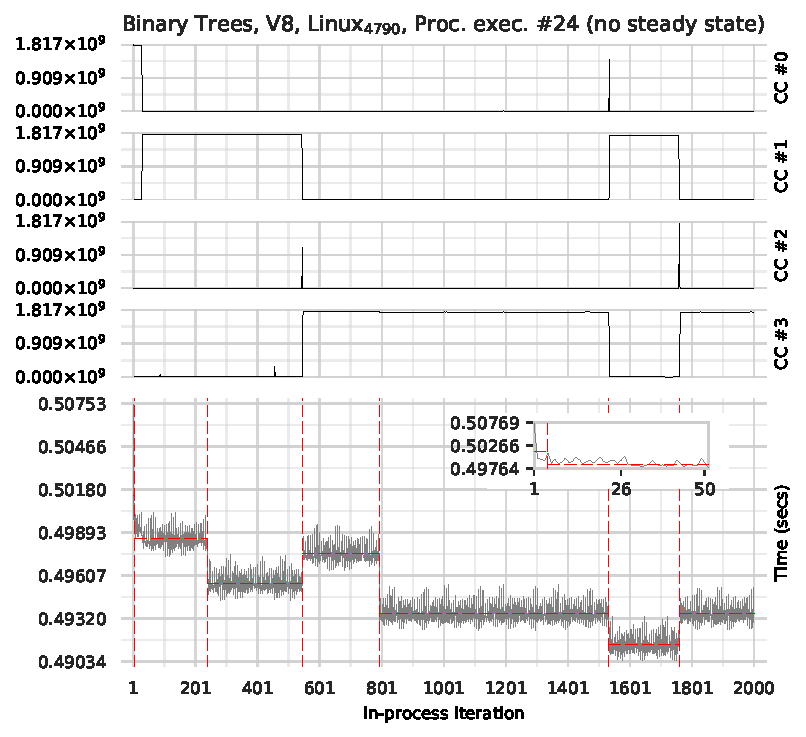
\includegraphics[width=\textwidth]{examples/new_no_steady.pdf}
\caption{An example of a run-sequence plot with core-cycle plots (one
for each of the 4 CPU cores; note that they all have the same $y$ axis scale). In this
example we can clearly see a benchmark migrating between cores. In some
cases this migration also aligns with a clear changepoint, though not
in others. The continual changepoints lead to an overall classification
of no steady state.}
\label{fig:examples:nosteadystate}
\end{minipage}%
\hfill%
\begin{minipage}[t]{0.485\textwidth}
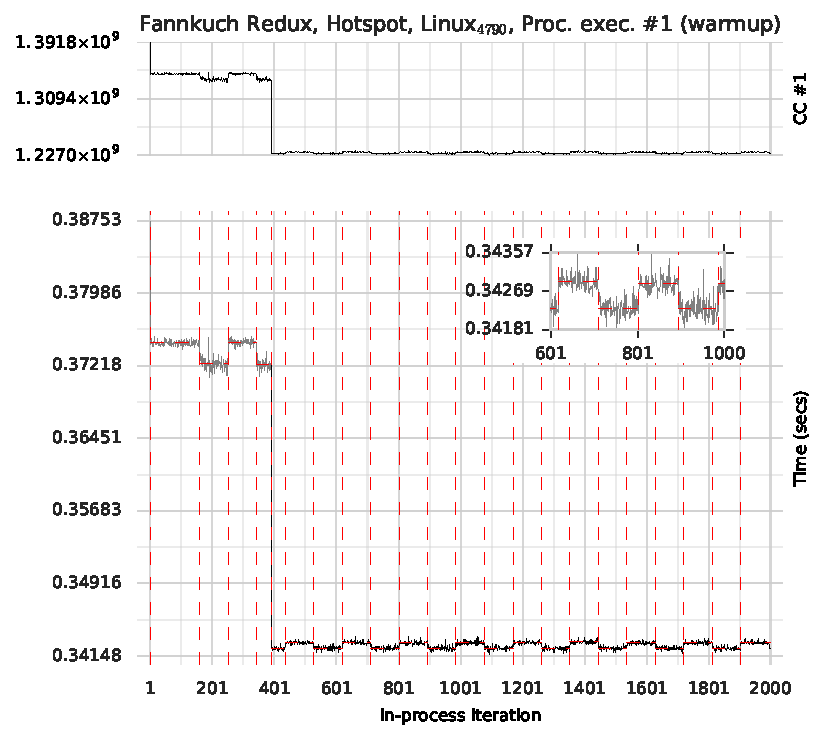
\includegraphics[width=\textwidth]{examples/new_cyclic.pdf}
\caption{Cycles in wall-clock times which are reflected by the core-cycle count
for the relevant core. Although the changepoint analysis has captured the
cycles, the change in performance is too small for the classification algorithm
to consider this example `no steady state'.}
\label{fig:examples:cycles}
\end{minipage}
\end{figure}

\begin{figure*}[t!]
\centering
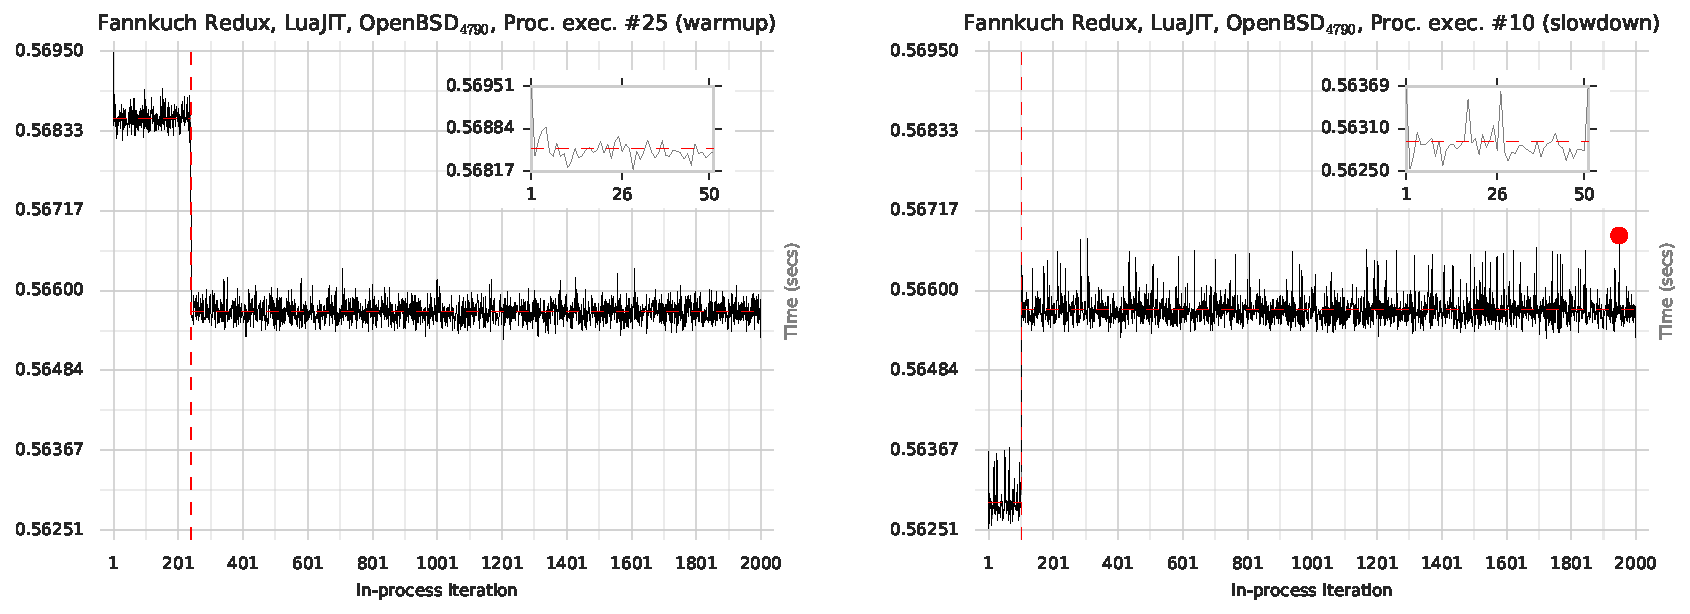
\includegraphics[width=\textwidth]{examples/new_inconsistent.pdf}
\caption{An example of bad inconsistency: the same benchmark, on
the same VM, on the same machine, with one process execution warming
up and the other slowing down.}
\label{fig:examples:inconsistent}
\vspace{-.4cm}
\end{figure*}

\begin{figure*}[t]
\centering%
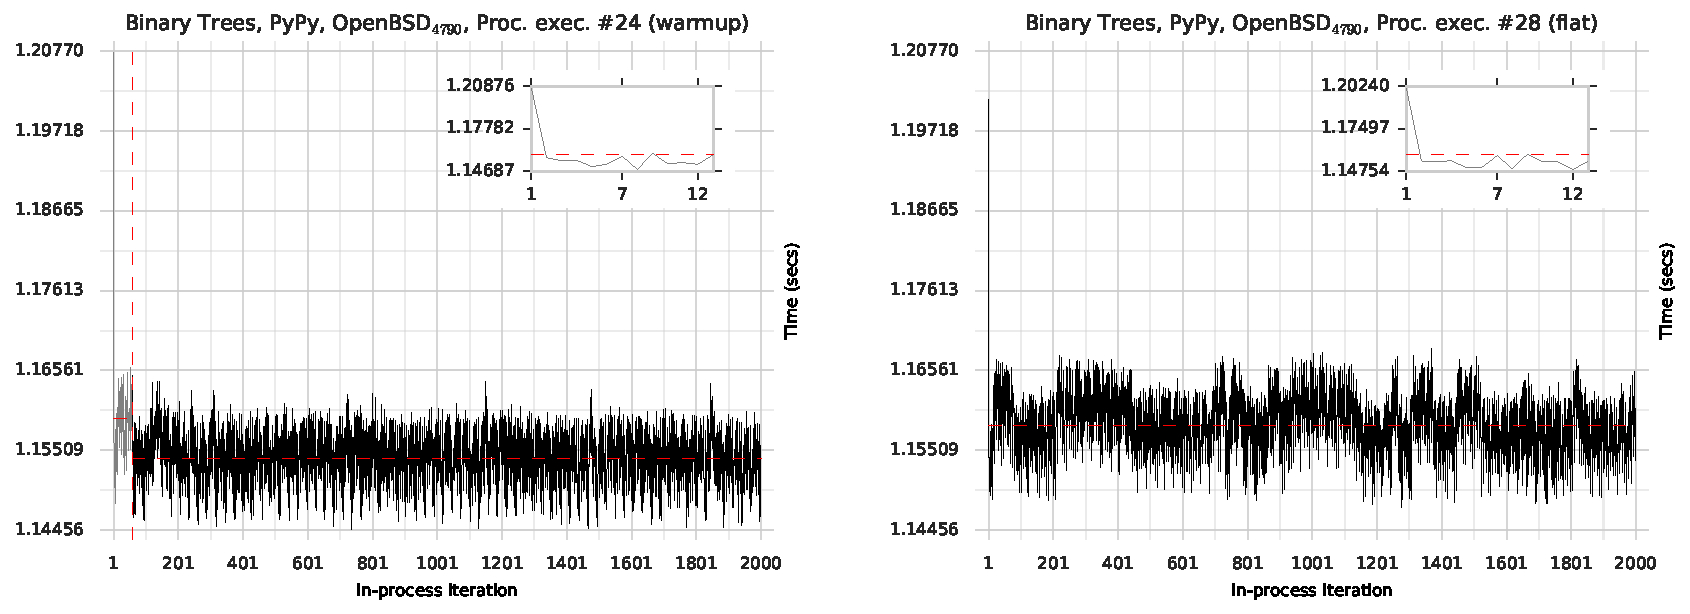
\includegraphics[width=\textwidth]{examples/warmup_flat.pdf}
\caption{An example of good inconsistency where one process execution
is classified as warmup, the other flat. Although a human might consider
both of these as warmup, there is a subtle difference in the nature of the first 20--30
in-process iterations in the LHS and RHS plots, which leads changepoint
analysis to consider the RHS plot as a single changepoint segment.}
\label{fig:examples:warmup_flat}
\vspace{-.4cm}
\end{figure*}


\begin{figure}[!tbp]
\centering
\begin{minipage}[t]{0.485\textwidth}
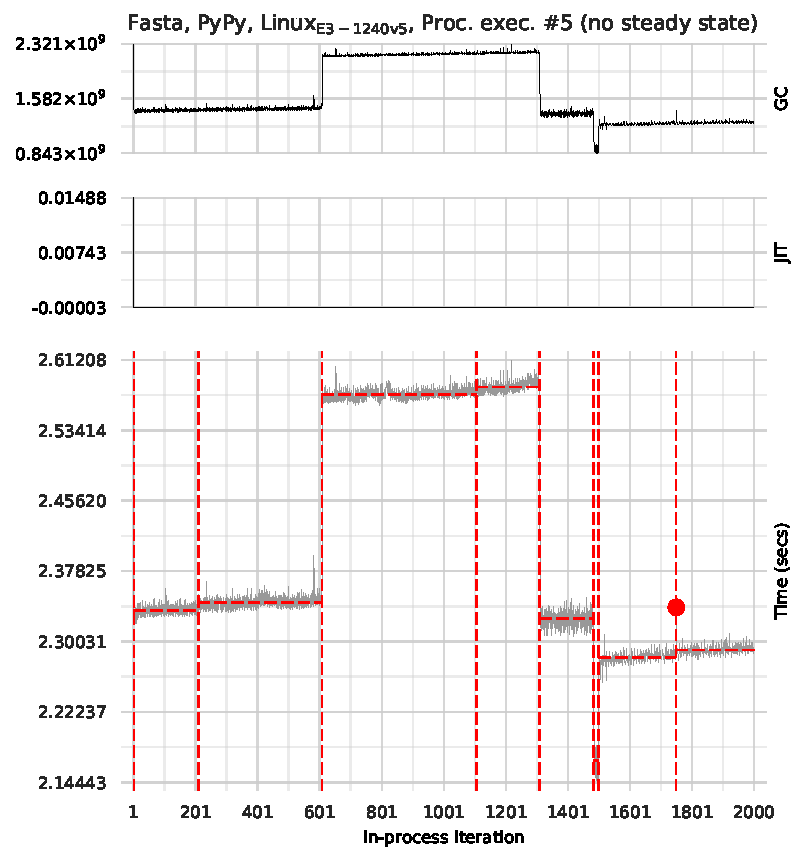
\includegraphics[width=\textwidth]{examples/new_good_comp.pdf}
\caption{A run-sequence plot (bottom) with GC (top) and JIT (middle) plots.
In this case, the benchmark's gradually increasing wall-clock time clearly
correlates with GC. This example (along with several others) appears to show a
memory leak in PyPy, which we have reported upstream.}
\label{fig:goodcomp}
\end{minipage}
\hfill
\begin{minipage}[t]{0.485\textwidth}
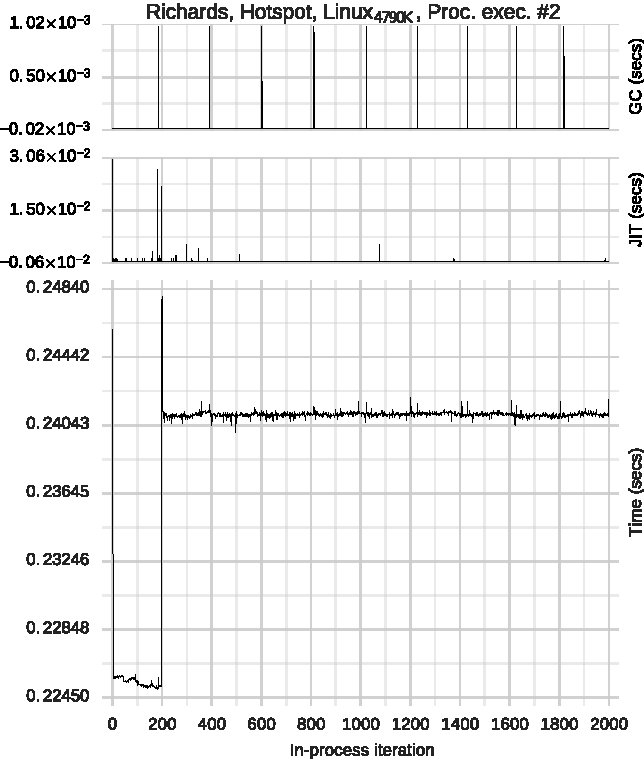
\includegraphics[width=\textwidth]{examples/new_miscomp.pdf}
\caption{Slowdown at in-process iteration \#199, which correlates
with two immediately preceding JIT compilation events
that may explain the drop in performance. Note that the
regular GC spikes have only a small effect on wall-clock time.}
\label{fig:examples:slowdown1}
\end{minipage}
\end{figure}


\subsection{Warmup Plots}

We created several different types of plot to help us understand our data in detail.
All plots have in-process iteration number on the
$x$-axis. Run-sequence plots show wall-clock times on the $y$-axis. The
plots in Figure~\ref{fig:changepoint} show run-sequence plots for warmup and
slowdown behaviours. Figure~\ref{fig:examples:inconsistent} shows an example of bad inconsistency and
Figure~\ref{fig:examples:warmup_flat} of good inconsistency. Core-cycle plots (Linux only) show the
core-cycle counts on the $y$-axes (one plot per-core). The plots in
Figures~\ref{fig:examples:nosteadystate} and \ref{fig:examples:cycles} show
examples of run-sequence plots accompanied by core-cycle plots for no steady
state and cyclic data respectively.

Core-cycle plots help us understand how VMs use, and how the OS schedules,
threads. Benchmarks running on single-threaded VMs are characterised by a high
cycle-count on one core, and very low (though never quite zero) values on all
other cores. VMs may migrate between cores during a process
execution, as can be clearly seen in Figure~\ref{fig:examples:nosteadystate}.
Although multi-threaded VMs can run JIT compilation and / or GC in parallel,
it is typically hard to visually detect such parallelism as it tends to be
accompanied by frequent migration between cores.
However, it can often be seen that several cores are active during the first few
in-process iterations whilst JIT compilation occurs.


\subsection{The Effects of Compilation and GC}
\label{sec:deepdive}

The large number of non-warmup cases in our data led us to make the following hypothesis:
\begin{description}
  \item[\hypthree] Non-warmup process executions are largely due to JIT compilation or GC events.
\end{description}
To test this hypothesis, we made use of the debug facilities of HotSpot and PyPy to
record the time spent performing JIT compilation and GC. Since
recording this additional data could potentially change the results we collect,
it is only collected when \krun is explicitly set to `instrumentation mode'.
This allows us to identify interesting correlations (though we make no claim
that they prove causation). For example,
Figure~\ref{fig:goodcomp} shows an
example where slowdown is clearly correlated to garbage collection.
Similarly, in Figure~\ref{fig:examples:slowdown1}, there is a clear correlation
between a JIT compilation and a slowdown.
However, in many cases such as Figure~\ref{fig:unexplained} neither JIT
compilation, nor garbage collection, are sufficient to explain odd
behaviours.

The relatively few results we have with GC and JIT compilation events, and the lack of a clear
message from them, means that we feel unable to validate or invalidate
Hypothesis \hypthree. Whilst some non-warmups are plausibly explained by GC or JIT compilation events, many are not, at
least on HotSpot and PyPy. When there is no clear correlation, we have very little idea of
a likely cause of the unexpected behaviour. It may be that obtaining similar data
from other VMs will clarify this issue, but not all VMs support this
feature and, in our experience, those that do support it do not always
document it accurately.

\begin{table}[t]
\begin{minipage}[t]{0.485\textwidth}%
\vspace{0pt}
\centering
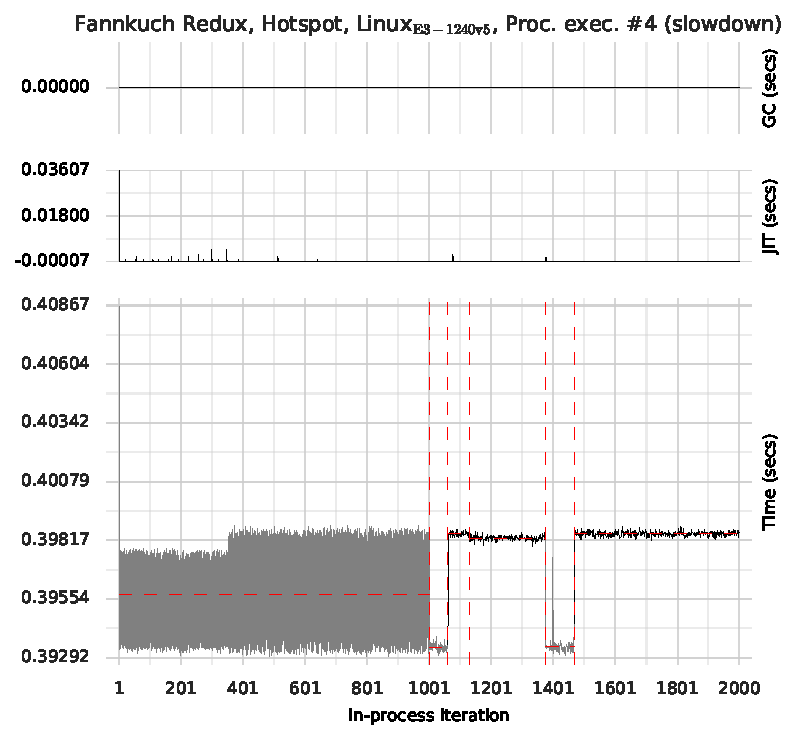
\includegraphics[width=\textwidth]{examples/unexplained_weirdness.pdf}
\end{minipage}
\hfill
\begin{minipage}[t]{0.485\textwidth}
\vspace{0pt}
\centering
\input{startup.table}
\end{minipage}
\\
\begin{minipage}[t]{0.485\textwidth}
\vspace{-\baselineskip}
\centering
\captionof{figure}{An example where performance changes do not appear to correlate with compilation or GC.}
\label{fig:unexplained}
\end{minipage}
\hfill
\begin{minipage}[t]{0.485\textwidth}
\vspace{0pt}
\centering
\captionof{table}{VM startup time (in seconds with 99\% confidence intervals).}
\label{fig:startup}
\end{minipage}
\end{table}


\section{Startup Time}
\label{sec:startup}
The data presented thus far in the paper has all been collected after the VM has
started executing the user program. The period between a VM being
invoked and it executing the first line of the user program is the VM's \emph{startup} time,
and is an important part of a VM's real-world performance.

A small modification to \krun enables us to measure startup. We prepend each VM
execution command with a small C wrapper, which prints out wall-clock time
before immediately executing the VM itself; and, for each language under
investigation, we provide a `dummy' iterations runner which simply prints out
wall-clock time. In other words, we measure the time just before the VM is loaded
and at the first point that a user-level program can execute code on the VM; the
delta between the two is the startup time. For each VM we run \numstartuppexecs process
executions (for startup, in-process iterations are irrelevant,
as the user-level program completes as soon as it has printed out wall-clock
time).

Table~\ref{fig:startup} summarises our startup results. Since
\krun reboots before each process execution, these are measures of a `cold'
start and thus partly reflect disk speed etc. (though our machines load VMs
from an SSD). As this data clearly shows, startup time varies significantly amongst VMs:
taking C on Linux as a baseline, the fastest VM (LuaJIT) is $5\times$ slower, whilst the
slowest VM (JRuby+Truffle) is around $3500\times$ slower, to startup.


\section{Threats to Validity}
\label{sec:threats}

While we have designed our experiment as carefully as possible, we do not
pretend to have controlled every possibly confounding variable. It
is inevitable that there are further confounding variables that
we are not aware of, which may have coloured our results.

We have tried to gain an understanding of the effects of different
hardware on benchmarks by using machines with the same OS but
different hardware.
More distinct hardware (e.g.~a non-x86 architecture)
is likely to uncover further hardware-related differences.
However, hardware cannot be varied in isolation from software:
the greater the differences in hardware, the more likely that JIT compilers
are to use different components (e.g.~different code generators).
Put another way, an apples-to-apples comparison across very different
hardware is often impossible, because the `same' software is itself different.

We have not systematically tested whether rebuilding VMs affects warmup, an
effect noted by \kalibera, though which seems to have little effect on
the performance of JIT compiled code~\cite{barrett15approaches}. However, since measuring warmup largely
involves measuring code that was not created by a JIT compiler, it is possible
that these effects may affect our experiment. To a limited extent, the
rebuilding of VMs that occurred on each of our benchmarking machines gives
some small evidence as to this effect, or lack thereof.

The checksums we added to benchmarks ensure that, at a user-visible level, each benchmark
performs equivalent work in each language variant. However, it is impossible to
say whether each performs equivalent work at the lowest level or not. For
example, choosing to use a different data type in a language's core library may
substantially impact performance. There is also the perennial problem as to the
degree to which an implementation of a benchmark should respect other
language's implementations or be idiomatic (the latter being likely to
run faster). From our perspective, this is somewhat less important,
since we are interested in the warmup patterns of reasonable programs,
whether they are the fastest possible or not. It is however possible that by
inserting checksums we have created unrepresentative benchmarks, though
this complaint could arguably be directed at the unmodified benchmarks too.

Although we have minimised the number of system calls that our in-process
iterations runners make, we cannot escape them entirely. For example,
on both Linux and OpenBSD \texttt{clock\_gettime} (which we use to obtain
monotonic wall-clock time) contains what is effectively a spin-lock,
meaning that there is no guarantee that it returns within a fixed bound.
%\footnote{See \texttt{binuptime} in \texttt{sys/kern/kern\_tc.c} in the
%OpenBSD source code and \texttt{getrawmonotonic} in
%\texttt{kernel/time/timekeeping.c} in the Linux source code.}
Fortunately, in practise, \texttt{clock\_gettime} returns far quicker than the granularity
of any of our benchmarks. \label{aperf/mperf error} The situation
on Linux is complicated by our reading of core-cycle, APERF, and MPERF
counters via MSR device nodes: we call \texttt{lseek} and \texttt{read}
between each in-process iteration (we keep the files open across all
in-process iterations to reduce the open/close overhead).
These calls are more involved than \texttt{clock\_gettime}:
as well as the file system overhead, reading from a MSR device
node triggers inter-processor interrupts to schedule an \texttt{RDMSR}
instruction on the desired core (causing the running core to save its registers etc.).
We are not aware of a practical way to lower these costs.

Although \krun does as much to control CPU clock speed as possible, modern CPUs
do not always respect operating system requests. On Linux, we use the
APERF/MPERF ratio to check for frequency changes. Although the hoped-for
ratio is precisely 1, there is often noticeable variation around this value due to the
cost of reading these counters. On active cores the error is small (around 1\% in our
experience), but on idle cores (which are rarely truly idle, as occasional
computation happens on them) it can be relatively high (10\% or more is
not uncommon; in artificially extreme cases, we have observed up to 200\%).
We first need to exclude idle cores from any checks. Formally
the rate at which APERF increments is undefined~\cite{intel17pstate}. In
practise, however, our machines increment APERF on a fully utilised core at the CPU base frequency
(e.g.~ \bencherfive's CPU increments APERF at $3.6$GHz).
We therefore define an idle core to be one whose APERF is 1000$\times$ less than this (per
second). We then need to determine a sensible tolerance around the ideal APERF/MPERF ratio of 1,
taking into account the error introduced by reading these counters.
For the 4790 processor, the frequency values either side of its 3.6GHz base
are 3.4GHz and 3.8GHz, which would lead to a 5\% difference in the APERF/MPERF
ratio (for the 3.5GHz E3-1240 processor, the values either side are 3.3GHz and 3.9GHz i.e.~at
least a 6\% difference in the APERF/MPERF ratio). Based on this, we define the
safe APERF / MPERF ratio to be $1\pm0.03$.\footnote{This means that small
portions of an in-process iteration could be subject to frequency changes yet still fall within
this tolerance. Given the error in reading the APERF and MPERF counters, this is an
inevitable problem; by making our tolerance relatively tight, we minimise the
chances of missing genuine issues.} We then wrote a simple tool to examine
every process execution on \bencherfive and \bencherseven, checking that every
\FPeval{\result}{round(\bencherfivetotaliterations+\bencherseventotaliterations,0)}%
active core had a safe APERF/MPERF ratio. Of the \num{\result}\xspace in-process iterations
on these two machines, 225 (0.004\%) spread over 10 process executions failed
this check, all but 2 on \bencherseven. Fortunately, outlier detection is designed
to deal with such aberrations, and 216 (98\%) of these in-process iterations are
detected as outliers. Since outliers do not affect changepoint analysis or
the statistics we produced, 8 of the 10 process executions are not affected in practise.
Since the 2 in-process iterations on \bencherfive do not have noticeably different wall-clock
times than their neighbours, and both have an APERF/MPERF ratio of 1.031
(only marginally above our safe threshold), we do not consider them problematic.
The remaining 7 in-process iterations which are not
detected as outliers are contained in 1 process execution of Graal running
\fasta: manual inspection shows that these in-process iterations are fairly
evenly spread over the (somewhat noisy) process execution and that two of them led
to a small changepoint segment that causes the process execution to be
classified as no steady state rather than warmup. As this \vmbpair pair was
\badinconsistent(29\warmup, 1\nosteadystate), it is likely that if
the processor had run at full speed, the overall benchmark
would have been classified as warmup (as indeed it was
on \bencherfive). However, overall, the similar figures
for \bencherfive and \bencherseven shown in Table~\ref{tab:summarystats} are
strong evidence of the limited effect this is likely to have had on our results.

Our experiments allow the kernel to run on the same core as benchmarking code.
We experimented extensively with CPU pinning, but eventually abandoned it. After
being confused by the behaviour of Linux's \texttt{isolcpus} mechanism (whose
semantics changes between a normal and a real-time kernel), we used CPU shielding
(\texttt{cset shield}) to pin the benchmarks to the 3 non-boot cores on our
machines. However, we then observed notably worse performance for VMs such as
HotSpot. We suspect this is because such VMs query the OS for the number of
available cores and create a matching number of compilation threads; by reducing
the number of available cores, we accidentally forced two of these threads to
compete for a single core's resources.

Address Space Layout Randomisation (ASLR) is, from a performance perspective, a
controversial feature. It clearly introduces significant non-determinism into
benchmarking, and it is thus tempting to turn it off. However, this then raises
the very real possibility that the one point in the ASLR space one is sampling
from is not indicative of the entire space. Ideally, we would use a system like
Stabilizer~\cite{curtsinger13stabilizer} to
sample across the search space evenly; unfortunately, we were not able to build
Stabilizer on a modern Linux system.\footnote{Stabilizer's authors hope to
produce a new version which is more easily ported across OS versions, though
with no definite timescale.} Since ASLR cannot be turned off on OpenBSD,
we left ASLR on Linux on, to make a comparison across the two easier.
By measuring \numpexecs process executions, we lessened, though did not
remove, the chances of all our measurements coming from a narrow part of the
overall search space.

In controlling confounding variables, our benchmarking environment inevitably
deviates from standard configurations. It is possible that in so doing we have
created a system where benchmarks warmup (or otherwise) in a way that few will ever see in
practise. However, our judgement is that this is a reasonable trade-off,
given that the alternative of a
system that is likely to introduce substantial noise into our readings.

Current changepoint analysis software available typically make an assumption of independence
within and across changepoint segments.  The \texttt{cpt.meanvar} function we use also makes this
assumption of independence, which our in-process iteration timings are clearly not.
We can safely use a changepoint approach that assumes independence by using a `larger'
penalty value~\cite{antoch97effect}. As this suggests, penalties are as much an
art as a science. A typical penalty for our setup is $4 \log n$ whereas we used $15 \log n$.
We manually inspected a large number of benchmarks and found that the
changepoints identified were rarely much worse, and in the vast majority of
cases better than, our initial manual attempts. Given the large number of
plots to analyse (\totalpexecs{} for the main part of the experiment), it is extremely unlikely that
we would have been able to do anywhere near as good a job manually as
changepoint analysis does automatically.

Although we only ever bootstrap within, and never across, segments (see
Section~\ref{sec:timings}), we are forced to assume that data within segments
are independent. Across all
three of our benchmarking machines, 11.8\% of process executions
showed some form of dependence in one or more changepoint segments.
The consequences of this are limited for two
reasons. First, over 99\% of steady state segments have a variance under 0.001s
(with the vast majority one or more orders of magnitude smaller than that),
which means that the confidence intervals we produce will be small no matter
what we do. Second, for our style of data the confidence intervals we
produce when dependence is present tend to demonstrate a small over-approximation.
To understand this, we ran a simulation study with the smallest (-0.968),
largest (0.668), and mean (-0.215) dependence we observed (where $0$ is
independence and $\pm 1$ is lag 1 correlation). The coverage
of the 99\% confidence intervals over 1,000 simulations was
100\%, 92\%, and 99.9\% respectively (where values over 99\% represent
negative correlation and values under 99\% represent positive correlation).
As a comparison, we also simulated independent data (using the
same seed as used in the dependent simulations) which had coverage of 98.3\%, showing
that even with independent data one may not always get precisely the expected coverage.
Overall, despite these limitations, we believe that our
approach produces statistics that are more representative of
a benchmark's performance than current approaches.


\section{Related work}
\label{sec:related}

There are two works we are aware of which explicitly note unusual warmup
patterns. Whilst running benchmarks on HotSpot,~\citet{gil11microbenchmark}
observed inconsistent process executions
(e.g.~recursiveErgodic), and benchmarks that we could classify as no
steady state (listBubbleSort) and slowdown (arrayBubbleSort). By running a
greater number of (somewhat larger) benchmarks on a number of VMs, and executing
them in a more tightly controlled execution environment, our results can be seen
as significantly strengthening Gil et al.'s observations. Our work also adds an
automated approach to identifying when warmup has occurred and classifying
run-sequence plots.

\cite{kalibera13rigorous} note the existence of what we have called cyclic behaviour, which
causes them to classify a benchmark as not reaching an independent state and
thus being unsuitable for bootstrapping as-is. In such instances, they require
the user to manually pick one part of the cycle (i.e.~always pick iteration $n$
after the steady state of each process execution) for bootstrapping, which leads
to a clear potential for bias (for one benchmark, one could pick the slow part
of the cycle, for another the fast part). As our approach automatically
identifies changepoint segments, we take a very different approach. Changepoint
analysis naturally identifies `large' cycles (i.e.~where the cycles are fairly
lengthy and/or with substantial differences between the means of the top and
bottom of the cycle) as different segments with non-equivalent means, which then
leads to a classification of no steady state. `Small' cycles either lead to
different segments with equivalent means or, more often, to a single segment.

Probably the most widely used method for detecting a steady state is that of
\citet{georges07statistically} which looks for in-process iterations where the
coefficient of variance (standard deviation divided by the mean of the relevant measurements)
falls below a threshold. Using a threshold of 0.01 -- the more
conservative of the two values suggested by Georges et al. -- we applied their
heuristic to our data. In virtually all of the cases where we found a steady
state, Georges et al.'s heuristic also finds a steady state (though not
necessarily at the same point). However, it also
finds steady states for \georgesnosteadystatepercent\% of the process executions we classify as no
steady state, including Figure~\ref{fig:examples:nosteadystate}. This confirms
the findings from \cite{kalibera13rigorous} that simple heuristics can often
give misleading statistics for VM benchmarking.


\section{Suggestions for the Community}
\label{suggestions}

We do not claim that this paper represents the end of the road in terms of VM
benchmarking methodologies: we hope and expect that this work will be superseded
by better approaches in the future. However, imperfect though it is, this paper
does clearly show problems with previous approaches to VM
benchmarking, including those this paper's authors have been involved with in the past. In this
section we make some tentative suggestions to the VM developer and user
communities based on our experience.

First, our results undermine the previous VM benchmarking orthodoxy of benchmarks
quickly and consistently reaching a steady state after a fixed number of iterations. It is clear
that many benchmarks take considerable time to reach a
steady state; that different process executions of the same benchmark reach a
steady state at different points; and that some process executions do not ever
reach a steady state. Even if one were to pick a very high number of initial in-process
iterations to discard, there is no guarantee that the remainder
would represent the steady state. Similarly, our results also show that one cannot assume
that one process execution of a \vmbpair pair is representative of others: each
process execution must be analysed individually to determine if, and when, a steady state is
reached. We believe that, in all practical cases, this means that one must use
an automated approach to analysing each process execution individually.
The open-source changepoint analysis approach presented in this paper is one such option.

Second, we believe that the traditional practise of presenting only steady state
numbers is hard to defend in the face of wildly varying warmup times. There
are several benchmarks where different VMs have steady state
performance within 2x of each other, but whose warmup differs by 100-1000x.
While such differences may be of little importance to some users,
they are important to many others. We thus hope that future VM experiments will
report: a benchmark's classification (warmup, flat, slowdown, no steady state);
and, if it reaches a steady state, when the steady state was reached (using
one or both of steady state iter (\#) or (s)) and the performance of the
steady state (steady perf (s)).

Third, it is important to make benchmarks run long enough that any measurements
taken are substantially above the noise floor. It is not uncommon to see
published benchmarks that run for 0.001s or smaller: external events such as a context switch
can have a significant (relative) effect on such small measurements,
giving one a false impression of performance. Because of this,
in our experiment changepoint segments with means less than 0.001s
apart are considered equivalent. However, running in-process iterations for long periods
of time is also somewhat undesirable. When possible, we suggest that
the fastest in-process iterations should run for around 0.5s. However, this can
sometimes be impractical: when benchmarking a set of VMs, the slowest VM may be
be an order of magnitude slower than another; even within a single VM,
in-process iterations before warmup can be one or two orders of magnitude slower
than after warmup. In such cases we suggest the minimum acceptable time for an
in-process iteration is 0.1s,

Fourth, we suspect that some of the odd results we have seen result from
over-training VM heuristics on small sets of benchmarks. The machine-learning
community's approach to this problem may apply equally well to VMs: this would involve
using a training set of benchmarks to devise heuristics, and then benchmarking
the resulting system(s) on a separate validation set of benchmarks.

Fifth, we suspect that a reliance on small suites of benchmarks means that
only small parts of VMs are being benchmarked effectively. We are increasingly
of the opinion that benchmarking quality and quantity are tightly related, and
that VMs need to be run on many more benchmarks than is typically the case.
However, collecting benchmarks is surprisingly difficult as there are few
guidelines as to what makes a good or bad benchmark, and the more constraints
one places on `acceptable' benchmarks, the harder the process becomes.
For example, in this paper we ensured that our benchmarks were deterministic. In
modern languages, where semi-random hashing of data-structures is common, many
moderately sized candidate benchmarks will be non-deterministic. As benchmark
suites grow in size, such trade-offs are likely to become more frequent: one
pragmatic solution may simply be to note which benchmarks have such properties
and to allow readers to take that into account when evaluating performance.


\subsection{How Long Should Experiments Be Run For?}
\label{how long}

Of all the techniques we have used in this paper, the most simple was the most
important: we simply ran benchmarks for much longer than suggested by previous methodologies.
Traditional VM experiments often run for 5 or 10 in-process iterations. Our data
clearly show that, when a statistically robust analysis is desired, such short
runs are insufficient. However, none of us wants to run benchmarks for any longer
than necessary. Assuming that we ran
experiments for `long enough', a reasonable question is whether we needed to run
as many process executions and as many in-process iterations as we did.

In this subsection we subset data from \bencherseven to see if using fewer
process executions or in-process iterations give similar results to using the full
data. We have chosen to define `similar' as `what proportion of the subsetted
gives the same results as Table~\ref{tab:mainresults}'\edd{`subsetted' is jarring in the previous sentence}. We report: individual
comparisons of \vmbpair pair's classifications, steady iter (\#)\footnote{Note
that since steady iter (\#) and steady iter (s) are the same measure, but with
different units, we only need to compare one of them. We arbitrarily
select steady iter (\#).}, and steady perf (s); and an `overall' comparison which
is true \edd{The `truth' of these metrics is confused a bit. Earlier you have
said these readings are proportions, not booleans. I though I knew what you
meant, but having read the next para, I don't think I do :(}
if and only if the three individual comparisons are true.

In most cases the comparisons involved are obvious. If, for example, the
original \vmbpair has 30 warmup process executions, and the subsetted \vmbpair pair
has 30 warmup process executions then the classifications comparison is
true\edd{now i'm confused, so true is 100\%?},
and the steady iter (\#) and steady perf (s) comparisons depend on comparing the
values from each set (taking into account confidence intervals). If the original
\vmbpair pair has 30 warmup process executions, and the subsetted \vmbpair pair has 30
slowdown process executions then the classifications comparison is false\edd{0\%?}, but
the steady iter (\#) and steady perf (s) comparisons comparisons are made as
before. The main complication comes from no steady state executions. If the
original and subsetted \vmbpair pair are consistently no steady state, then the
classifications comparison is true, but we do not count the steady iter (\#) and
steady perf (s) as either true or false (since no comparison can be made). If
one \vmbpair pair has a no steady state process executions but the other does
not, we define the classifications, steady iter (\#), and steady perf (s)
comparisons to be false.

\edd{I find the notions of true/false confusing. Since we don't use this
terminology after this point, should we try to avoid it entirely?}

\subsubsection{In-process iterations}

\begin{figure}[!tbp]
\centering
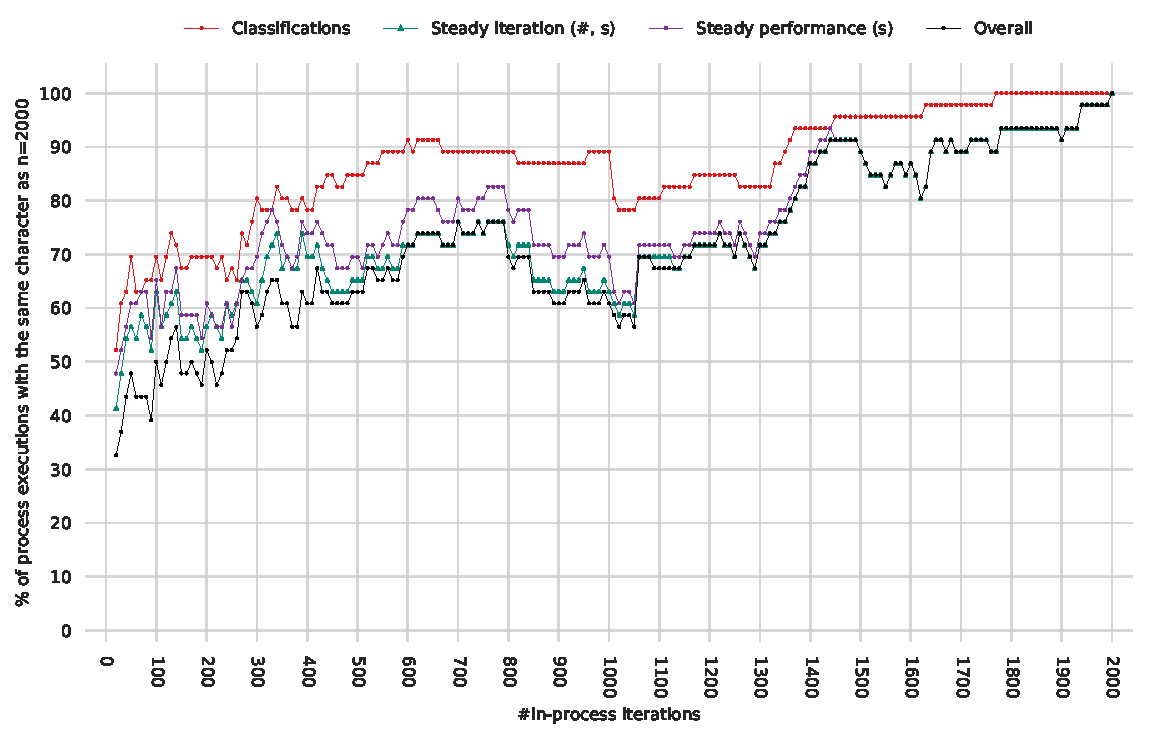
\includegraphics[width=\textwidth]{examples/truncated_same_plot.pdf}
\caption{How similar \bencherseven's data (seen in Figure~\ref{tab:mainresults}) data
would have been if we had run fewer than
\numiterations in-process iterations. We truncated process executions (taking in-process
iterations $0 \ldots n$ where $n \in \{10, 20, \ldots, 1980, 1990\}$) and compared
their classifications, time to reach a steady state, and steady state
performance to the original ($n=2000$). The `overall' similarity of each truncated
dataset is the number of \vmbpair pairs for which all three characteristics are statistically
equivalent to the full experiment.
In general, lower values of $n$ lead to fewer process executions
which are similar to $n=2000$. However, there is a very significant kink in the
data (with the trough between $1000 \leq n \leq 1300$), almost entirely caused by JRuby+Truffle (see
Figure~\ref{fig:truncated}).}
\label{fig:sametruncated}
\end{figure}

\begin{figure}[!tbp]
\centering
\begin{minipage}[t]{0.485\textwidth}
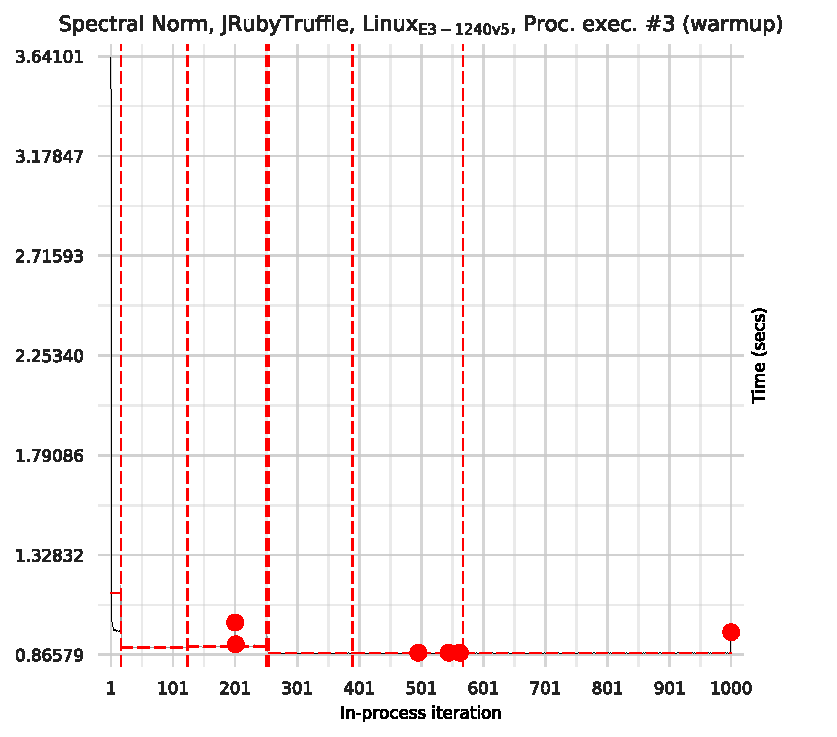
\includegraphics[width=\textwidth]{examples/truncated1.pdf}
\end{minipage}
\hfill
\begin{minipage}[t]{0.485\textwidth}
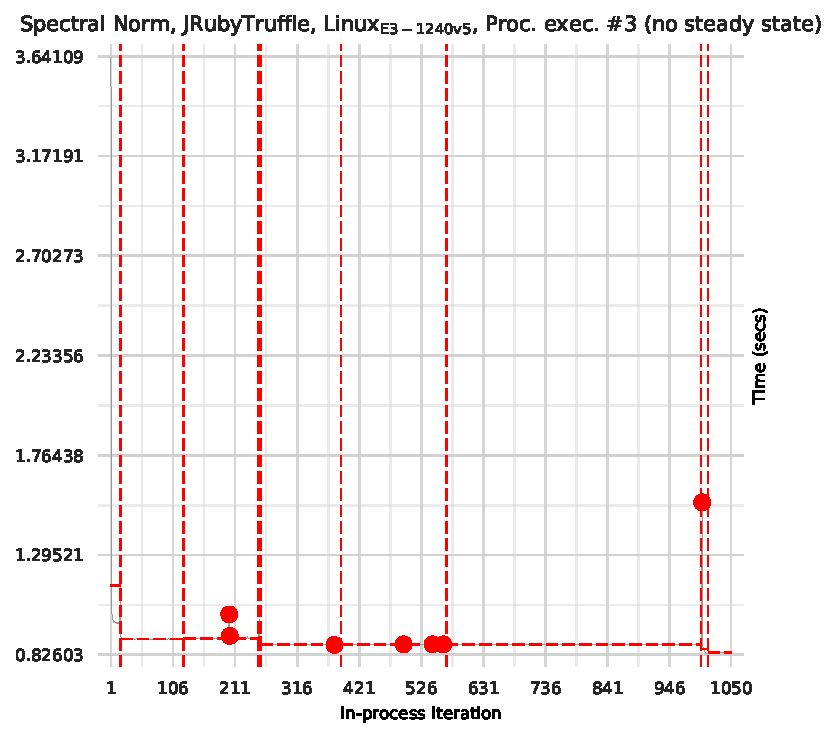
\includegraphics[width=\textwidth]{examples/truncated2.pdf}
\end{minipage}
\caption{Comparing the changepoints and classifications of a
single JRuby+Truffle process execution originally classified as warmup when
truncated at $n = 1000$ (LHS) and $n = 1050$ (RHS). Many JRuby+Truffle process
executions have a performance spike in between in-process iterations 1000 and
1050. Since the performance spike is entirely truncated at $n=1000$,
the resulting classification is the same as at $n=2000$. At $n=1050$,
enough of the performance spike \edd{it's not really a spike, is it? I'd expect
true spikes to be ignored as outliers. How about step? Rembember to update main
body too} is present to result in a new changepoint
segment,
that then causes a classification of no steady state.}
\label{fig:truncated}
\end{figure}

We chose \numiterations in-process iterations based on our experience of VMs' internals.
VMs have many counters which, when they exceed a certain threshold, cause the VM
to change behaviour (e.g.~(re)compile code, change garbage collection strategy
etc.). Our experience is that these counters are often set at `common for human'
values. Although many are likely to be set to small values, we knew that some
counters would be set to around 1000 (e.g.~tracing in RPython VMs such
as PyPy occurs at 1039 iterations of a loop) and that we might observe VM effects at in-process iterations
around this point. With that in mind, it was then necessary to
run benchmarks significantly past 1000 in-process iterations so that we would
be able to observe any long-term effects.

To understand whether we could have achieved similar quality results with fewer in-process
iterations, we truncated all of \bencherseven's process executions (for each process execution, taking
in-process iterations from $0 \ldots n$ where $n \in \{10, 20, \ldots, 1980, 1990\}$),
repeated the changepoint analysis, and compared the resulting
classifications, times to reach a steady state, and steady state performances to
the original ($n=2000$). We shrank the sliding window and last segment sizes
proportionally (i.e.~at $n=1000$ the sliding window is 100 and last segment
250).

Intuitively, one would expect the similarity to decrease as $n$ reduces, allowing
one to pick a value of $n$ that has a good trade-off between accuracy and running time.
As Figure \ref{fig:sametruncated} shows, there can be significant
kinks in the data that make choosing such a value tricky. In this case, the most
notable kink is between $1000 \leq n \leq 1300$. This is almost entirely caused by
JRuby+Truffle, many of whose \edd{reword ``many of whose''?} process executions have a distinct performance spike
just after in-process iteration 1000, often leading to a changepoint
segment being identified. At $n=2000$, changepoint analysis considers this slower
segment to be equivalent to the final segment (generally leading to a classification
of slowdown or warmup). At $n=1000$ the segment is not detected at all, generally
leading to a similar classification as at $n=2000$. At $n=1050$, however, a
segment is detected. Since it is the process execution's final segment,
and since it typically has a smaller mean and variance than the `real' last
segment, it is often considered non-equivalent to the preceding segment,
which then often leads to a classification of no steady state.
Figure \ref{fig:truncated} shows an example of this phenomenon.

\sarah{Will check these numbers again...}
It is thus difficult to draw definitive conclusions from our data:
at $n=650$ only 11\% of classifications would have changed,
but 21\% would have changed at $n=1050$.
It is clear that the quality of classifications
is heavily dependent on the VM(s) in question: if one is confident that the VM(s) in question do not have
semi-predictable performance spikes then it may be possible to run many fewer
in-process iterations; if one is unsure then running more is the only safe
course of action. We suggest that in many cases a reasonable compromise might be to
use smaller numbers (e.g.~500) of in-process iterations most
of the time, while occasionally using larger numbers (e.g.~1500) to see if
longer-term stability has been affected.


\subsubsection{Process executions}

\begin{figure}[tbp]
\centering
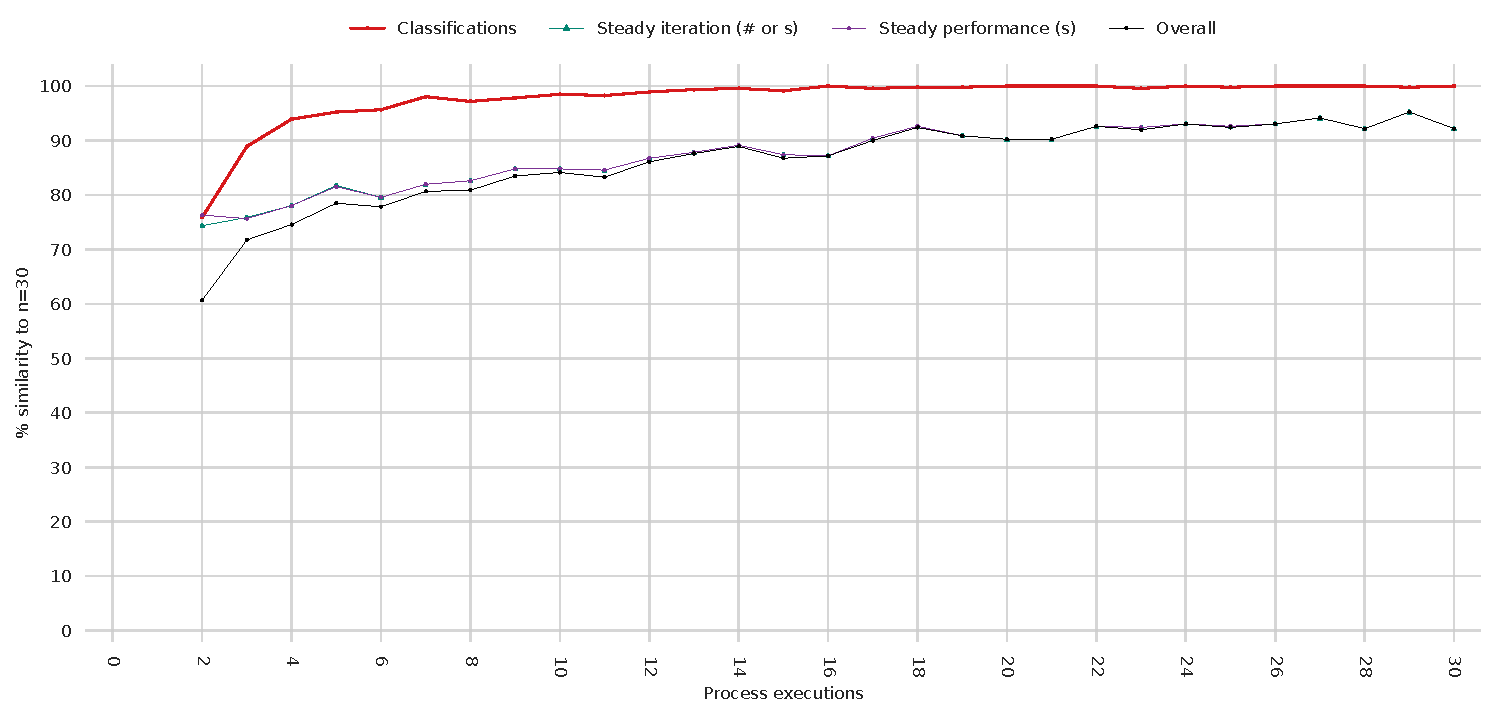
\includegraphics[width=\textwidth]{examples/truncated_pexecs_plot.pdf}
\caption{How similar \bencherseven's data (seen in Figure~\ref{tab:mainresults}) data
would have been if we had run fewer than
\numpexecs process executions. From the original \bencherseven dataset, we created \laurie{$1000$} samples
of $n$ process executions with replacement (where $n \in {2, 3, \ldots, 29,
30}$) and compared their classifications, time to reach a steady state, and
steady state performance to the original ($n=30$). The `overall' similarity of
each truncated dataset is the number of \vmbpair pairs for which all three
characteristics are statistically equivalent to the full experiment. In general,
lower values of $n$ lead to fewer process executions which are similar to
$n=30$.} \label{fig:pexecstruncated}
\end{figure}

\sarah{Check 1000 trials before submission.}
We had little intuition as to how many process executions we should run, so our
eventual choice of \numpexecs was somewhat arbitrary. To understand if we could
have used fewer process executions, we used a slightly different method
to the analysis of in-process iterations. We took the \bencherseven data set and
for each $n \in \{2, 3, \ldots, 29, 30\}$ we bootstrapped \laurie{1000? 10000?}
samples (using sampling with replacement) of size $n$. To enable us to compare
inconsistent classifications between sets, we constructed multinomial proportion confidence
intervals (i.e.~the proportion of warmup, slowdown, flat and no
steady state classifications) on the original set and each sampled set using the
method of \cite{sison95simultaneous}. One unintuitive side effect of sampling is that
the $n = 30$ sample does not lead to 100\% similarity. Consider a \vmbpair
which has 29 warmup process executions and 1 no steady state process execution.
If a sample of 30 warmup process executions is created, then all three
comparisons (classification, steady iter (\#), and steady perf (s)) will fail,
reducing each similarity rating below 100\%. Bearing that in mind, Figure
\ref{fig:pexecstruncated} shows the results of this analysis.

\laurie{needs redoing}
Our analysis suggests that 15 process executions is a reasonable, and realistic, figure for most
cases, yielding similar quality data to the 30 that we ran. As with in-process
iterations, occasionally running larger numbers of process executions will help
identify infrequent performance issues.


\section{Conclusions}
\label{sec:conclusions}

Warmup has previously been an informally defined term~\cite{seaton15phd}. We
captured a restricted version of this definition in Hypothesis H1, which
a carefully designed experiment then invalidated. The analysis
techniques we used are open-source and can be used by VM developers and users to investigate the
warmup behaviour of any VM and benchmark.

Although we are fairly experienced in designing and implementing
experiments, the experiment in this paper took far more time than we expected
--- around 3 person years. In part this is because there is limited precedent for such detailed
experiments. Investigating possible confounding variables, understanding how to
control them, and implementing the necessary checks, all took time. In many
cases, we had to implement small programs or systems to understand a variable's
effect (e.g.~that Linux allows a process to allocate memory beyond that
specified in the soft and hard \texttt{ulimit}). However, we are realistic that
few people will have the time or energy to institute all the controls that we
implemented. An open question is which of the controls are the most significant
in terms of producing a reliable experiment. The large number of partly
inter-locking combinations means that we estimate that untangling this will
require significant additional running time (at least many months).


\begin{acks}
We are particularly grateful to Vincent Knight who helped put together this
paper's team. Chris Seaton helped integrate JRuby+Truffle into our experiment.
Lukas Diekmann rebooted more servers than any person should have to.
We also thank (in alphabetical order) Dave Dice, Kenny Gross, Tim Harris, Tomas Kalibera, Ben
Titzer, Mircea Trofin, Dave Ungar, and Mario Wolczko for comments and suggestions; any
errors and infelicities are our own. This research was funded by the EPSRC
Cooler (EP/K01790X/1) grant and Lecture (EP/L02344X/1) fellowship,
and a gift from Oracle Labs.

\textbf{Transparency:} Three of this paper's authors have contributed
to the PyPy project, and one is an OpenBSD developer. The
King's group has received several funding gifts from Oracle Labs.
\end{acks}


\bibliography{bib}

\clearpage

\appendix

\noindent In this appendix, we first show that our statistical method
can be applied to well known benchmarking suites (Appendix~\ref{sec:existing})
before showing additional results from the main part of our experiment
(Appendix~\ref{app:mainresults}). We
then present a curated selection of interesting run-sequence
plots (Appendix~\ref{sec:curatedplots}). The complete series of plots is available in a separate
document.


\section{Applying the Statistical Method to Existing Benchmark Suites}
\label{sec:existing}

The statistical method presented in Section~\ref{sec:stats} is not limited to data
produced from Krun. To demonstrate this, we have applied it to two standard
benchmark suites: the DaCapo suite for Java~\cite{dacapo06} and the Octane
suite for JavaScript~\cite{octane}. Octane was
run on all three of our benchmarking machines, whereas (due to time
constraints), Dacapo was run only on \bencherfive. For both suites we used
\numpexecs process executions and \numiterations in-process iterations.

We ran DaCapo (with its default benchmark size) on Graal and HotSpot. As it already has support for
altering the number of in-process iterations, we used it without modification.
However, we were unable to run 3 of its 14 benchmarks: \texttt{batik}
crashes with a \texttt{Invocation\-Target\-Exception}; \texttt{eclipse},
\texttt{tomcat} fail their own internal validation checks. We experienced
semi-regular hangs with Graal which led us to disable \texttt{luindex},
\texttt{tradebeans}, and \texttt{tradesoap} on Graal only.

We ran Octane on the same version of V8 used in the main experiment, and (on
Linux only, due to benchmark failures on OpenBSD) on SpiderMonkey
(\spidermonkeyversion, a JIT compiling VM for JavaScript).
We replaced its complex runner (which reported timings with a non-monotonic
microsecond timer) with a simpler alternative (using a monotonic millisecond
timer). We also had to decide on an acceptable notion of `iteration'. Many of Octane's
benchmarks consist of a relatively quick `inner benchmark'; an `outer benchmark'
specifies how many times the inner benchmark should be run in order to make an
adequately long in-process iteration\edd{note that our krun benchmarks are the
same. Is it even worth mentioning?} . We recorded \numiterations
in-process iterations of the outer benchmark; our runner
fully resets the benchmark and the random number generator between each
iteration. The \texttt{box2d}, \texttt{gameboy}, \texttt{mandreel} benchmarks do
not properly reset their state between runs, leading to run-time errors we have
not been able to fix; \texttt{typescript}'s reset function, in contrast,
frees constant data needed by all iterations, which we were able
to easily fix. When run for \numiterations iterations, \texttt{CodeLoadClosure},
\texttt{pdfjs}, and \texttt{zlib} all fail due to memory leaks. We were able to
easily fix \texttt{pdfjs} by emptying a global list after each iteration, but not the
others. We therefore include 12 of Octane's benchmarks (including lightly
modified versions of \texttt{pdfjs} and \texttt{typescript}).
Because we run fewer benchmarks, our modified runner is unable to fully
replicate the running order of Octane's original runner. Since Octane runs all
benchmarks in a single process execution, this could affect the performance of
later benchmarks in the suite.

Table~\ref{tab:dacapo} shows the full DaCapo results. Because we had to run
a subset of benchmarks on Graal, a comparison with HotSpot is difficult
though of the benchmarks both could run, there is a reasonable degree
of similarity. However, even on this most carefully designed of benchmark suites, only 42\%
of \vmbpair pairs have `good' warmup.

Tables~\ref{tab:octaneb5}--\ref{tab:octaneb7} show the full Octane results. These
show a greater spread of classifications than the DaCapo results, with
33\% of \vmbpair pairs over the three machines having `good' warmup.

As these results show, our automated statistical method produces satisfying
results even on existing benchmark suites that have not been subject to the
\krun treatment. Both DaCapo and (mostly) Octane use much larger benchmarks than
our main experiment. We have no realistic way of understanding to what extent
this makes `good' warmup more or less likely. For example, it is likely that
there is CFG non-determinism in many of these benchmarks; however, their larger
code-bases may give VMs the ability to `spread out' VM costs, making smaller
blips less noticeable.

\begin{landscape}
\begin{table*}[htp]
\caption{DaCapo results for \bencherfive.}
\centering
\begin{adjustbox}{scale=.9}
\input{dacapo.table}
\end{adjustbox}
\label{tab:dacapo}
\end{table*}
\end{landscape}


\begin{landscape}
\begin{table*}[htp]
\caption{Octane results for \bencherfive.}
\centering
\begin{adjustbox}{scale=.9}
\input{bencher5_octane.table}
\end{adjustbox}
\label{tab:octaneb5}
\end{table*}
\end{landscape}

\begin{table*}[htp]
\centering
\caption{Octane results for \benchersix.}
\begin{adjustbox}{scale=.9}
\input{bencher6_octane.table}
\end{adjustbox}
\label{tab:octaneb6}
\end{table*}

\begin{landscape}
\begin{table*}[htp]
\caption{Octane results for \bencherseven.}
\centering
\begin{adjustbox}{scale=.9}
\input{bencher7_octane.table}
\end{adjustbox}
\label{tab:octaneb7}
\end{table*}
\end{landscape}

\section{Further Results}
\label{app:mainresults}
\label{app:dacapo}
\label{app:octane}

\noindent The main experiment's results for \bencherfive and \benchersix can be
seen in Tables~\ref{tab:bencher5results} and \ref{tab:bencher6results}.

\begin{landscape}
\begin{table*}[t]
\caption{Benchmark results for \bencherfive.}
\centering
\begin{adjustbox}{scale=.85} % This table is BIG.
\input{bencher5.table}
\end{adjustbox}
\label{tab:bencher5results}
\end{table*}
\end{landscape}

\begin{landscape}
\begin{table*}[t]
\captionof{table}{Benchmark results for \benchersix.}
\centering
\begin{adjustbox}{scale=.9}
\input{bencher6.table}
\end{adjustbox}
\label{tab:bencher6results}
\end{table*}
\end{landscape}


\clearpage
\onecolumn

\section{Curated Plots}
\label{sec:curatedplots}

\noindent The remainder of this appendix shows curated plots: we have selected
4 interesting plots from each classification, to give readers a sense of
the range of data obtained from our experiment. A separate document contains the
complete series of plots.

\clearpage

\subsection{Examples of Warmup Behaviour}

\vfill%
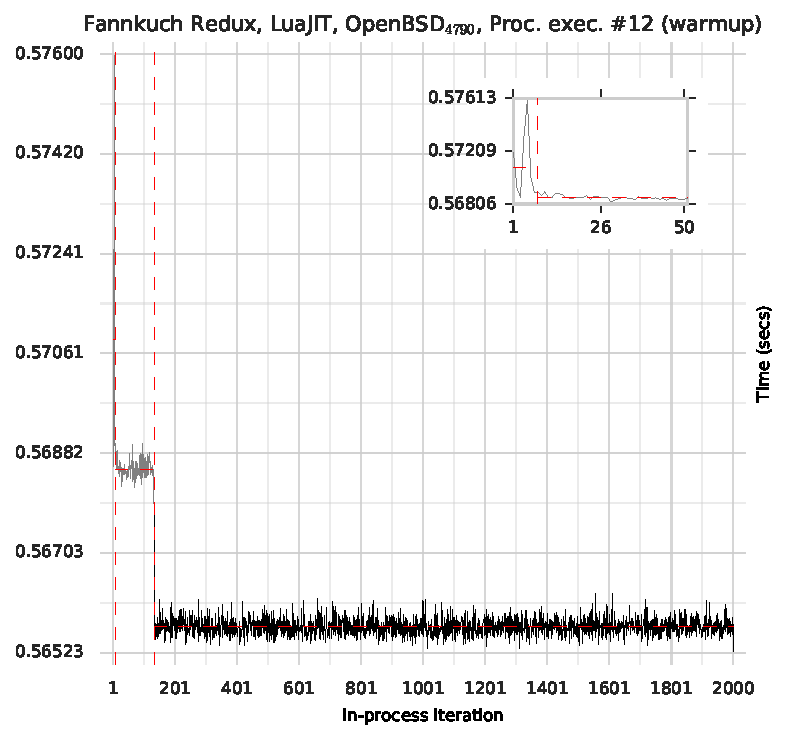
\includegraphics[width=.49\textwidth]{category_examples/warmup/warmup0.pdf}%
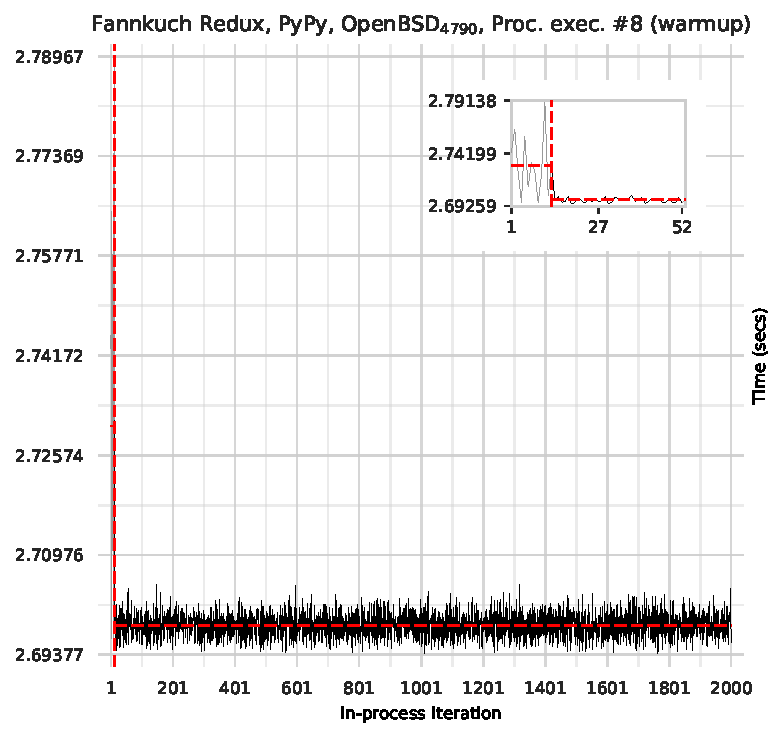
\includegraphics[width=.49\textwidth]{category_examples/warmup/warmup1.pdf}%
\vfill%
\noindent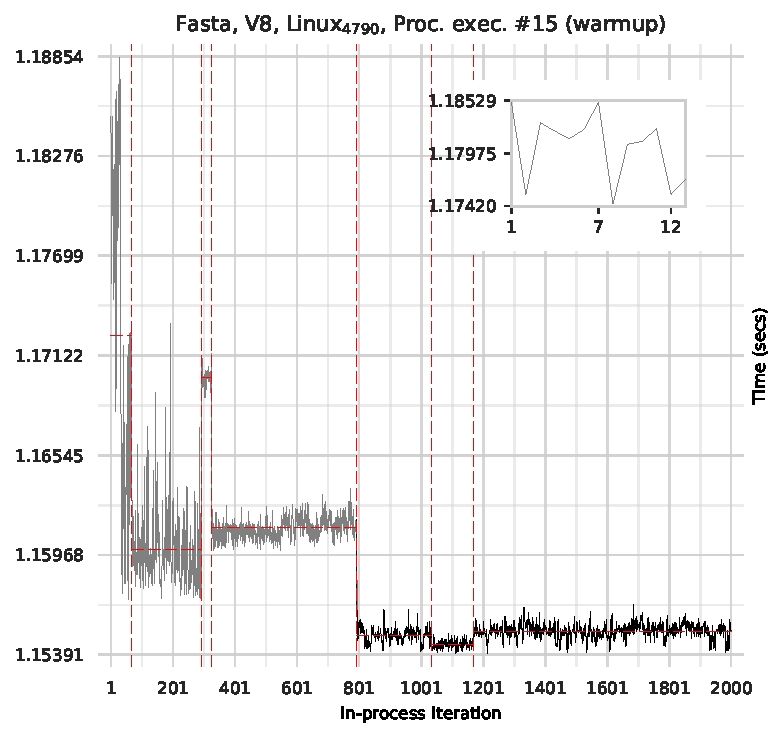
\includegraphics[width=.49\textwidth]{category_examples/warmup/warmup2.pdf}%
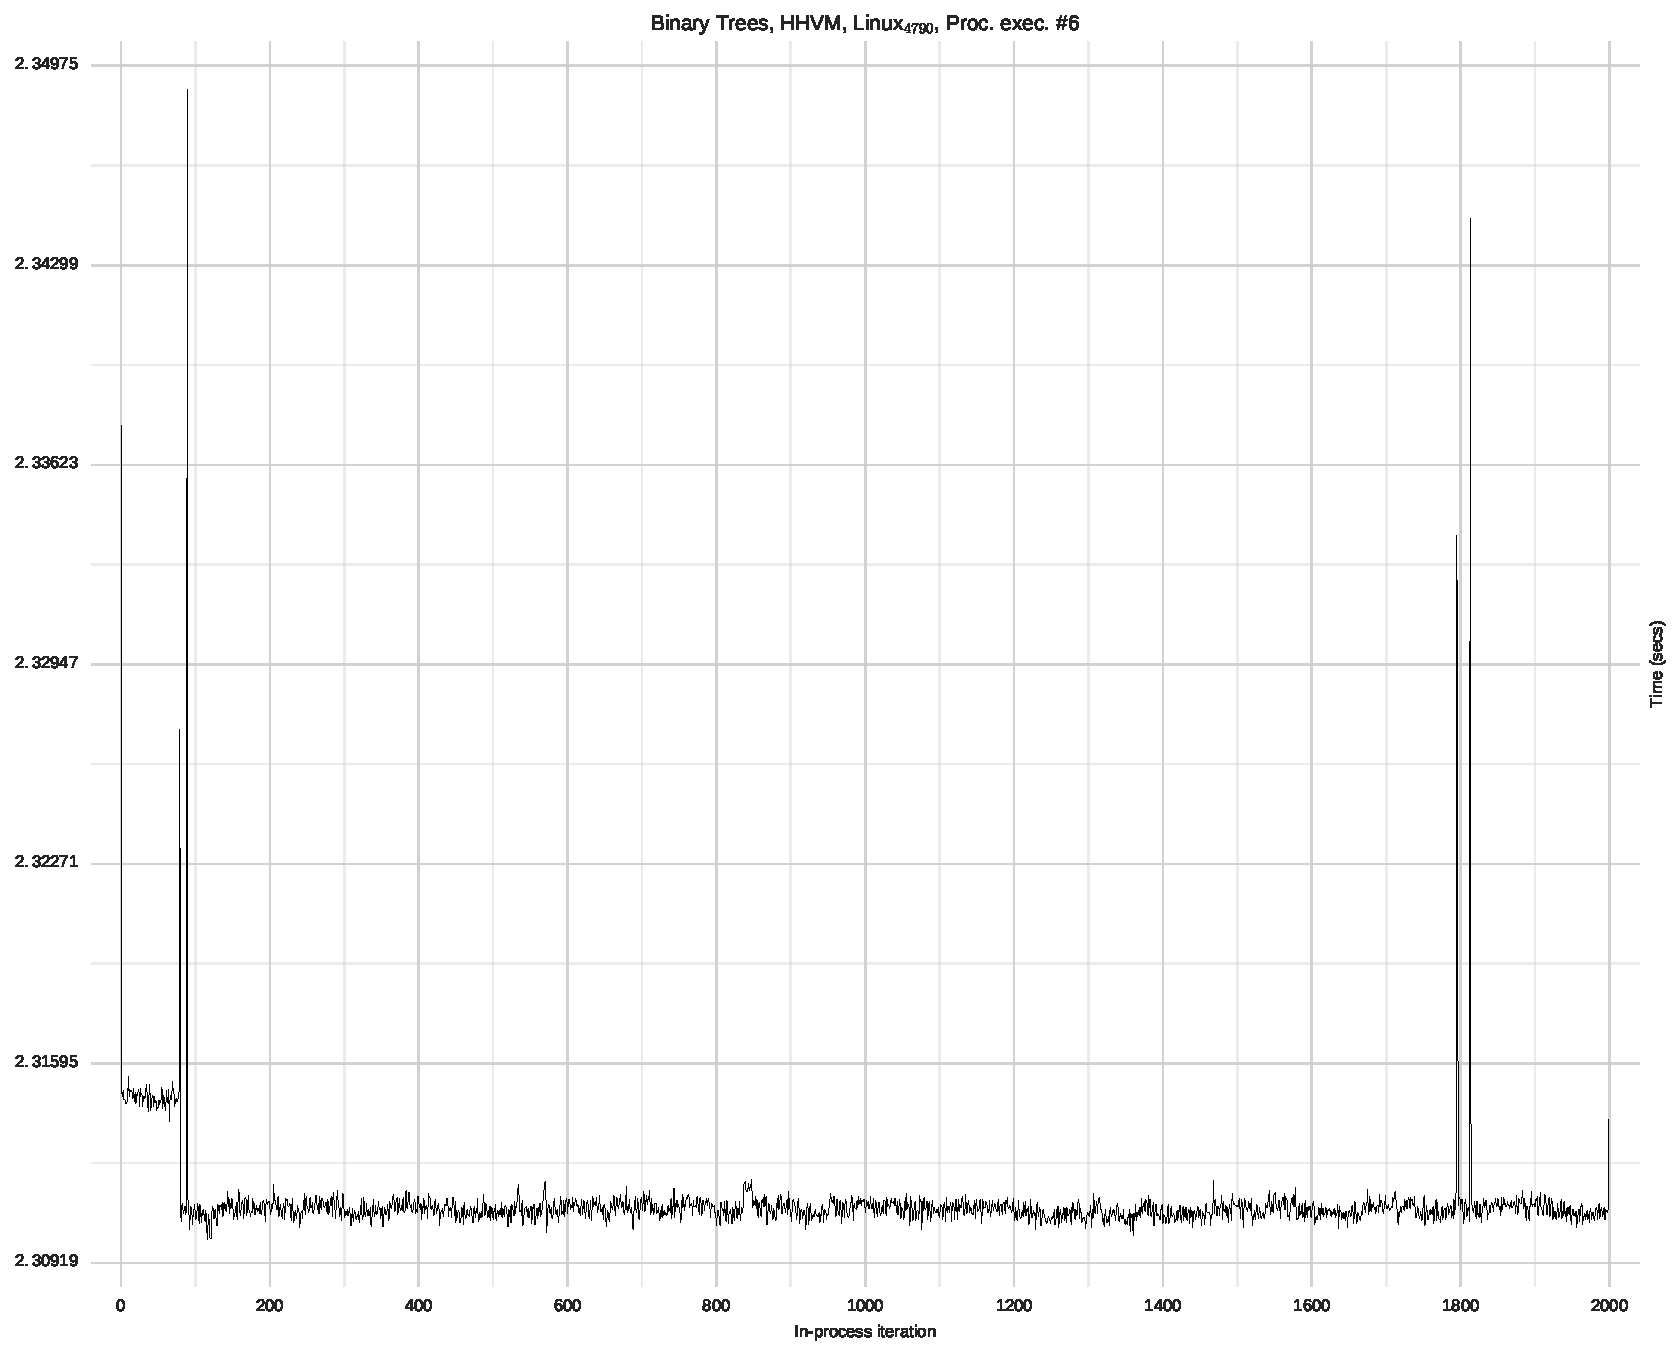
\includegraphics[width=.49\textwidth]{category_examples/warmup/warmup3.pdf}%
\vfill%

\clearpage
\subsection{Examples of Flat Behaviour}

\vfill%
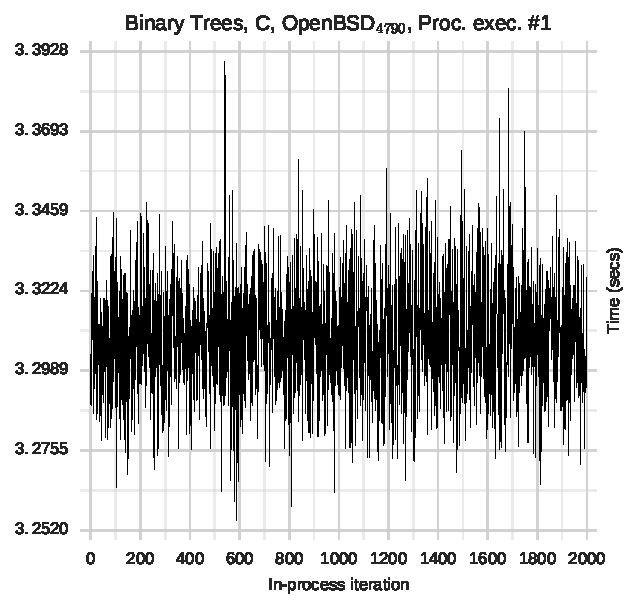
\includegraphics[width=.49\textwidth]{category_examples/flat/flat0.pdf}%
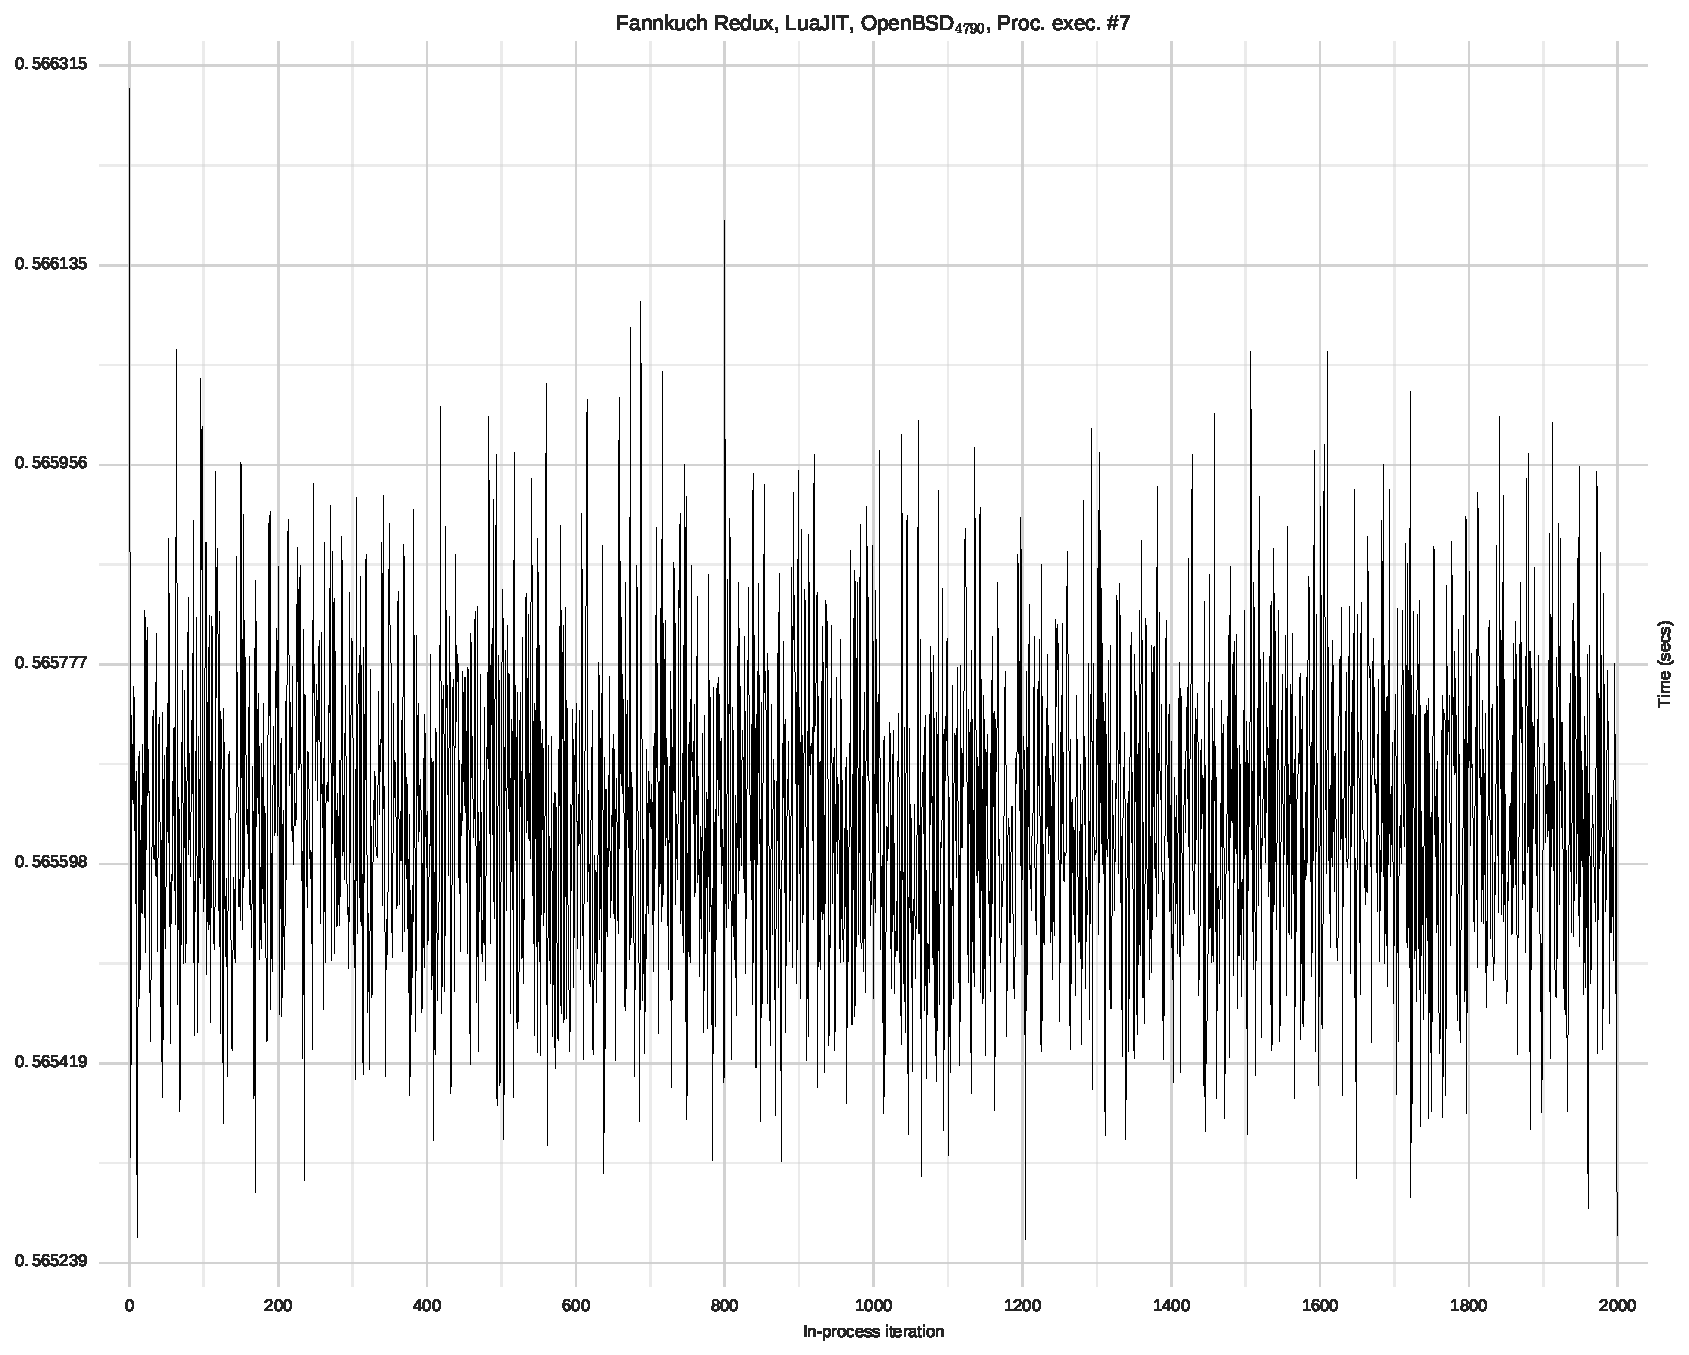
\includegraphics[width=.49\textwidth]{category_examples/flat/flat1.pdf}%
\vfill%
\noindent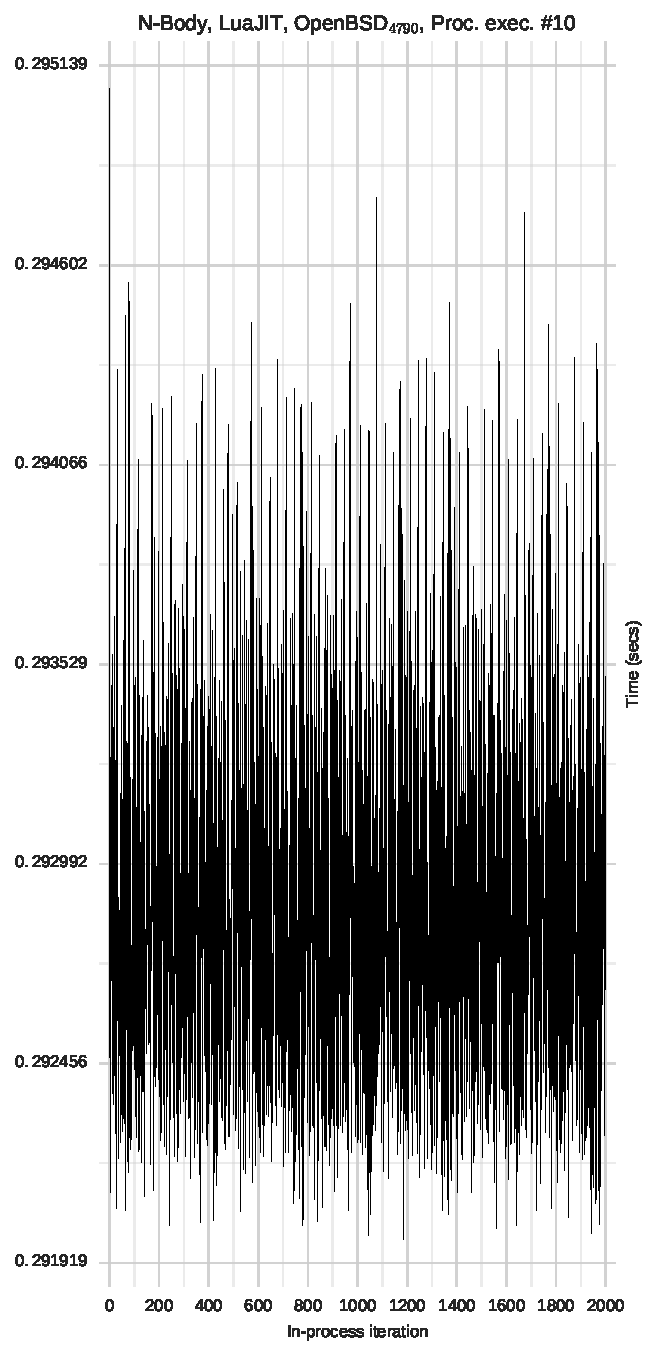
\includegraphics[width=.49\textwidth]{category_examples/flat/flat2.pdf}%
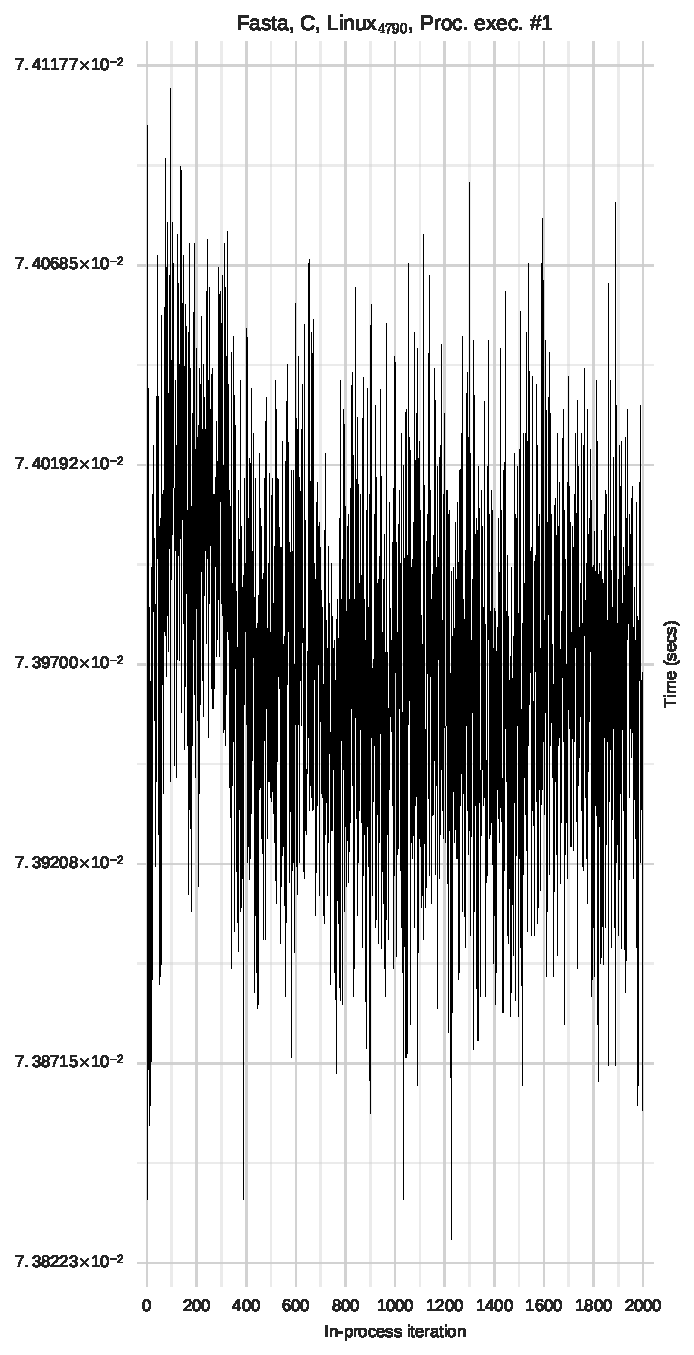
\includegraphics[width=.49\textwidth]{category_examples/flat/flat3.pdf}%
\vfill%

\clearpage
\subsection{Examples of Slowdown Behaviour}
\vfill%
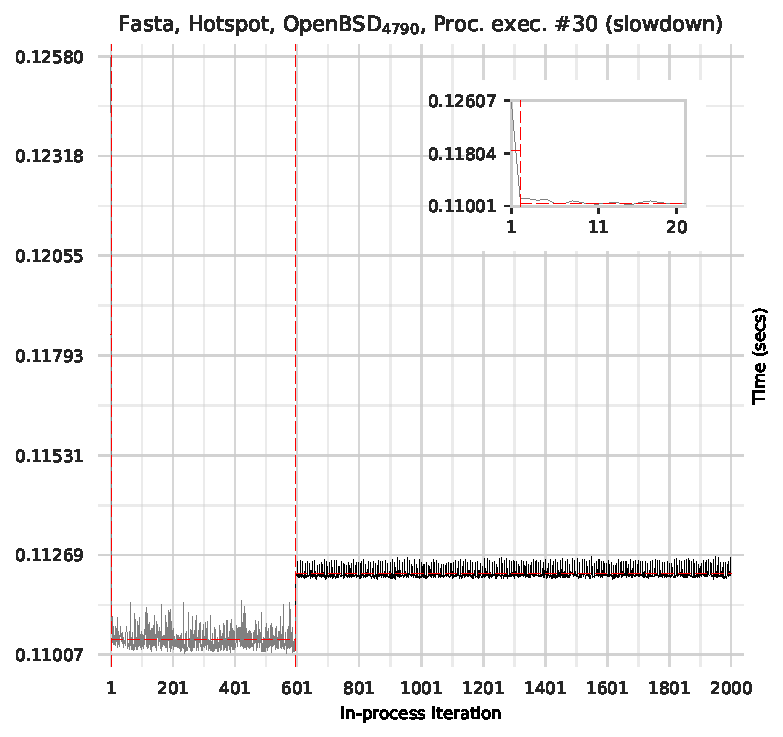
\includegraphics[width=.49\textwidth]{category_examples/slowdown/slowdown0.pdf}%
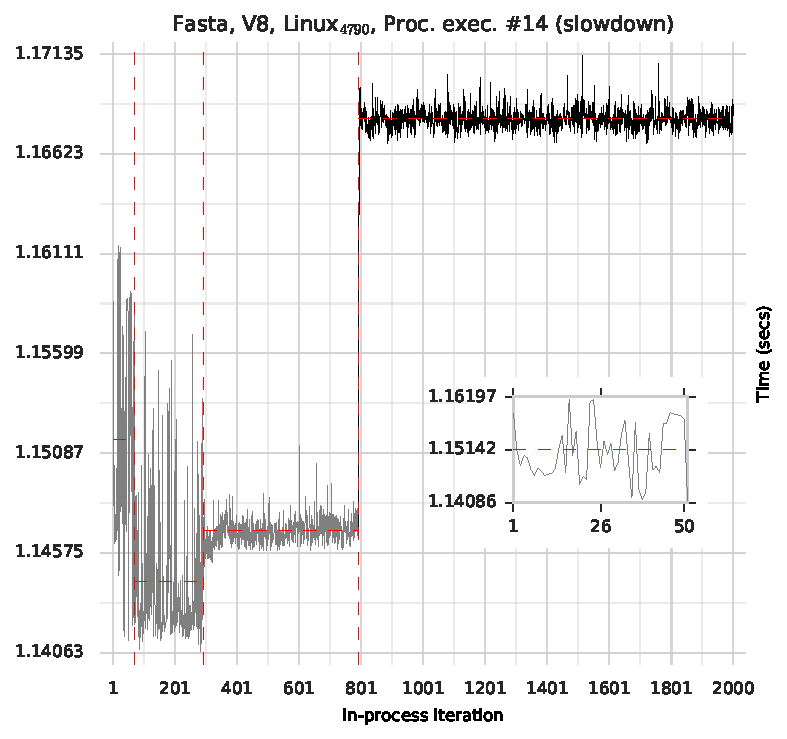
\includegraphics[width=.49\textwidth]{category_examples/slowdown/slowdown1.pdf}%
\vfill%
\noindent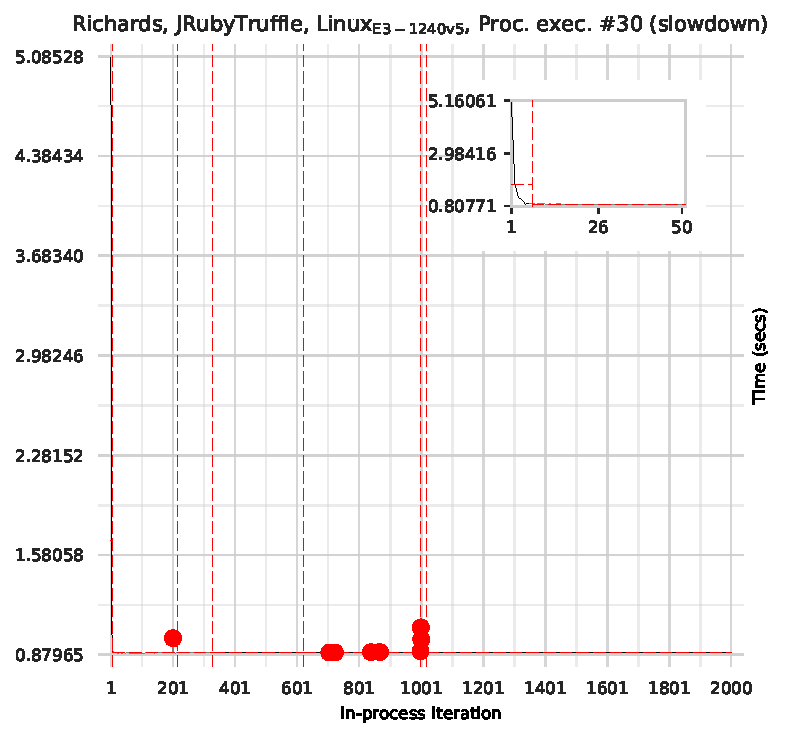
\includegraphics[width=.49\textwidth]{category_examples/slowdown/slowdown2.pdf}%
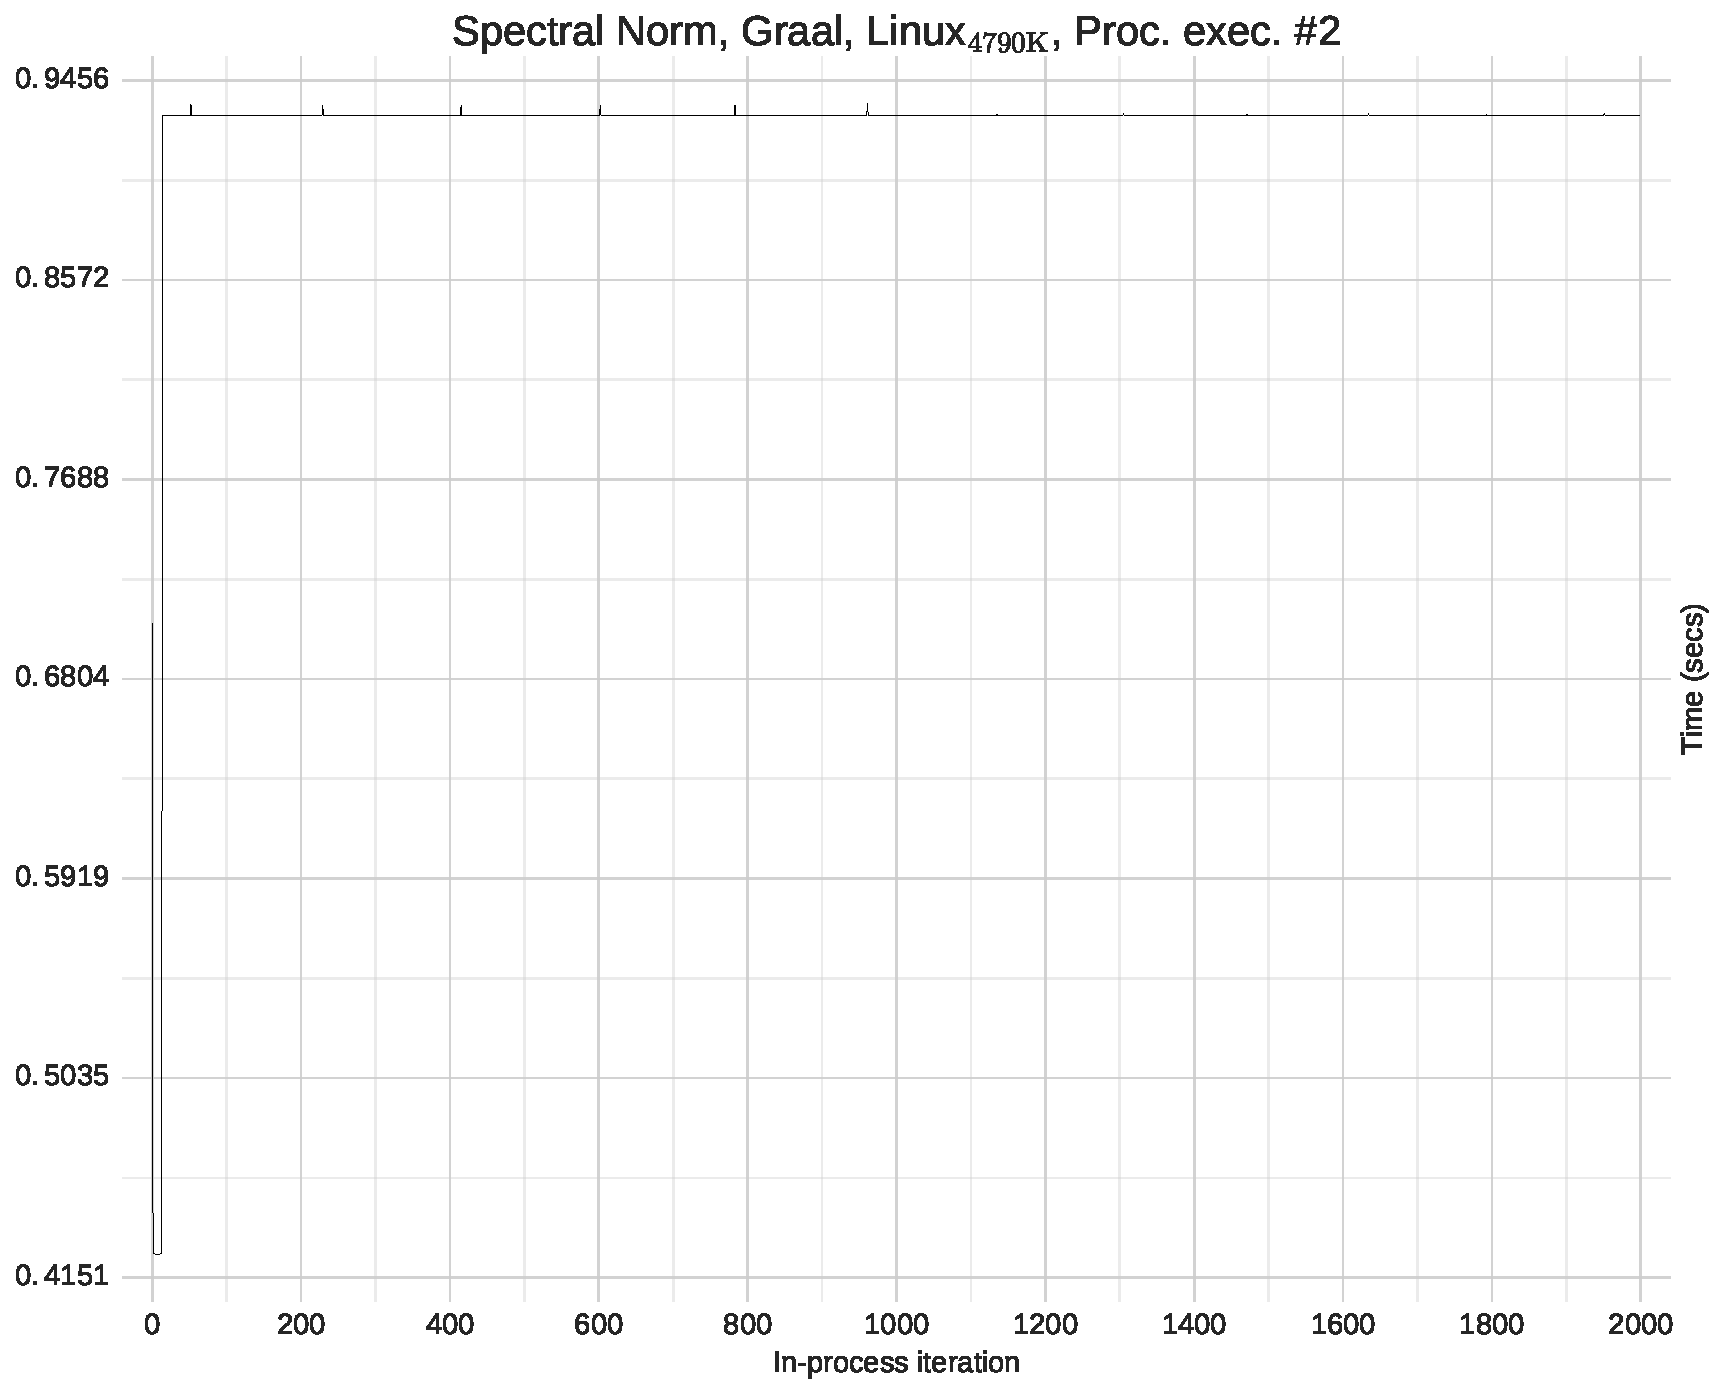
\includegraphics[width=.49\textwidth]{category_examples/slowdown/slowdown3.pdf}%
\vfill%

\clearpage
\subsection{Examples of No Steady State Behaviour}

\vfill%
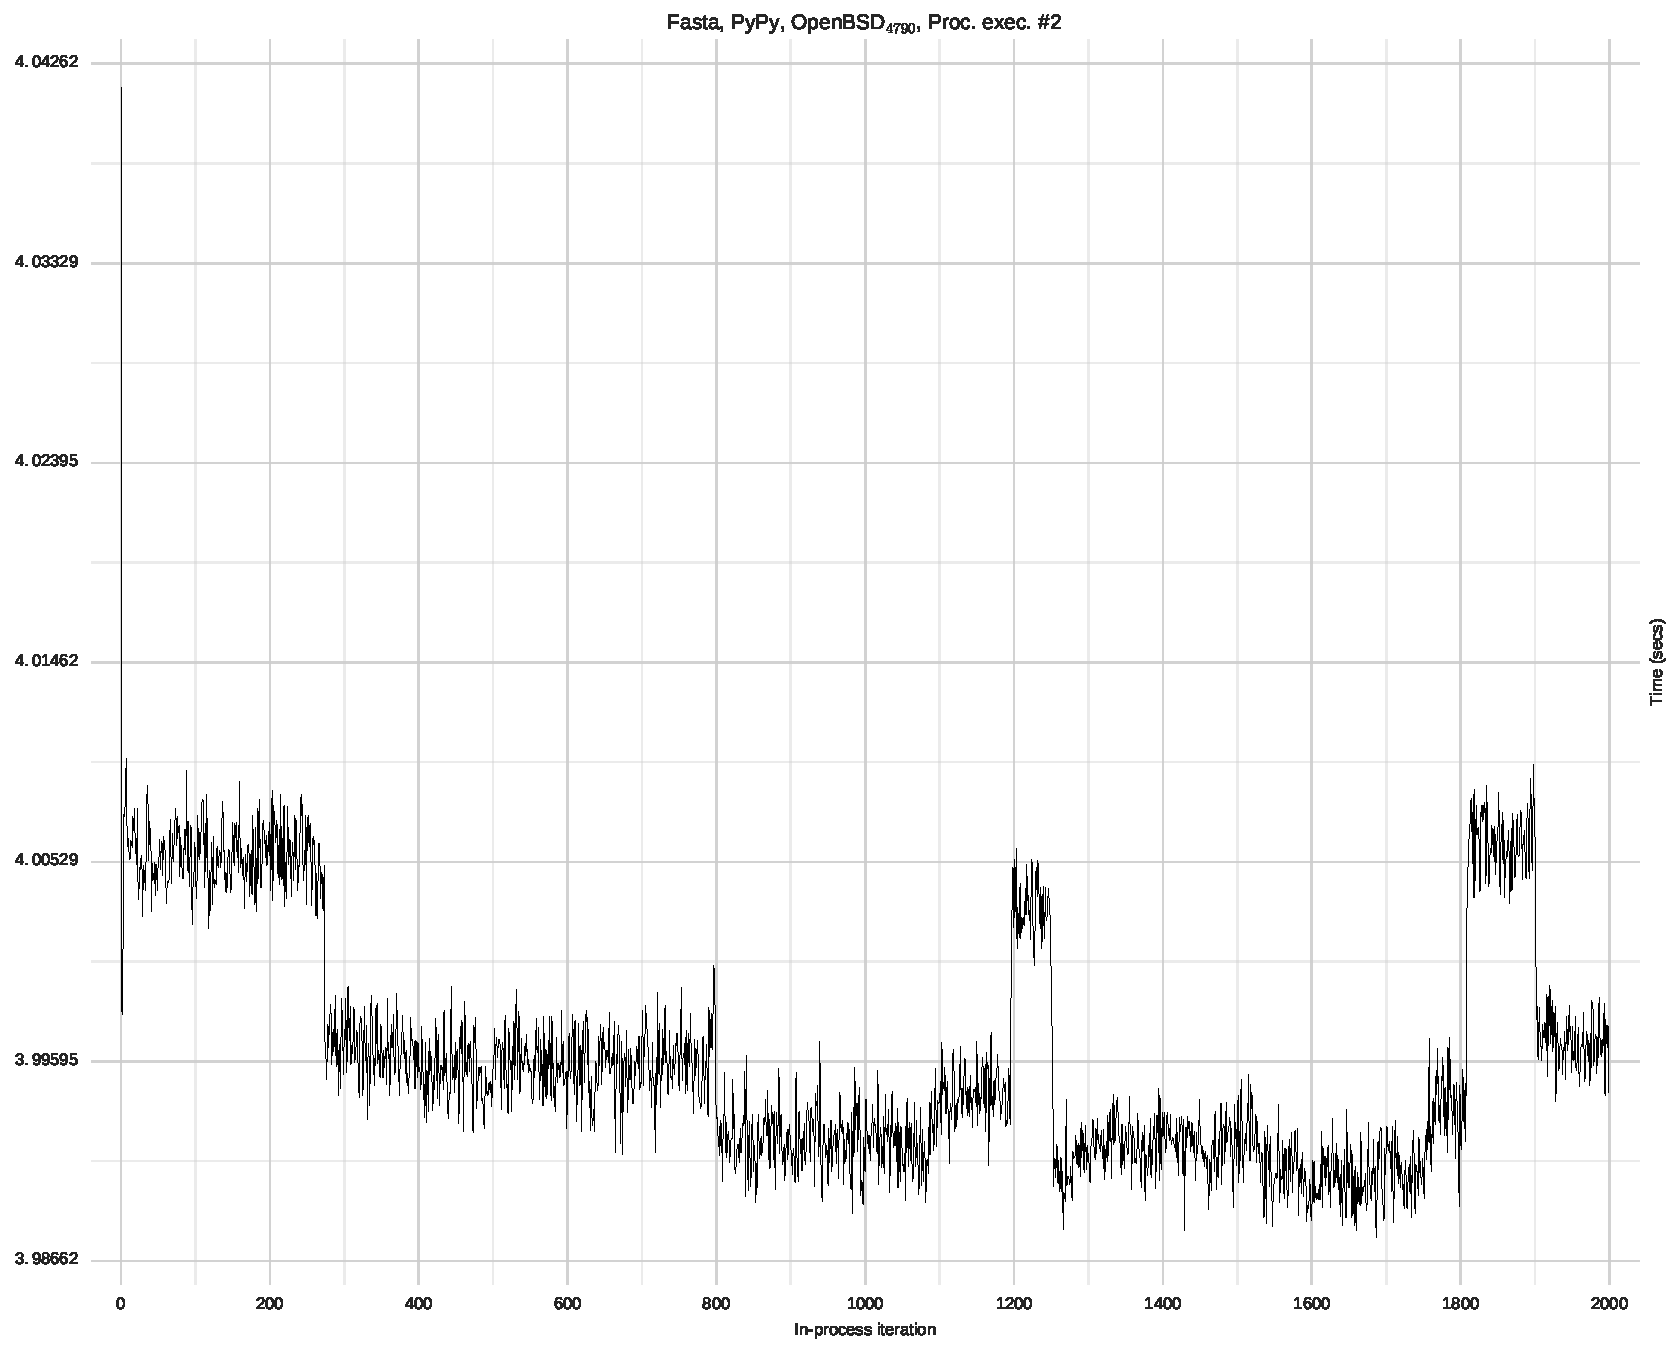
\includegraphics[width=.49\textwidth]{category_examples/nosteadystate/nosteadystate0.pdf}%
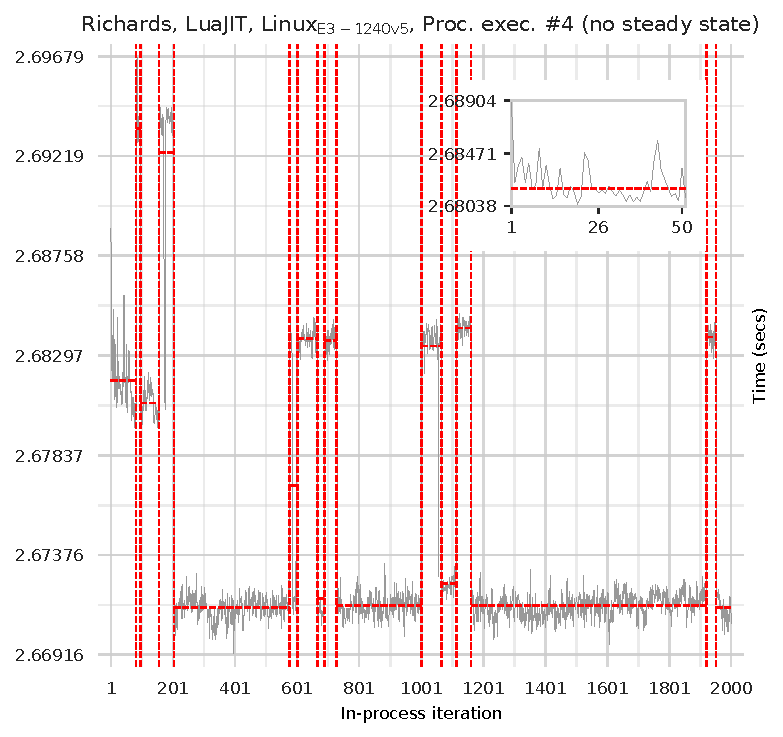
\includegraphics[width=.49\textwidth]{category_examples/nosteadystate/nosteadystate1.pdf}%
\vfill%
\noindent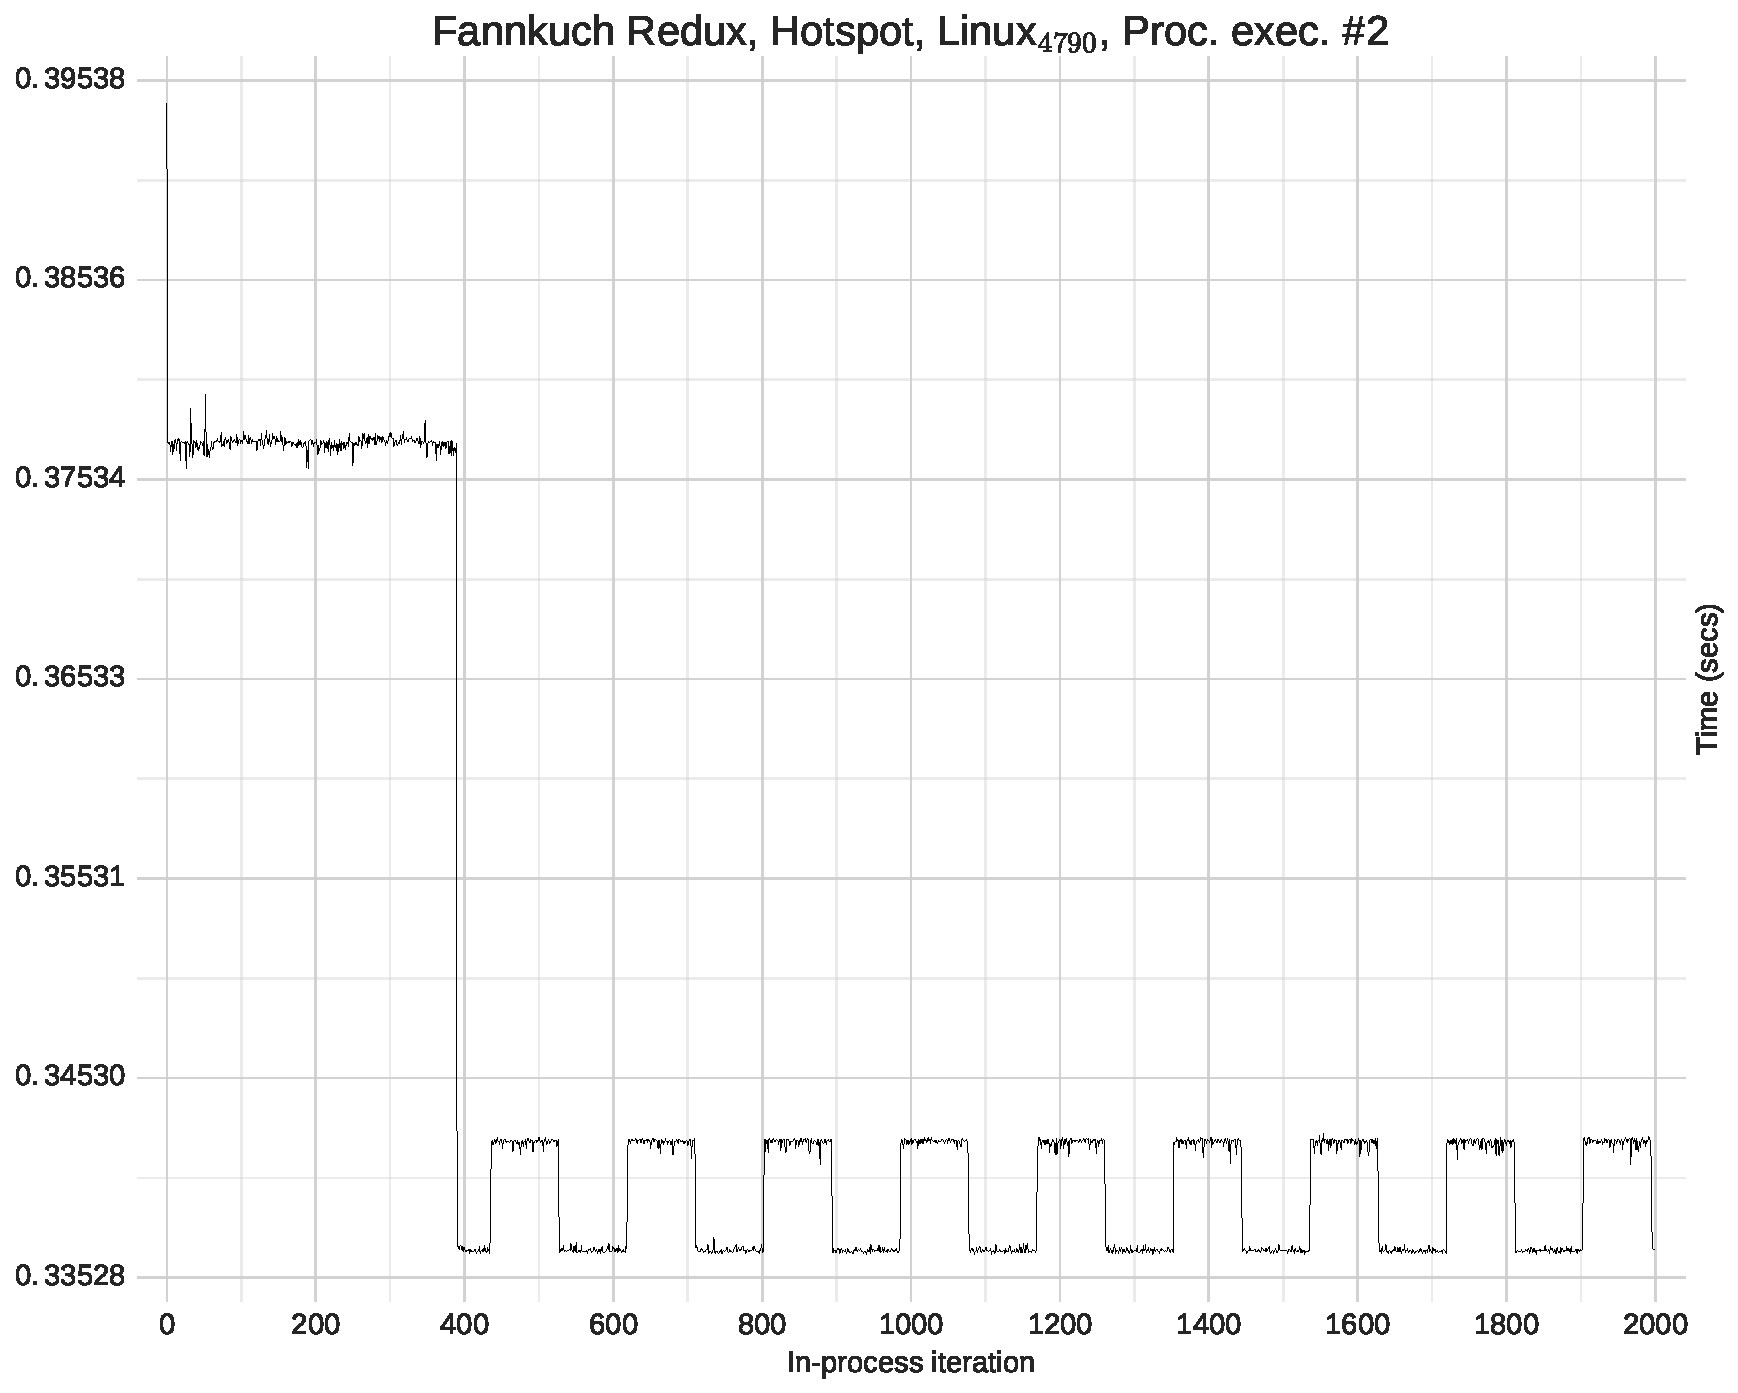
\includegraphics[width=.49\textwidth]{category_examples/nosteadystate/nosteadystate2.pdf}%
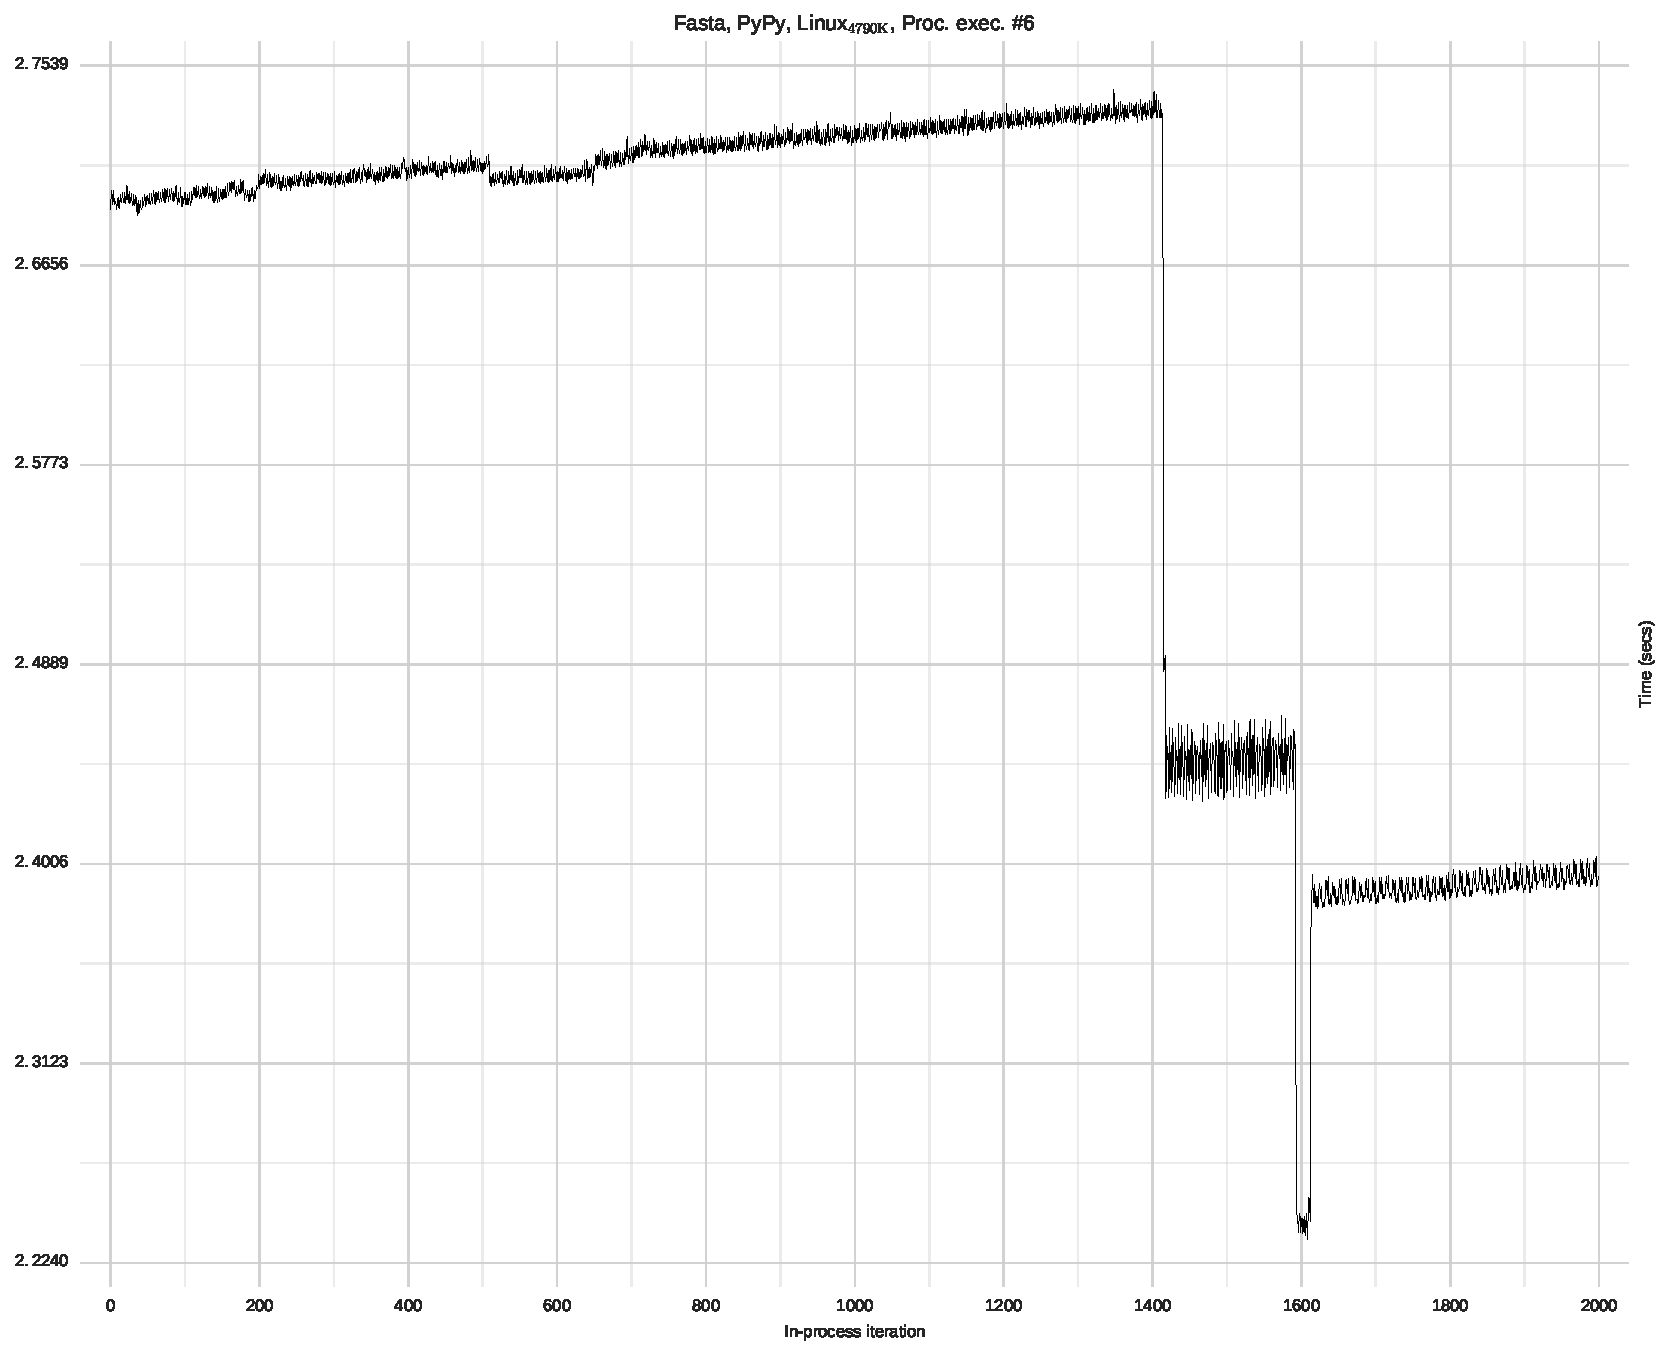
\includegraphics[width=.49\textwidth]{category_examples/nosteadystate/nosteadystate3.pdf}%
\vfill%

\end{document}
